\documentclass[review]{siamart0516}
%%\usepackage{lgrind}

%\usepackage[square,comma,numbers,sort&compress]{natbib}
%\usepackage{amsmath,amsthm,amssymb,amsfonts,amsbsy,latexsym} %amsthm inclusion conflicts with sisc...
\usepackage{amsmath,amssymb,amsfonts,amsbsy,latexsym}
\usepackage{graphics}
%\usepackage{epsfig}
%%\usepackage[hang,raggedright]{subfigure}
%\usepackage{epsf}
%\usepackage{setspace}
%\usepackage{hangcaption}
\usepackage{graphicx}    % needed for including graphics e.g. EPS, PS
\usepackage{multirow}
%\usepackage{threeparttable}
\usepackage{cancel}
\usepackage{enumerate}
\usepackage{color}
\usepackage{hyperref}

%\usepackage{algorithmicx}
%\usepackage[ruled]{algorithm}
\usepackage{algpseudocode}
\usepackage{varwidth}
%\usepackage{caption}
%\usepackage[font=small]{subcaption}
%\usepackage{longtable}
\usepackage{mathrsfs}
\usepackage{upgreek}
\usepackage[caption=false]{subfig} % for \subfloat

\hypersetup{
    colorlinks=true,       % false: boxed links; true: colored links
    linkcolor=black,          % color of internal links
    citecolor=black,        % color of links to bibliography
    filecolor=magenta,      % color of file links
    urlcolor=blue           % color of external links
}

\newcommand{\R}{{\mathbb{R}}}
\newcommand{\Reals}{{\mathbb{R}}}
\newcommand{\bit}{\begin{itemize}}
\newcommand{\eit}{\end{itemize}}
\newcommand{\red}[1]{{\color{red}{#1}}}
\newcommand{\orderof}[1]{{\ensuremath{ {\cal O}(#1)}}}

%\newtheorem{theorem}{Theorem} %conflicts with sisc

\graphicspath{{./figures/}}

\begin{document}
\raggedbottom %avoid weird vertical justification

\title{Model Adaptivity for Goal-Oriented Inference using Adjoints}

\author{Harriet Li, Vikram Garg, Karen Willcox}
%\date{}
\maketitle

\begin{abstract}
\red{Inference problems are often constrained by state equations, which arise from conservation laws, and constitutive relations. Often, a hierarchy of models can be derived from such laws and relations, reflecting varying fidelity versus cost tradeoffs. We introduce a goal-oriented, model adaptive, inference algorithm, which allows users to achieve an arbitrary error tolerance, while minimizing the use of high fidelity constraints. Numerical experiments exercise the algorithm on a highly nonlinear inverse problem, and showcase the computational savings and robustness benefits of this new approach.}

\end{abstract}

\begin{keywords}
  \red{keywords here}
\end{keywords}

\begin{AMS}
  \red{AMS codes here?}
\end{AMS}

\section{Introduction}

Parameter estimation/inference is an important component of mathematical modeling. The ability to infer parameters via an inverse problem allows practitioners to gain important information about systems, processes and the models that are used to describe them. Such inference also avoids intrusive experiments, which may otherwise be prohibitively expensive or impractical. Once parameters have been inferred via an inverse problem, they can be used for forward propagation of the model and, computing relevant quantities of interest for the modeling/decision making process.

Data, constraints and prior information form the critical components of an inverse problem formulation. There is an extensive literature pertaining to all these components, including the filtering of noise in data~\cite{}, the choice of regularization or representation of prior information~\cite{}, the efficient incorporation of constraints in solving the problem~\cite{}, and so on. Specifically, the work on the constraints defined by `state equations' in the inverse problem focuses on reducing the computational expense of solving the models that represent them. Such work includes the use of reduced order models to represent constraints~\cite{} and adaptive mesh refinement to control the size of the state equation discretizations~\cite{BecVex05,}, among other strategies.

Models that represent phenomena and processes can usually be organized in a hierarchy according to their fidelity and/or expense. The use of multiple models simultaneously for forward simulation is well established. Two main strategies exist for combining models: hierarchical and concurrent methods. Hierarchical methods (also known as information-passing or sequential methods) take the results of a simulation using the high-fidelity model and use them to inform a lower-fidelity model that is used globally (for example, modeling the molecular structure of a material to determine parameters for constitutive equations~\cite{Haoetal03}). In this work, we focus on multi-fidelity models formed using concurrent methods, which simultaneously solve the higher- and lower-fidelity models in different parts of the domain. For example, in~\cite{Khareetal08} atomistic models capable of describing bond-breaking behaviors are applied to small clusters of atoms in regions relevant to the formation of fractures, while a continuum model is applied in the rest of the domain. Concurrent methods are also applied in \cite{vanOpstaletal15} to combine the linear Stokes equation (low-fidelity) and the nonlinear Navier-Stokes equation (high-fidelity) based on an a posteriori estimate of the error in a QoI, and in \cite{LucKinBer02} to combine different reduced-order models, depending on the presence of shocks.

%in \cite{AntHein10}, balanced truncation model reduction is applied to the part of the domain outside of where the optimization variables are located in order to reduce the overall cost of a forward solve. 
%The manner in which the different models are interfaced is problem-dependent; in \cite{Abra98, AlexGarTar02}, a ``handshake'' region is used to couple concurrent particle and continuum models, and in \cite{AlexGarTar02}, interface coupling models are introduced to reconcile uncertainties in the different models.

In this work, we extend the use of multi-fidelity models to inverse problems. Specifically, we consider the case where there is a target quantity of interest to be computed from the inferred parameters. The use of concurrent multi-fidelity models for the goal-oriented forward problem is described in \cite{OdenPrudetal06}, a method using adjoints for the goal-oriented forward problem is described; an extension to inverse problems is described in \cite{OdenPrudetal10}. We present a systematic method to use different constraints in different regions of the domain, while controlling the error due to the use of lower fidelity models, in a target quantity of interest. Our approach is based on a novel use of adjoint error estimation, which enables the computation of third-order QoI error estimates, at the cost of solving an additional adjoint problem.

The rest of the paper is organized as follows. \Cref{sect:form} presents the mathematical formulation and error analysis for the multi-model inverse problem. Then, in \Cref{sect:alg} we discuss the goal-oriented inference algorithm and present a computational complexity analysis. \Cref{sect:numexp} shows the application of this algorithm to a model problem and a contaminant flow problem. Finally, we present conclusions and directions for future work in \Cref{sect:conc}.


\section{Mathematical Formulation}\label{sec:form}
%
We first introduce the goal-oriented inverse problem formally. Then we derive a rigorous a posteriori error estimate for the error induced in the QoI due to the use of mixed/lower-fidelity models.

%------------------------------------------------------------------------------%
\subsection{Problem Setup}  \label{sec:setup}
%------------------------------------------------------------------------------%
%
Consider a model for which the Galerkin formulation of the weak form is written as
\begin{equation}
a(u,q)(\phi)=\ell(q)(\phi),\quad\forall\phi\in U,
\label{eq:weakForm}
\end{equation}
where $u\in U$ is the state, $q\in Q$ are the unknown parameters, $\phi$ is a test function, and the state space $U$ and parameter space $Q$ are Hilbert spaces. The form $a$ and functional $\ell$ are linear with respect to the arguments in the second pair of parentheses (in \cref{eq:weakForm}, they are linear with respect to $\phi$). Further, we define an observation operator $C:U\to\Reals^{n_d}$ that maps the state to $n_d$ predicted observations. The actual observations (data) are denoted by $d\in\R^{n_d}$.

The unknown parameter $q$ can be inferred by minimizing the difference between the predicted and actual observations, leading to an inverse problem. Such inverse problems are typically ill-posed, since the observations are sparse, and insufficiently informative to uniquely determine the parameters. To make the inverse problem well-posed, a regularization, denoted by $R(q)$, is used to inject prior information or beliefs about the parameters into the formulation. The regularized inverse problem can thus be written as a constrained optimization problem,
%
\begin{subequations}
\label{eq:invOpt}
\begin{align}
\min\limits_{q,u} & \quad J(q,u)=\frac{1}{2}\|d-C(u)\|_2^2 + R(q), \label{eq:invOpt_obj} \\
\textrm{s.t. }& \quad a(u,q)(\phi)=\ell(q)(\phi),\quad\forall\phi\in U. \label{eq:invOpt_cons}
\end{align}
\end{subequations}
%
Thus, we aim to minimize the cost function $J$, which includes the mismatch between predicted and actual observations and a regularization term $R(q)$, subject to the state $u$ and parameters $q$ satisfying the model given by \cref{eq:weakForm}, which appears as a constraint in \cref{eq:invOpt_cons}. The constraints \cref{eq:invOpt_cons} are typically models of physical processes or systems. A given physical system can be described to varying degrees of fidelity using different models. This naturally introduces a hierarchy of models and a tradeoff between fidelity and computational expense; how one manages this tradeoff depends on what aspect of the solution one is interested in.

In the case of a goal-oriented inverse problem, the ultimate purpose of inferring the unknown parameters is to calculate some Quantity of Interest (QoI). Assuming a single scalar QoI, we denote this QoI by $I(q,u)$, where $I:Q\times U\to\R$ is a functional that maps the parameters and state to our QoI. Since our ultimate goal is to compute this QoI, the particular tradeoff we consider is in the fidelity and resultant computational expense of the model we use, versus the error in the QoI. We thus seek to introduce the QoI functional $I$ into the inverse problem formulation by introducing auxilary variables and additional adjoint equations. Then we use this formulation to derive an a posteriori error estimate for $I$, where the errors considered are those which occur due to the use of difference models in the constraint \cref{eq:invOpt_cons}.
%
%------------------------------------------------------------------------------%
\subsection[Error Estimate for a Goal-Oriented Inverse Problem]{Error Estimate for a Goal-Oriented Inverse Problem}  \label{sec:deriv}
%------------------------------------------------------------------------------%
%
For a given hierarchy of models, consider the QoI calculated from inferring the parameters with the highest-fidelity model; we take this QoI to be the value with which we compare other QoI estimates. In this section we derive an a posteriori estimate for the error in the QoI from inferring the parameters with a lower-fidelity model. 
%
\begin{theorem}
\label{thm:error_estimate}
Consider the inverse problem described by the constrained optimization problem \cref{eq:invOpt}. Let the form $a:U \times U \to \Reals$ be three times continuously differentiable with respect to the state $u$ and parameters $q$. Let the observation operator $C:U\to\Reals^{n_d}$ be three times continuously differentiable with respect to the state $u$. Also, let the regularization operator $R:Q\to\Reals$ be differentiable with respect to the parameter $q$, and the functional $I:Q\times U\to\Reals$ be differentiable with respect to the state $u$ and parameter $q$.

Consider the Lagrangian equation induced by \cref{eq:invOpt},
%
\begin{equation}
\label{eq:InvsOpt_lag}
\mathcal{L}(q,u,z)= J(q,u)-(a(u,q)(z)-\ell(q)(z)),
\end{equation}
%
where $z\in U$ is the adjoint. Denoting the primary variables as $\xi=(q,u,z)$, introduce corresponding auxiliary variables $\chi=(p,v,y)\in Q\times U\times U$. Let the augmented Lagrangian be defined as,
%
\begin{equation}
\label{eq:InvsOpt_auglag}
\mathcal{M}((q,u,z),(p,v,y)) = I(q,u) + \mathcal{L}_{quz}'(q,u,z)(p,v,y),
\end{equation}
%
where $\mathcal{L}_{quz}'(q,u,z)(p,v,y)$ denotes the Fr\'{e}chet derivative of the Lagrangian about the primary variables $(q,u,z)$, in the direction of the auxiliary variables $(p,v,y)$. Let $\Psi = (\xi_\Psi,\chi_\Psi)$ denote the stationary point of $\mathcal{M}$.

Consider two models with which parameters can be inferred: a high-fidelity model and a lower-fidelity model. Let the high-fidelity (HF) and low-fidelity (LF) models, and their corresponding variables, Lagrangians, and augmented Lagrangians, be distinguished by the subscripts $_{HF}$ and $_{LF}$, respectively. In particular, let $\Psi_{HF}$ and $\Psi_{LF}$ denote the stationary points of the high- and low- fidelity augmented Lagrangians $\mathcal{M}_{HF}$ and $\mathcal{M}_{LF}$, respectively. Consider the adjoint problem
%
\begin{equation}
\label{eq:superAdjEq}
\mathcal{M}'_{HF,\Psi}(\Lambda;\Psi_{HF})(\Phi)=\mathcal{Q}(\Phi)=\mathcal M'_{HF}(\Psi_{LF})(\Phi),\quad\forall\Phi\in(Q_{HF}\times U_{HF}\times U_{HF})^2,
\end{equation}
%
for the supplementary adjoint $\Lambda$, where $\Phi$ is a test function. Then, the error in the Quantity of Interest $I$ is given by,
%
\begin{multline}
\label{eq:finErrExp}
I(q_{HF},u_{HF})-I(q_{LF},u_{LF})=\\-\frac{1}{2}\mathcal{M}'_{HF,\Psi}(\Psi_{LF})(\Lambda)+\mathcal M_{HF}(\Psi_{LF})-\mathcal M_{LF}(\Psi_{LF})+\mathcal{R}(e^3).
\end{multline}
%
where $\mathcal{R}$ is a remainder term that is third-order in the error $e=\Psi_{HF}-\Psi_{LF}$.
\end{theorem}
%
\begin{proof}
%
Observe that,
%
\begin{equation}
\label{eq:MeqI}
\mathcal{M}(\Psi)=I(q,u),
\end{equation}
%
since taking variations of $\mathcal{M}$ with respect to the auxiliary variables gives that $\xi_\Psi$ is a stationary point of $\mathcal{L}$.

Extending the property in \cref{eq:MeqI} to the augmented Lagrangians for the high and low fidelity models, we have,
%
\begin{multline}
\label{eq:repIwithM}
I(q_{HF},u_{HF})-I(q_{LF},u_{LF})=\\\mathcal{M}_{HF}(\Psi_{HF})-\mathcal{M}_{HF}(\Psi_{LF})+\mathcal{M}_{HF}(\Psi_{LF})-\mathcal{M}_{LF}(\Psi_{LF})\textrm{.}
\end{multline}
%
Applying Proposition 3 from~\cite{BecVex05} for the difference $\mathcal{M}_{HF}(\Psi_{HF})-\mathcal{M}_{HF}(\Psi_{LF})$,
\begin{equation}
\label{eq:beckvex}
\mathcal{M}_{HF}(\Psi_{HF})-\mathcal{M}_{HF}(\Psi_{LF}) = \frac{1}{2}\mathcal{M}'_{HF,\Psi}(\Psi_{LF})(\Psi_{HF}-\Psi_{LF})+\mathcal{R}(e^3)\textrm{.}
\end{equation}
Combining \cref{eq:repIwithM} and \cref{eq:beckvex} we obtain
\begin{multline}
\label{eq:preadj}
I(q_{HF},u_{HF})-I(q_{LF},u_{LF})=\\\frac{1}{2}\mathcal{M}'_{HF,\Psi}(\Psi_{LF})(\Psi_{HF}-\Psi_{LF})+\mathcal{M}_{HF}(\Psi_{LF})-\mathcal{M}_{LF}(\Psi_{LF})+\mathcal{R}(e^3)\textrm{.}
\end{multline}

Further, the error in the output $\mathcal{Q}$ defined in \cref{eq:superAdjEq} can be expressed as a dual-weighted residual,
\begin{equation}
\label{eq:adjOutErr}
\mathcal M'_{HF,\Psi}(\Psi_{LF})(\Psi_{HF}-\Psi_{LF})=-\mathcal{M}'_{HF,\Psi}(\Psi_{LF})(\Lambda).
\end{equation}

Combining \cref{eq:preadj} and \cref{eq:adjOutErr}, we have,
\begin{multline}
I(q_{HF},u_{HF})-I(q_{LF},u_{LF})=\\-\frac{1}{2}\mathcal{M}'_{HF,\Psi}(\Psi_{LF})(\Lambda)+\mathcal M_{HF}(\Psi_{LF})-\mathcal M_{LF}(\Psi_{LF})+\mathcal{R}(e^3), \nonumber
\end{multline}
%
which completes the proof.
\end{proof}
%

\section{Goal-Oriented Inference Algorithm}\label{sect:alg}
%
Based on the theoretical developments in the last section, we now give a goal-oriented inference algorithm that allows one to combine models of varying fidelity, while maintaining rigorous control of QoI error.

Just as error estimates can be used to guide mesh-refinement~\cite{BecRann01}, the error estimate \cref{eq:finErrExp} can be localized to give elemental contributions and used to guide the division of the domain for a mixed-fidelity model. The error estimate can be calculated again, using the mixed-fidelity model as the lower-fidelity model. This process can be repeated, successively increasing the proportion of the domain in which the high-fidelity model is used, until some threshold is reached. \Cref{alg:refSeries} describes this approach. Note that the QoI error adjoint problem \cref{eq:superAdjEq} involves linearization about $\Psi_{HF}$, which is not available, so in the case of a nonlinear goal-oriented inverse problem, the QoI error adjoint problem is approximated by linearizing about $\Psi_{LF}$ instead.
%
\alglanguage{pseudocode}
\begin{algorithm}[h!]
\small
\caption{An algorithm to adaptively build a mixed-fidelity model for low error in the QoI.}
\label{alg:refSeries}
\begin{algorithmic}[1]
\State{Define maximum acceptable absolute relative QoI error \texttt{errTol}}
\State{Define maximum number of adaptive iterations \texttt{maxIter}}
\Procedure{$\texttt{BuildMF}$}{HF model, LF model, \texttt{errTol}, \texttt{maxIter}}
	\State{Let the model MF$_0$ be the LF model applied everywhere in the domain.}
	\State{$i\gets0$}
	\State{Solve for stationary point $\Psi_{MF_0}$ of augmented Lagrangian $\mathcal{M}_{MF_0}$}
	\State{Solve QoI error adjoint equation, linearized about $\Psi_{MF_0}$, for \par\hskip\algorithmicindent supplementary adjoint $\Lambda_0$ (see \cref{eq:superAdjEq})}
	\State{Compute QoI error estimate
		
	$\epsilon_0=-\frac{1}{2}\mathcal{M}'_{HF,\Psi}(\Psi_{MF_0})(\Lambda_0)+\mathcal M_{HF}(\Psi_{MF_0})-\mathcal M_{MF_0}(\Psi_{MF_0})$}
	\State{Calculate QoI $I(q_{MF_0},u_{MF_0})$}
	\While{$i<$ \texttt{maxIter} and $|\epsilon_i/(\epsilon_i+I(q_{MF_i},u_{MF_i}))|>$ \texttt{errTol}}
		\State{\begin{varwidth}[t]{\linewidth}Localize $\epsilon_i$ (see \cref{sec:errLocal}) and use this decomposition to guide \par\hskip\algorithmicindent formation of new mixed-fidelity model MF$_{i+1}$\end{varwidth}}
		\State{$i\gets i+1$}
		\State{Solve for stationary point $\Psi_{MF_i}$ of augmented Lagrangian $\mathcal{M}_{MF_i}$}
		\State{Solve QoI error adjoint equation, linearized about $\Psi_{MF_i}$, for 
		
		$\quad\quad$supplementary adjoint $\Lambda_i$ (see \cref{eq:superAdjEq})}
		\State{Compute QoI error estimate
		
		$\quad\quad \epsilon_i=-\frac{1}{2}\mathcal{M}'_{HF,\Psi}(\Psi_{MF_i})(\Lambda_i)+\mathcal M_{HF}(\Psi_{MF_i})-\mathcal M_{MF_i}(\Psi_{MF_i})$}
		\State{Calculate QoI $I(q_{MF_i},u_{MF_i})$}
	\EndWhile \\
\Return{model MF$_i$ and QoI estimate $I(q_{MF_i},u_{MF_i})$}
\EndProcedure
\Statex
\end{algorithmic}
\end{algorithm}
%

\Cref{alg:refSeries} is applicable to a large class of models. The lower-fidelity model could, for example, be a simplified model including fewer physical phenomena, be a reduced-order model, or have a reduced parameter space~\cite{thesis/SIAM talk?}. The two models could also correspond to two levels of mesh-refinement, though in this case the method described in~\cite{BecVex05} could be more efficient, since interpolation could be used to estimate $\Psi_{HF}-\Psi_{LF}$ instead. The derived error estimate is not applicable to all models, however. The two models have to be expressed in a weak form, so this cannot be applied to, for example, a model of chemical reactions using kinetic Monte Carlo. We need some degree of compatibility between the two models; namely, we assume that $\Psi_{LF}$ will be in a space admissible to $\mathcal{M}'_{HF,\Psi}$, and that the QoI functional $I$ is applicable to both $(q_{HF},u_{HF})$ and $(q_{LF},u_{LF})$.

%------------------------------------------------------------------------------------------------------------------------%
\subsection{Extension to Offline-Online Setting}\label{sec:onoff}
%------------------------------------------------------------------------------------------------------------------------%

\Cref{alg:refSeries} can be naturally extended to an offline-online setting. One variation would be analagous to the offline-online decomposition proposed in \cite{LiebWill13}. The offline phase would consist of adaptively creating a mixed-fidelity model with an appropriate error tolerance given some expected observations $d^*$. When new data is received, one can then solve the inverse problem with the chosen mixed-fidelity model and the new data, and, if desired, compute an error estimate for the QoI. The mixed-fidelity inverse problems can be expected to require less time to solve than the high-fidelity inverse problems.

Another variation occurs in the context of a quasi-incremental data assimilation approach. A multi-fidelity model adaptive constraint can be generated for a given dataset $d_1$ in the offline phase. In the online phase, additional data points are included to form an augmented dataset $d_2$, and instead of solving the complete inverse problem with all the data points and the high-fidelity constraints, an iterative algorithm can be initiated using the multi-fidelity representation developed in the offline phase. The adaptive procedure, with the supplementary adjoint can be used to adapt the preexisting multi-fidelity representation to the new data points. In such a situation where $d_1\in d_2$, we expect that the model refinement will be concentrated around those of the new data points that also inform the QoI. Thus, in the online phase, even though the inverse problem will be solved with all data points $d_2$, the use of high-fidelity models will be limited, and the bulk of the computation (computing the auxilary variables, and supplementary adjoint) will be focused on identifying those new data points, which have the maximum impact on the QoI.

%------------------------------------------------------------------------------------------------------------------------%
\subsection{Error Estimate Localization}\label{sec:errLocal}
%------------------------------------------------------------------------------------------------------------------------%
\Cref{alg:refSeries} does not require a specific method for localizing the error estimate. A na\"{i}ve approach would be to write the error estimate as a sum of integrals over elements and their boundaries, and calculate the error contribution by each element as the integral over that element. While simple, this method can lead to non-zero error contributions from elements in which the high-fidelity model is already being used, making the error decomposition more difficult to interpret and use for refinement.

We instead use the alternative method described in \cite{vanOpstaletal15}, decomposing the error estimate into contributions from locally supported basis functions rather than elements. For convenience of notation in this section, we drop subscripts so that $\Psi=\Psi_{LF}$, $Q=Q_{HF}$, and $U=U_{HF}$; for our numerical experiments, we have $Q_{LF}\subseteq Q$ and $U_{LF}=U$. Note that the error estimate in \cref{eq:finErrExp} can be equivalently written as,
%
\begin{equation}
I(q_{HF},u_{HF})-I(q_{LF},u_{LF})=-\frac{1}{2}\mathcal{M}'_{HF,\Psi}(\Psi)(\Lambda)+\mathcal{L}'_{HF,\xi}(\xi_\Psi)(\chi_\Psi)+\mathcal{R}(e^3). \nonumber
\end{equation}
%
We consider a finite-dimensional \red{conforming} subspace $(Q^h\times U^h\times U^h)^3 \subset (Q\times U\times U)^3$ which contains the approximations $(\Lambda^h,\chi_\Psi^h)$. Define a basis $\Phi^h=\{(\varphi,\upvarphi)_i\}_{i\in I}$ consisting of locally supported functions such that span $\Phi^h=(Q^h\times U^h\times U^h)^3$; we can then write $(\Lambda^h,\chi_\Psi^h)=(\sum\limits_{i\in I}\varphi_i\lambda_i,\sum\limits_{i\in I}\upvarphi_i \chi_i)$. The error estimate,
%
\begin{equation}
\epsilon = -\frac{1}{2}\mathcal{M}'_{HF,\Psi}(\Psi)(\Lambda)+\mathcal{L}'_{HF,\xi}(\xi_\Psi)(\chi_\Psi) \leq \sum_{i\in I} \varepsilon_i,
\end{equation}
%
where,
%
\begin{equation}\label{eq:basisblame}
\varepsilon_i = \left| -\frac{1}{2}\mathcal{M}'_{HF,\Psi}(\Psi)(\lambda_i\varphi_i)+\mathcal{L}'_{HF,\xi}(\xi_\Psi)(x_i\upvarphi_i) \right|
\end{equation}
%
can be interpreted as the error contribution from the basis function $(\varphi,\upvarphi)_i$. Near the interfaces between the low-fidelity and high-fidelity regions, basis functions may have their support divided between the two regions and thus have a nonzero error contribution. The basis functions with the largest error contributions are flagged, and the elements in their support are refined.  


%does B+V's method for 'cheaply' getting auxiliary variables not really work when parameters are a field and not handful of scalars? does it even matter, since bulk of costs seem to be going to super-adjoint?

%% Although Equation (\ref{eq:finErrExp}) is exact, the error estimate that can be calculated in practice will not generally be exact. Let us refer to a goal-oriented inverse problem as linear when the state $u$ and parameters $q$ are linearly related, the observation operator $C$ is linear in $u$, the regularization term $R$ is at most quadratic in the parameters, and the QoI functional $I$ is linear in $u$ and $q$. The remainder term $\mathcal{R}(e^3)$ is included in Equation (\ref{eq:finErrExp}) but would not, in practice, be calculated; in the case of a linear goal-oriented inverse problem, the remainder term disappears, but it is nonzero in general. 

%% In motivating our approach, it is assumed that one can most accurately calculate the QoI from the parameter values inferred using the highest-fidelity forward model available, but that solving the inverse problem with this model is prohibitively expensive. It is also assumed that solving the inverse problem with a mixed-fidelity model, where this highest-fidelity model is only used in a portion of the domain, will be cheaper. There is a cost incurred by using our approach to design such a mixed-fidelity model, however, and it will sometimes be the case that the cost of obtaining this mixed-fidelity model exceeds that of just solving the inverse problem with the highest-fidelity model directly. Naively, if the auxiliary variables $\chi$ have $n$ degrees of freedom, they can be found by solving an $n\times n$ linear system, while the supplementary adjoint $\Lambda$ can be found by solving a $2n\times2n$ linear system. The cost of solving for the auxiliary variables can be reduced by using a technique described in \cite{BecVex05}, and the cost of solving for the supplementary adjoint $\Lambda$ can be reduced by reusing preconditioners. In general there are no guarantees that obtaining a mixed-fidelity model that meets the desired QoI error criterion will be less costly than just solving the inverse problem with the high-fidelity model. However, our approach targets problems for which solving the inverse problem with the high-fidelity model is prohibitively expensive, in which case it is expected that the cost of obtaining a satisfactory mixed-fidelity model will be comparatively low. Even in the case where a mixed-fidelity model for which the QoI error is adequately small cannot be found before another limit (for example, a maximum number of adaptive iterations) is reached, one still has an estimate for the error in the QoI without solving the prohibitively expensive inverse problem.

\section{Numerical Experiments}\label{sec:numexp}
%
We now use \cref{alg:refSeries} to solve goal-oriented inverse problems in a multi-model setting; the method used to localize the error estimate is described in \cref{sec:errLocal}. We first consider simple two-dimensional models in order to explore the behavior of the algorithm as well as the effect of varying the placement of observations and QoI regions. In \cref{sec:cdvcdr}, the high-fidelity model is a convection-diffusion-reaction nonlinear model, and the low-fidelity model is a linear convection-diffusion model. We apply \cref{alg:refSeries} to this pair of models, and then examine how the localized error estimate is affected by changes in sensor placement and in the QoI region. In \cref{sec:constvfield}, both the high- and low-fidelity models are convection-diffusion-reaction nonlinear models, but they differ in how the parameter is represented. In \cref{sec:diffvcdr3D}, we consider a more realistic pair of three-dimensional models.

%In all experiments, starting the simulation with the low fidelity model, we seek to add regions of high fidelity, until the estimated relative error in the target QoI is less than 1$\%$. 

%------------------------------------------------------------------------------------------------------------------------%
\subsection{Convection-Diffusion(-Reaction)} \label{sec:cdvcdr}
%------------------------------------------------------------------------------------------------------------------------%
In this section, we consider a pair of models which differ in the physics included. In \cref{sec:cdvcdrSetup} we describe a baseline setup for a simple two-dimensional problem. \Cref{sec:cdvcdrBaseRef} describes the results of applying \cref{alg:refSeries} to the baseline problem, and \cref{sec:qoivdata} describes the results of changing the placement of the observations or the QoI region from the baseline.
%
%------------------------------------------------------------%
\subsubsection{Problem Setup} \label{sec:cdvcdrSetup}
%------------------------------------------------------------%
%
We consider a rectangular domain $\Omega(x_1,x_2)=[0,5]\times[0,1]$, where $x_1$ and $x_2$ are the spatial coordinates. The high-fidelity model is a single-species convection-diffusion-reaction equation with a nonlinear reaction term, described by,
%
\begin{subequations}
\label{eq:cdvcdrHF}
\begin{align}
k_d\nabla^2 u - \vec{V}\cdot\nabla u + k_ru^2 = f(q) \quad &\text{in } \Omega, \label{eq:cdvcdrHF_int} \\
u = 0 \quad &\text{on } \partial \Omega \label{eq:cdvcdrHF_bdry}
\end{align} 
\end{subequations}
%
where the state $u$ is the species concentration and $f(q)$ is a forcing field described by the parameters. We have a divergence-free parabolic-profile velocity field $\vec{V}(x_1,x_2) = (2x_2(1-x_2),0)$; the diffusion and reaction coefficients are $k_d = 0.1$ and $k_r = -42.0$, respectively. The low-fidelity model,
%
\begin{equation}
k_d\nabla^2 u - \vec{V}\cdot\nabla u = f(q)
\end{equation}
%
differs only in the removal of the reaction term. To form the mixed-fidelity models, we divide the domain into complementary subdomains, $\Omega_{HF}$ and $\Omega_{LF}$, where the high- and low-fidelity models are solved, respectively. The resulting mixed-fidelity models can be described by, 
%
\begin{equation}
k_d\nabla^2 u - \vec{V}\cdot\nabla u + k^{MF}_ru^2= f(q),
\end{equation}
%
where $k^{MF}_r$ is a piecewise-constant reaction coefficient,
%
\begin{equation}
k^{MF}_r=
\begin{cases}
k_r & \textrm{if }x\in\Omega_{HF} \\
0 & \textrm{if }x\in\Omega_{LF}.
\end{cases}
\end{equation}
%
Homogeneous Dirichlet boundary conditions are applied on the entire boundary of the domain. The QoI we wish to calculate is the integral of the state,
%
\begin{equation}
I(q,u)=\int_{(x_1,x_2)\in \Omega_I} u \:\textrm{d}A,
\end{equation}
%
over a region $\Omega_I=[0.625,0.875]\times[0.375,0.625]$. 

The unknown parameters we wish to infer correspond to the forcing field, so that $f(q)=q$. For the low-fidelity model, the inverse problem is linear (the inferred parameters are linear in the observations). Synthetic observations consisting of the state at three points in the domain are artificially generated by running the high-fidelity model on a finer mesh with the true forcing field
%
\begin{equation}
f_{true}(x_1,x_2)=
\begin{cases}
1.0 & \textrm{if }(x_1,x_2)\in[0.125,0.375]\times[0.125,0.375] \\
0.8 & \textrm{if }(x_1,x_2)\in[2.375,2.625]\times[0.375,0.625] \\
0 & \textrm{otherwise}.
\end{cases}
\end{equation}
%
The locations of the observations and the region $\Omega_I$ over which the QoI is calculated are shown in \cref{fig:baseSetup}. Since the inverse problem is ill-posed, we use Tikhonov regularization~\cite{EngHanNeu00}; the regularization term is $\frac{\beta}{2}\int_\Omega \|\nabla f(q)\|_2^2\:\textrm{d}A$, where $\beta=10^{-5}$ is the regularization coefficient. 
%
\begin{figure}[htbp]
\centering
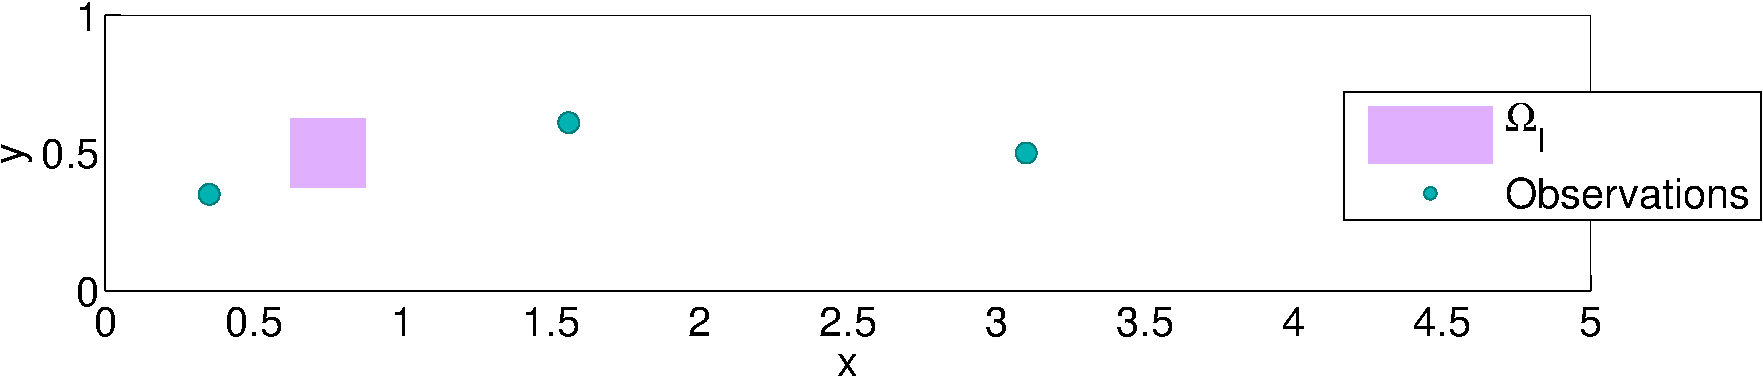
\includegraphics[width=0.8\textwidth]{baseSeries/setup_3_3.pdf}
\caption{Locations of the observations and the QoI region.}
\label{fig:baseSetup}
\end{figure}
%

For the numerical simulations, we use the finite element method (FEM), employing a continuous Galerkin formulation with Lagrange elements. We use the \texttt{libMesh} library~\cite{libMeshPaper} for the FEM calculations. 
%\red{The library offers easy calculation of adjoint systems, error estimates and subdomain restricted variables.}\footnote{But we don't use Libmesh's error estimates or restrict variables to subdomains...} 
The domain is discretized by a regular mesh of quadrilaterals, with 250 and 50 elements along the $x_1$ and $x_2$ directions, respectively, for a total of 12,500 elements, resulting in 12,801 degrees of freedom per variable. The diffusion coefficient is such that the cell P\'{e}clet number never exceeds 0.1, and thus no stabilization is required.
%
%------------------------------------------------------------%
\subsubsection{Adaptive Model Refinement Results} \label{sec:cdvcdrBaseRef} 
%------------------------------------------------------------%
%

We now present the results for solving the inference problem using \cref{alg:refSeries}. Once the QoI error estimate is calculated using \cref{eq:finErrExp}, the error estimate is then decomposed into local contributions. At each iteration, based on this decomposition, we choose the basis functions with the largest error contributions until an additional 5\% of the elements has been marked for refinement. This is repeated until the estimated absolute relative error in the QoI, calculated as $\epsilon_i/(\epsilon_i+I(q_{MF_i},u_{MF_i}))$, is less than $1\%$.

\Cref{fig:baseRef} shows the local error contributions, as well as the subdomains where the low- and high-fidelity models are used, for the series of mixed-fidelity models thus generated. Each linear Lagrange basis function's contribution is plotted at its nonzero node.
%
\begin{figure}[htbp]
%\captionsetup[subfloat]{captionskip=-5pt}
\centering
\subfloat[LF $\equiv$ MF$_0$ ($0\%$ HF)]{
  
\includegraphics[width=0.46\textwidth]{baseSeries/cd_cdr_LF_divvy.png}
  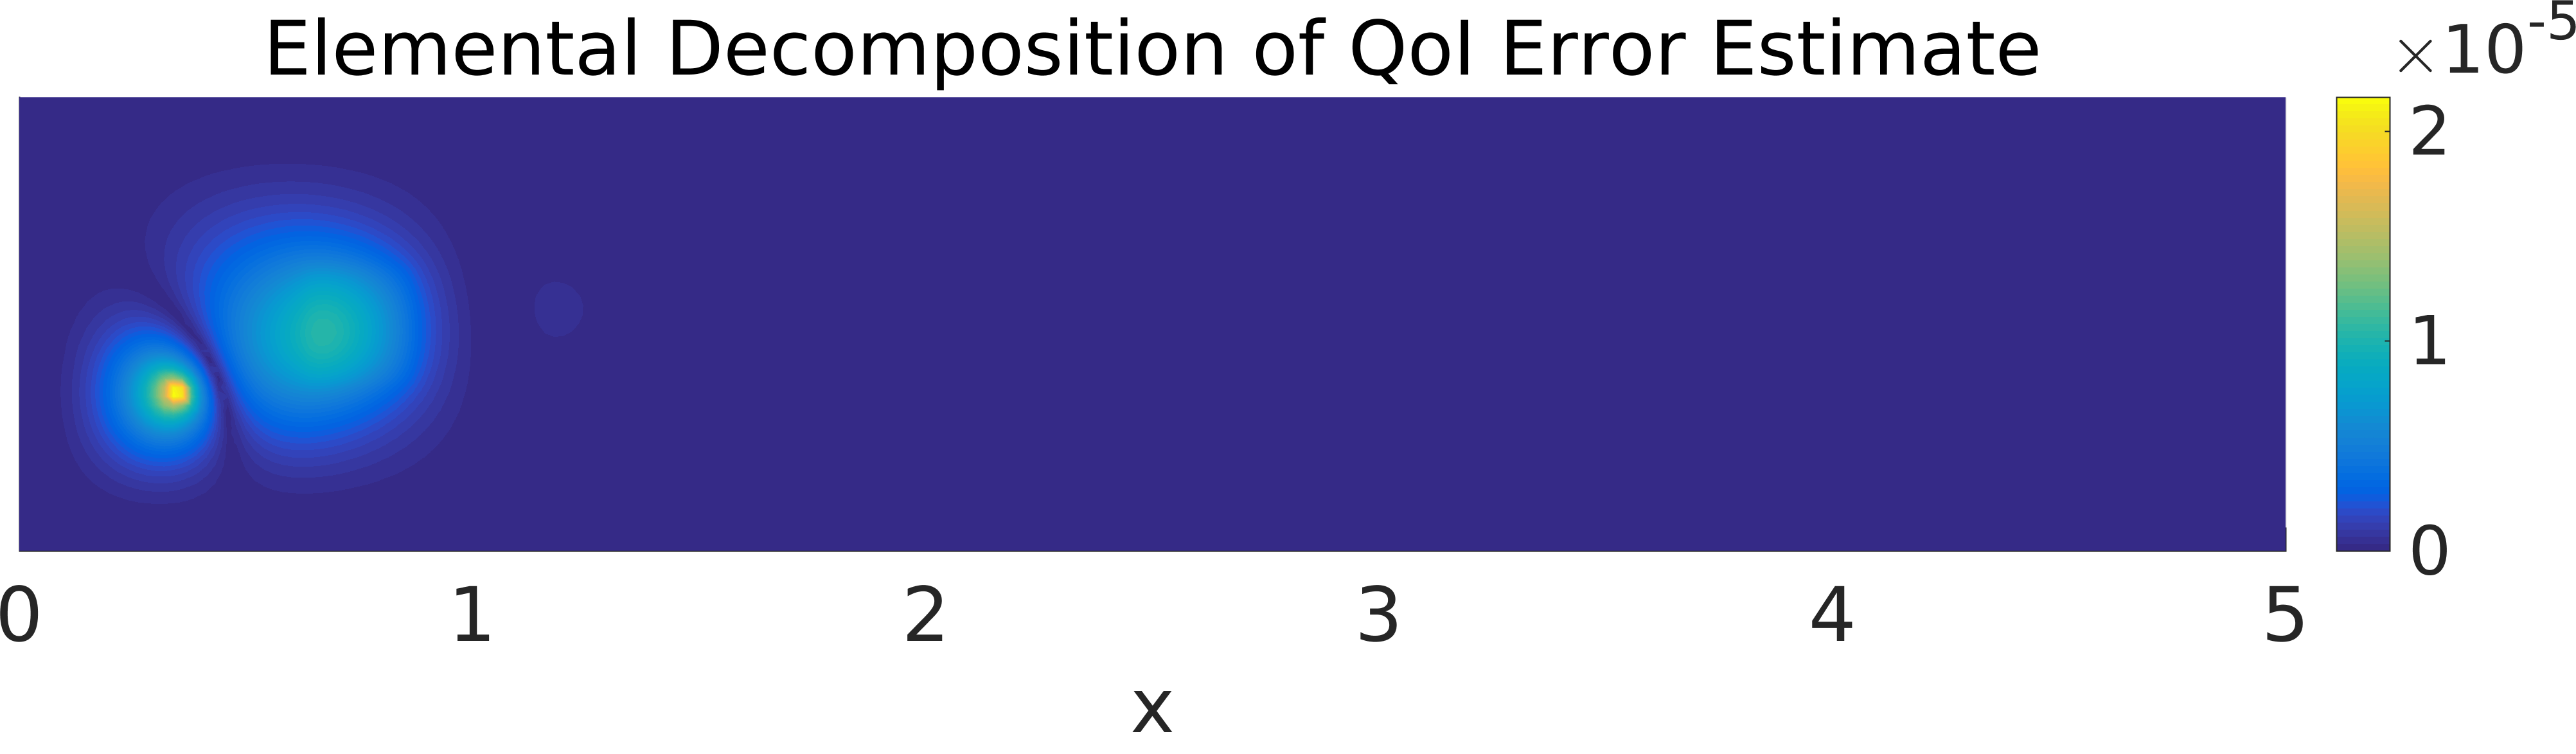
\includegraphics[width=0.49\textwidth]{baseSeries/err_breakdown_LF.png}
  \label{fig:baseRef0}
} \\
\subfloat[MF$_1$ ($5\%$ HF)]{
  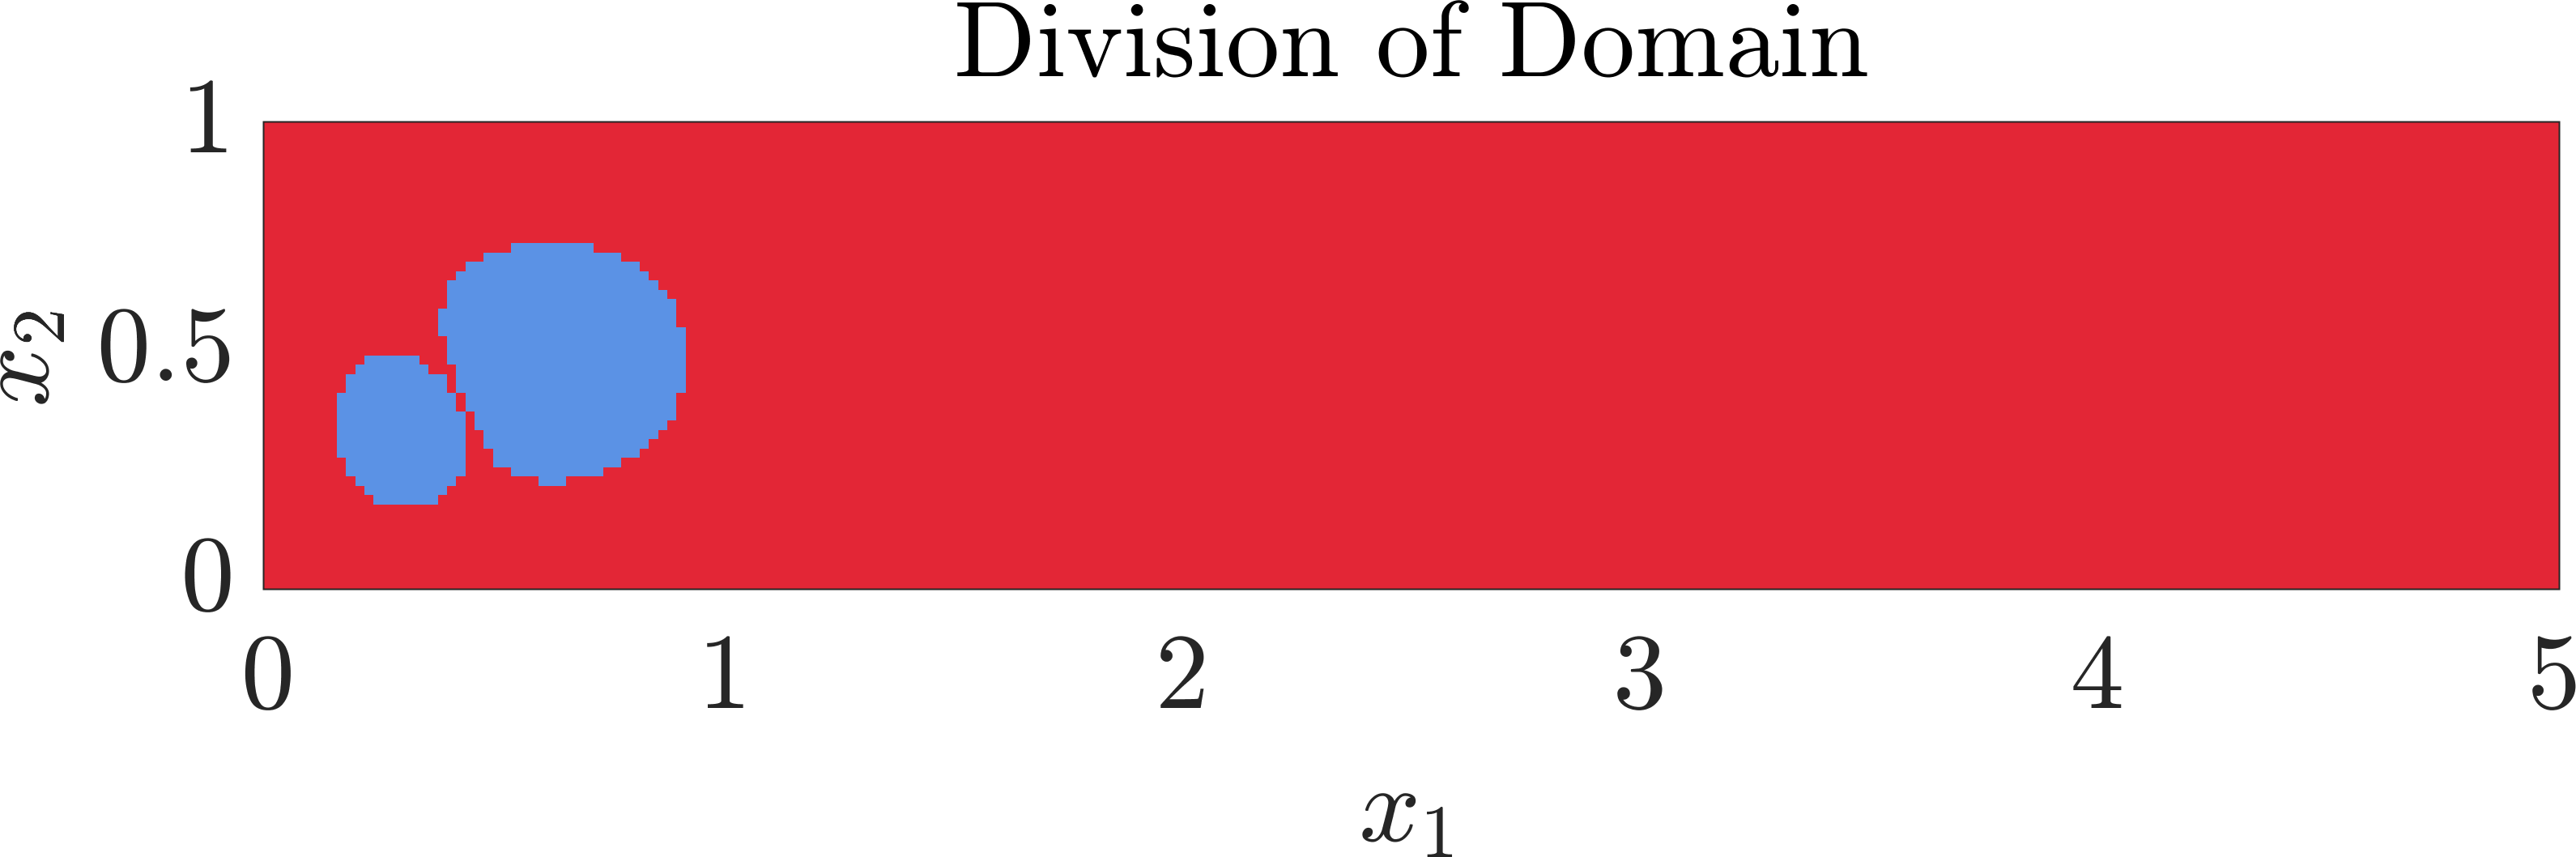
\includegraphics[width=0.46\textwidth]{baseSeries/cd_cdr_MF01_divvy.png}
  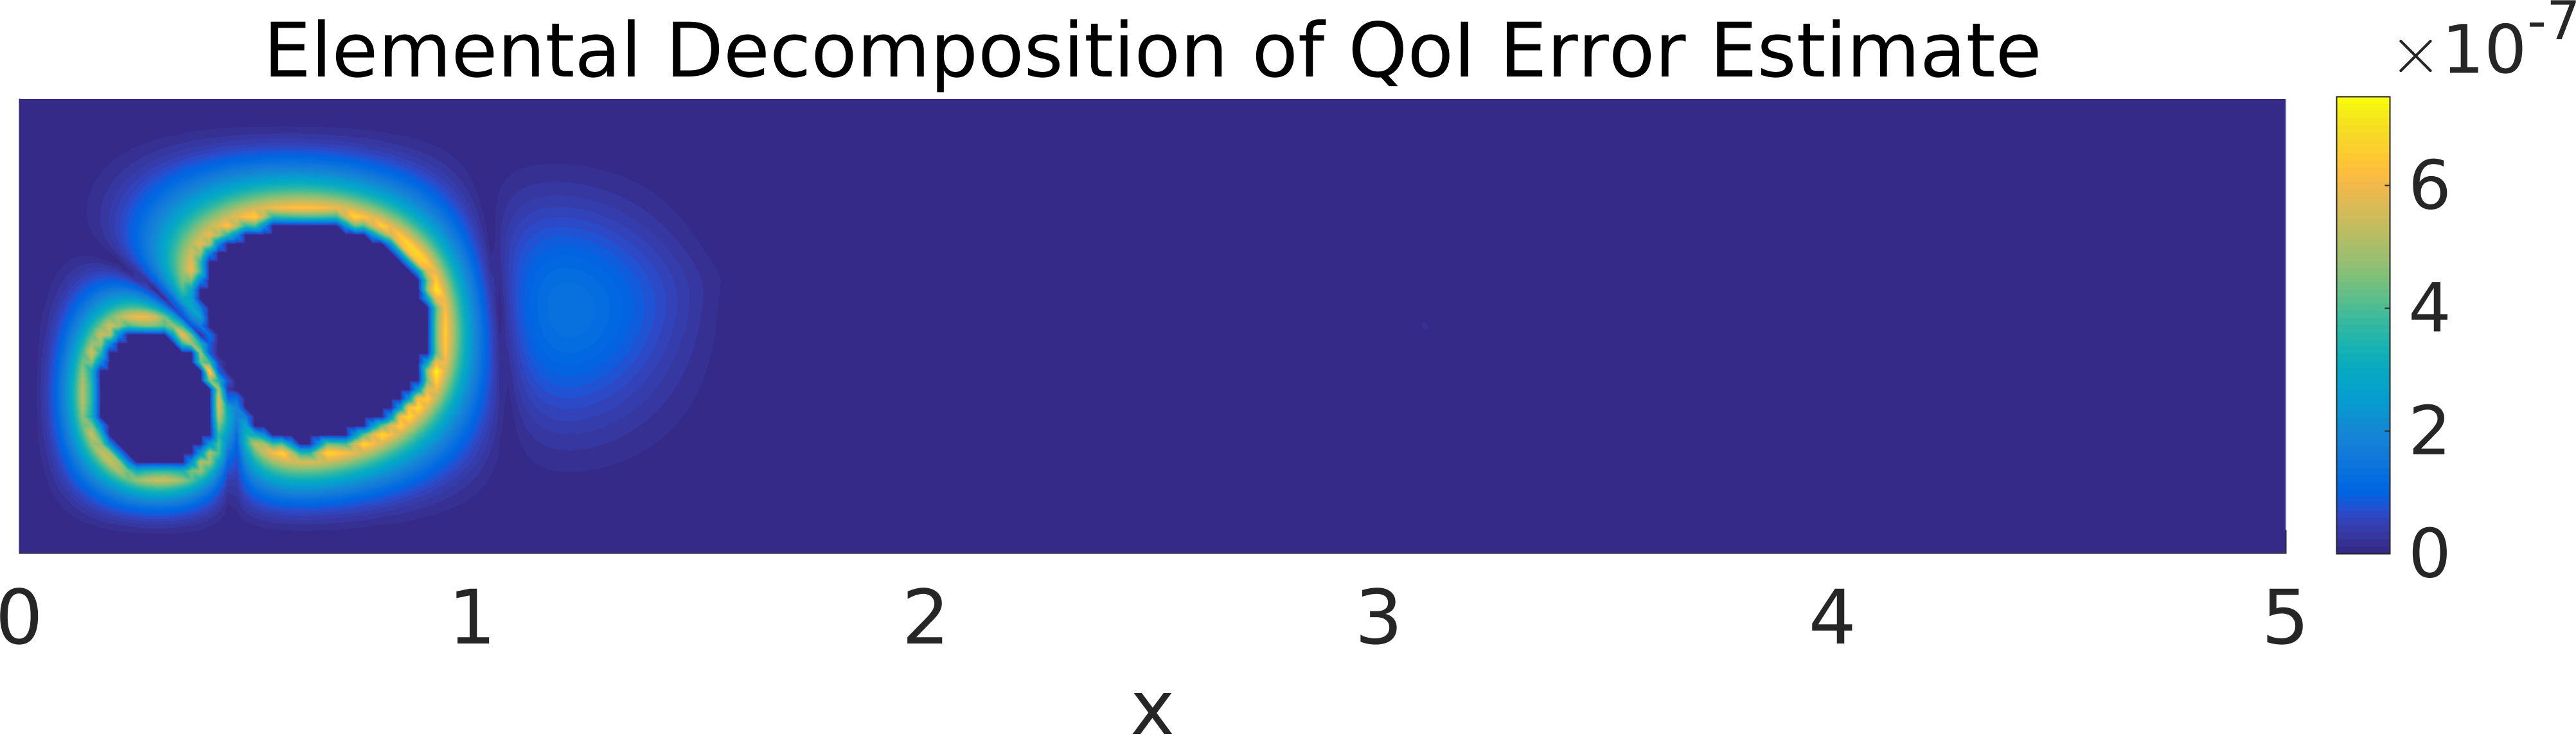
\includegraphics[width=0.49\textwidth]{baseSeries/err_breakdown_MF01.png}
} \\
\subfloat[MF$_2$ ($10\%$ HF)]{
  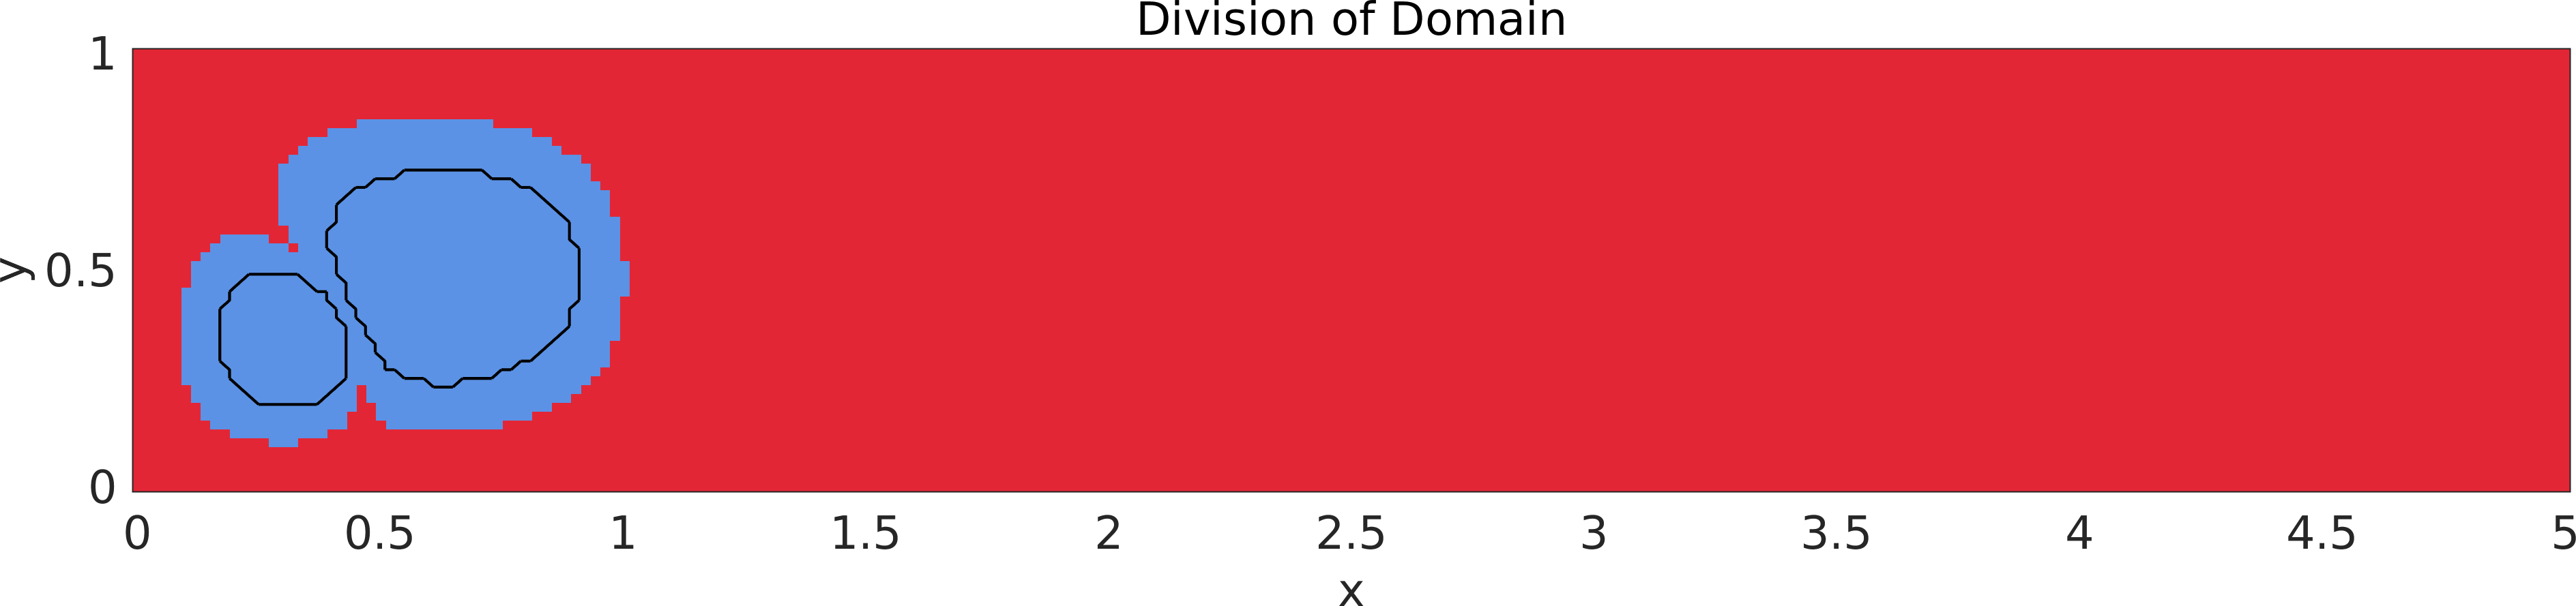
\includegraphics[width=0.46\textwidth]{baseSeries/cd_cdr_MF02_divvy.png}
  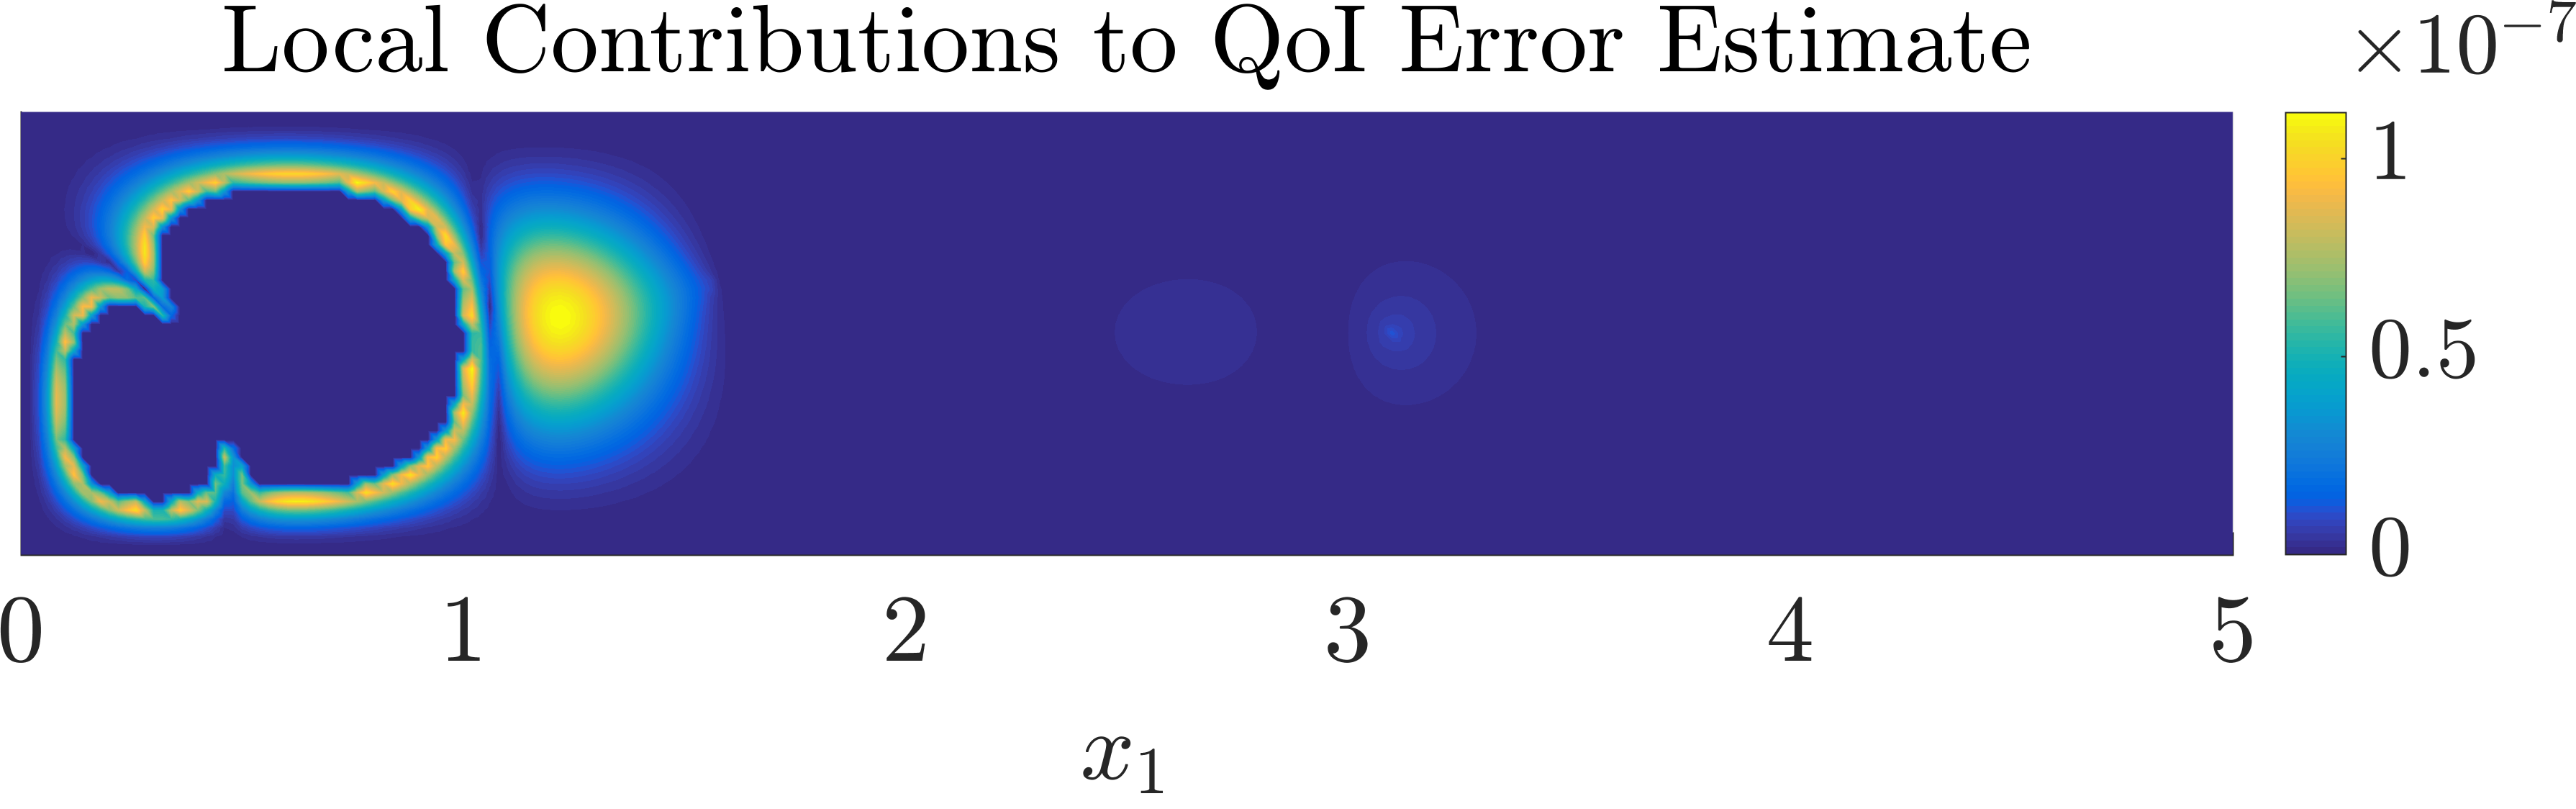
\includegraphics[width=0.49\textwidth]{baseSeries/err_breakdown_MF02.png}
} \\
\caption{Local error contributions (right) and domain division (left; low-fidelity convection-diffusion model used in red portion, high-fidelity convection-diffusion-reaction model used in blue portion) for mixed-fidelity models.}
\label{fig:baseRef}
\end{figure}
%
Note that the error contribution of each basis function whose support is entirely within the high-fidelity regions is zero.

We see that the largest local error contribution is concentrated in the QoI region, and the data point closest to the QoI. In the first decomposition of the error (\cref{fig:baseRef0}), the region where the elemental error is maximum is the leftmost data point. Since the constraining model is an elliptic PDE, with weak convection, information flow is localized, and is weakly convected from left to right. Therefore, for the calculation of the QoI, it is most important to refine the region near the leftmost data point, and the QoI region. After that, the error decomposition suggests refinement in regions upstream and around the middle data point, and then the rightmost data point.

\Cref{fig:baseErr} shows the true and estimated absolute relative errors in the QoI for the various mixed-fidelity models generated by \cref{alg:refSeries}; the true and estimated relative errors are calculated relative to the true and estimated high-fidelity QoI, respectively. In this case, we see that QoI error of $1\%$ is attained with a mixed-fidelity model where the high-fidelity model is used in only about $10\%$ of the domain. We note that, in general, there is no guarantee that either the error in the QoI or the relative error in the error estimate will decrease monotonically as more of the domain is refined.
%
\begin{figure}[htbp]
\centering
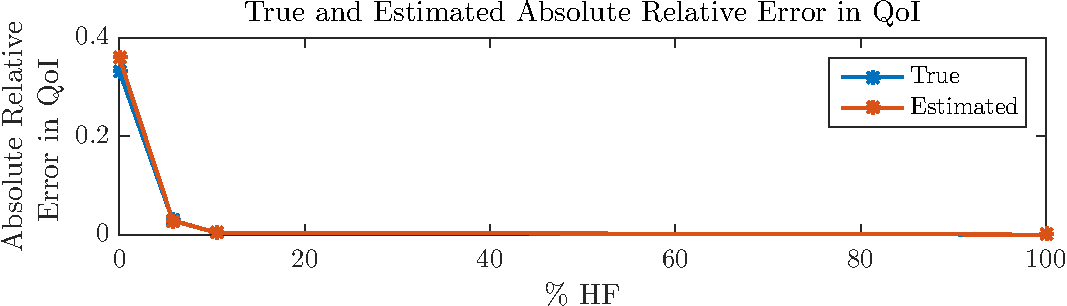
\includegraphics[width=0.8\textwidth]{baseSeries/err_est.pdf}
\caption{True and estimated absolute relative error in QoI, plotted as a function of the percentage area of the domain in which the high-fidelity convection-diffusion-reaction model is used.}
\label{fig:baseErr}
\end{figure}
%

%------------------------------------------------------------%
\subsubsection{Interaction of Observations and QoI} \label{sec:qoivdata}
%------------------------------------------------------------%
%
The error estimate decomposition suggests the use of the high-fidelity model in areas of the domain that are important to the interaction between the observations and QoI; the interaction between these two can be complex, and the areas suggested for refinement may be nonintuitive. To see this, we compare the error estimate decomposition for three sizes of the QoI region $\Omega_I$ given the same set of data points, and for three nested sets of data points given the same QoI region. For the sake of illustration, we make two refinement iterations for each combination of observations and QoI region, regardless of the magnitude of the relative error estimate. However, it was noticed that the number of iterations needed to achieve a given tolerance increased as the QoI region increased.

The error decompositions for three increasingly large, nested QoI regions $\Omega_I$ given the same set of observations are shown in \cref{fig:qoiStudy}. The bottom row gives the baseline case presented in \cref{sec:cdvcdrBaseRef}, although here we choose the basis functions $i$ whose error $\varepsilon_i$ are among the largest $5\%$, so the proportion of additional refined elements in each iteration is slightly larger. Although refinement is still most important around the data point closest to $x_1=0$, as the QoI region expands the other two data points become more important in that the error decomposition suggests refinement around them earlier. As the QoI region expands, it is also more clearly noticeable that refinement is not equally important in all parts of the QoI region.

\begin{figure}[htbp]
\centering
\subfloat[Locations of observations and QoI region $\Omega_I$][Locations of \\observations and \\QoI region $\Omega_I$]{
  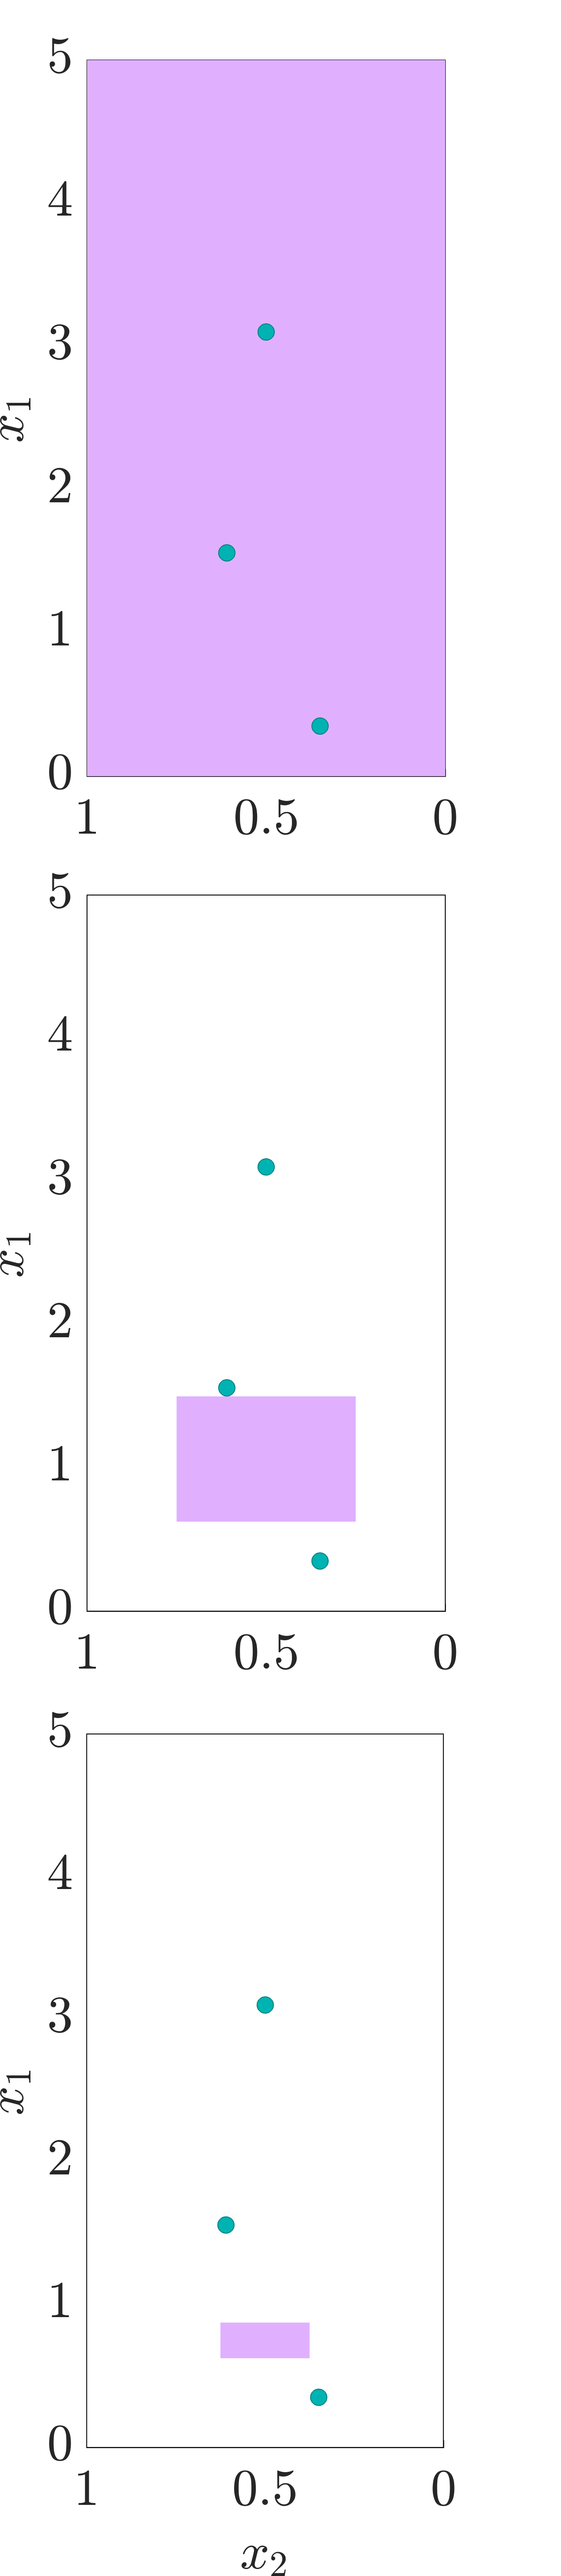
\includegraphics[width=0.23\textwidth]{vs_qoi/vs_qoi_setup.png}
  \label{subfig:obsSetup}
}
\subfloat[MF$_0$ ($0\%$ HF)][MF$_0$ \\($0\%$ HF)]{
  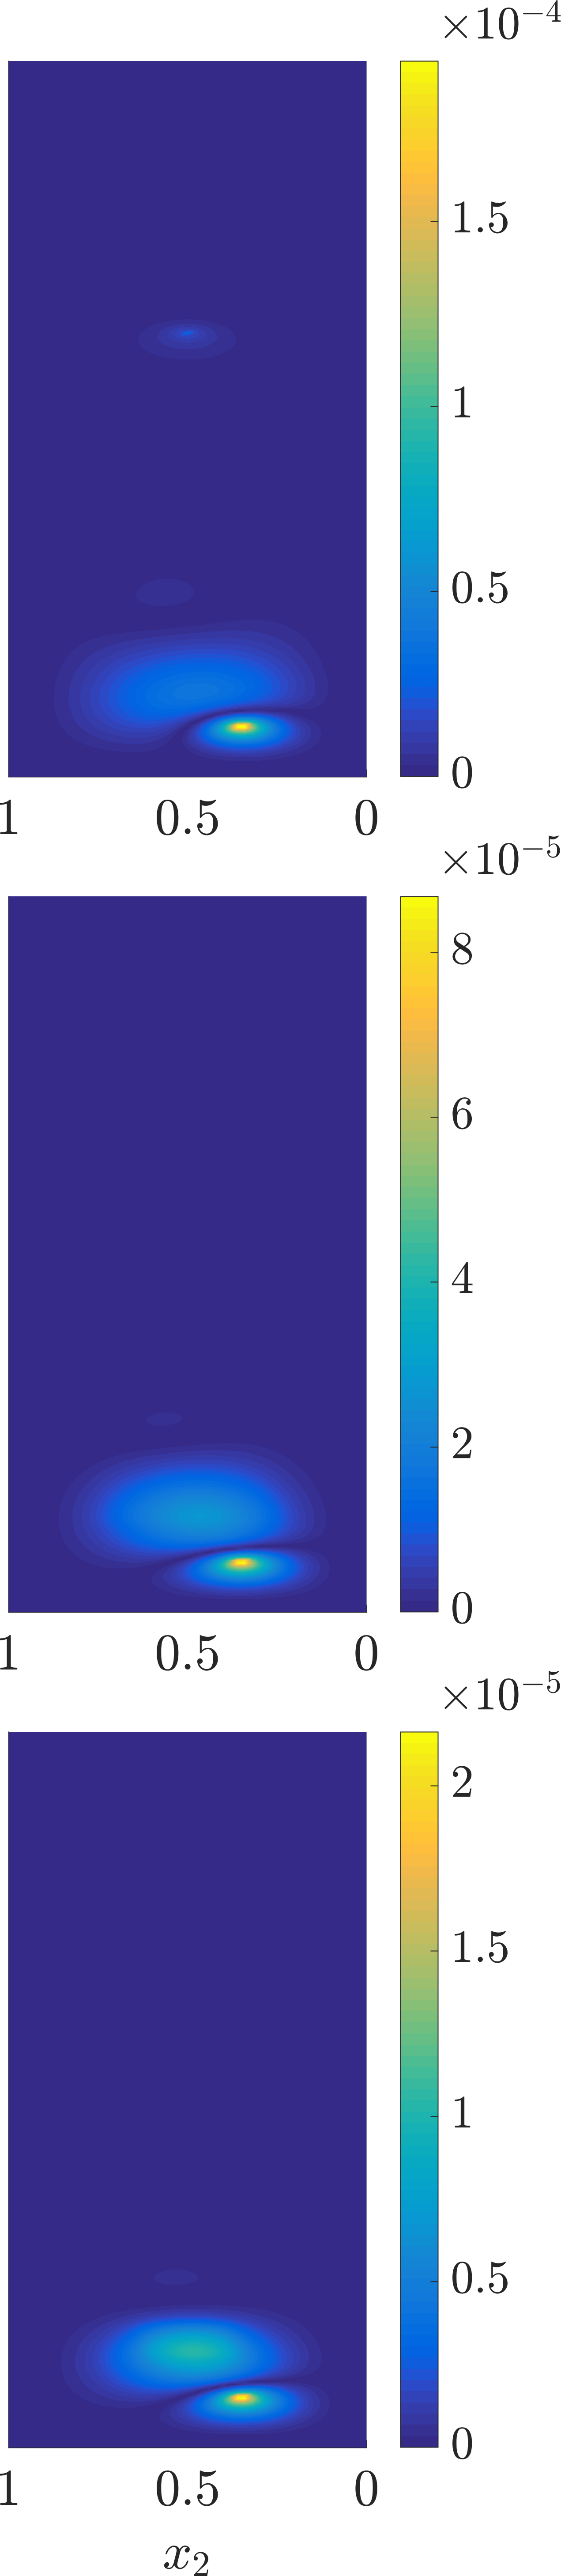
\includegraphics[width=0.23\textwidth]{vs_qoi/vs_qoi_err0.png}
  \label{subfig:obsLF}
}
\subfloat[MF$_1$ ($\sim5\%$ HF)][MF$_1$ \\($\sim5\%$ HF)]{
  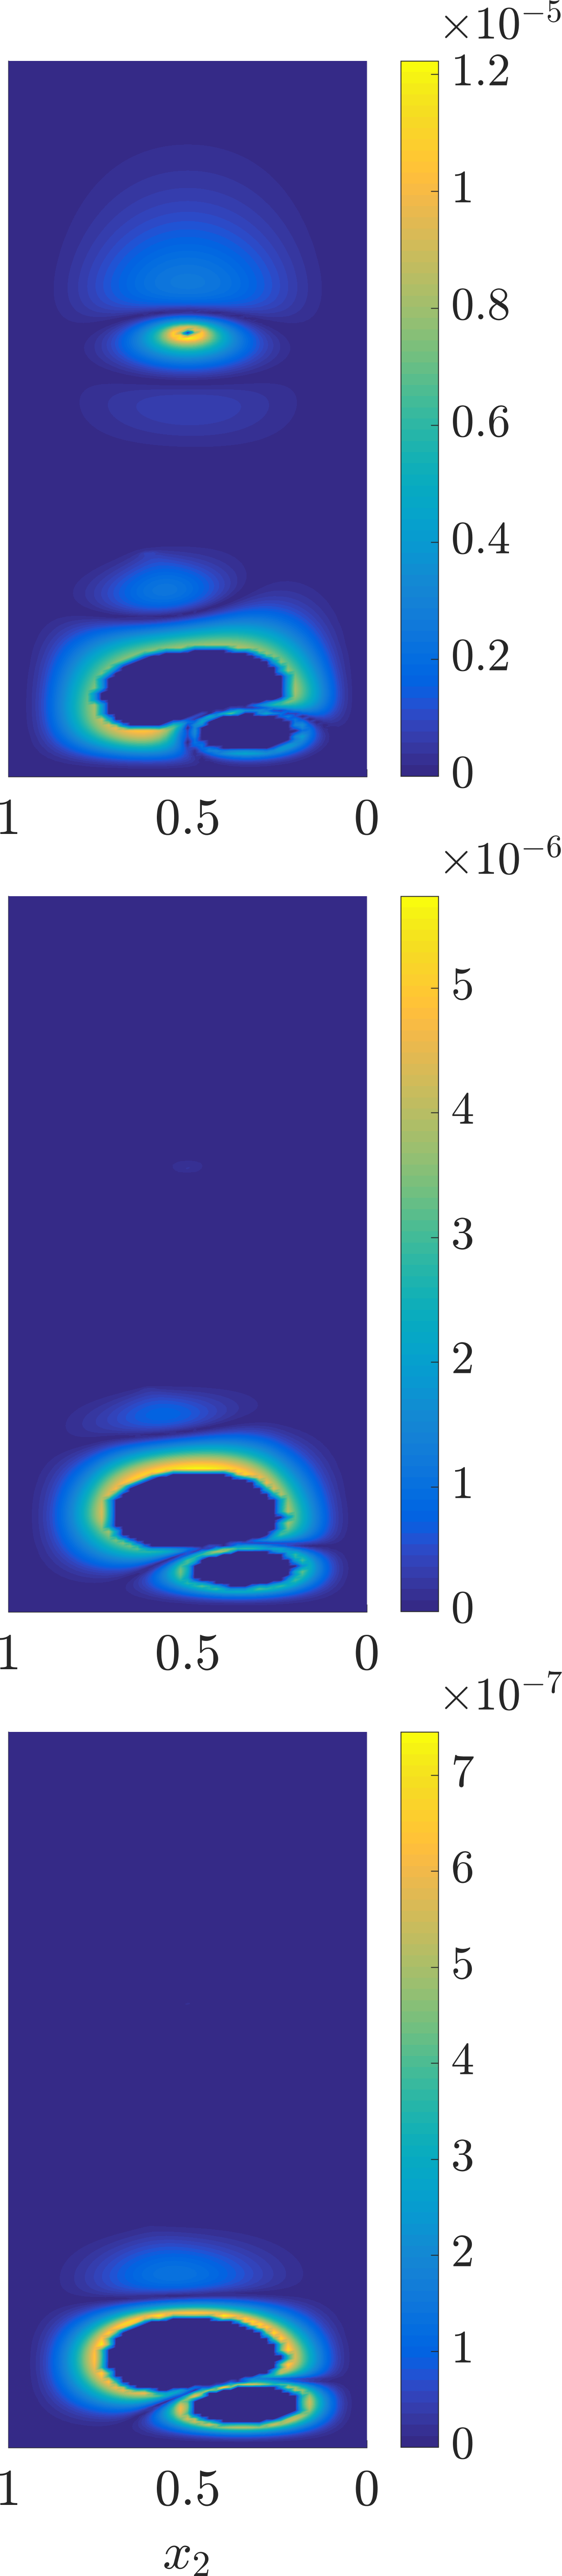
\includegraphics[width=0.23\textwidth]{vs_qoi/vs_qoi_err1.png}
}
\subfloat[MF$_2$ ($\sim10\%$ HF)][MF$_2$ \\($\sim10\%$ HF)]{
  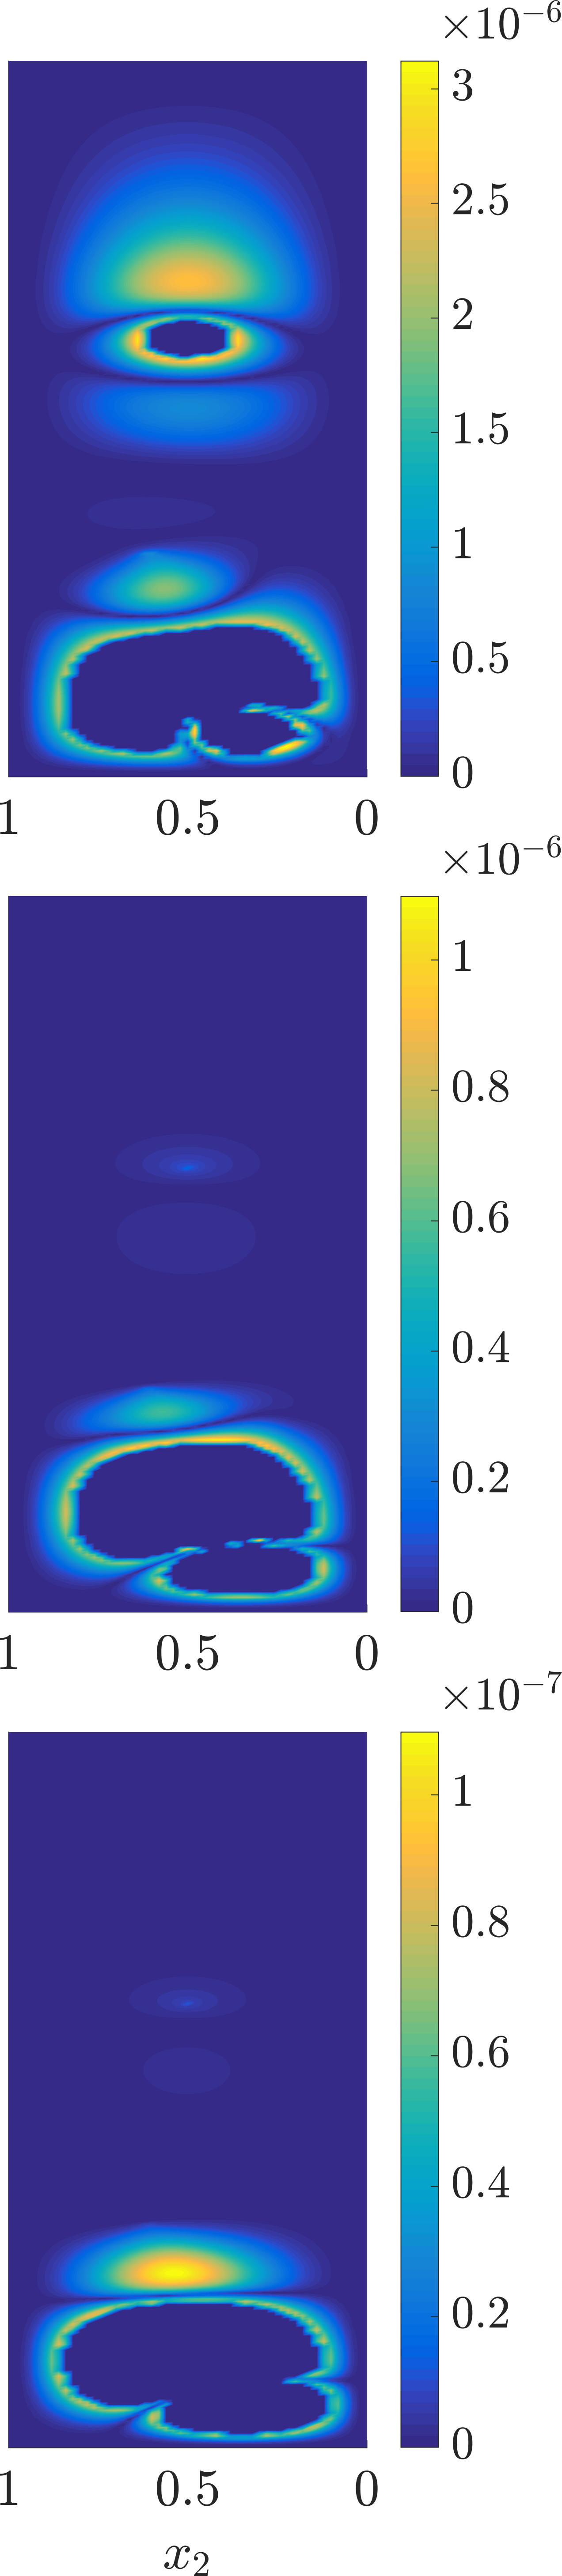
\includegraphics[width=0.23\textwidth]{vs_qoi/vs_qoi_err2.png}
  \label{subfig:obsMFlast}
}
  \caption{With each row corresponding to the configuration of observations (teal points) and QoI region (purple box) shown in column \protect\subref{subfig:obsSetup}, compare the error estimate decompositions (columns \protect\subref{subfig:obsLF}-\protect\subref{subfig:obsMFlast}) given the same observations and different QoI regions.}
  \label{fig:qoiStudy}
\end{figure}

The error decomposition for three increasing, nested sets of observations and the same QoI region $\Omega_I$ is shown in \cref{fig:dataStudy}. Again, the bottom row gives the baseline case presented in \cref{sec:cdvcdrBaseRef}, although here the basis functions with the largest $5\%$ of the error are chosen, so the proportion of additional refined elements in each iteration is slightly larger. Refinement appears to be consistently most important around the data point closest to $x_1=0$ and the QoI region. However, as more data points are added, it becomes no longer necessarily true that refinement becomes less important around data points as their distance from the QoI region increases. The data points also interact with each other in that placing data points in regions of previously relatively uniform error contribution tends to result in a new error decomposition that is positive or negative around the data points, with valleys of zero magnitude in between.

\begin{figure}[htbp]
\centering
\subfloat[Locations of observations and QoI region $\Omega_I$][Locations of \\observations and \\QoI region $\Omega_I$]{
  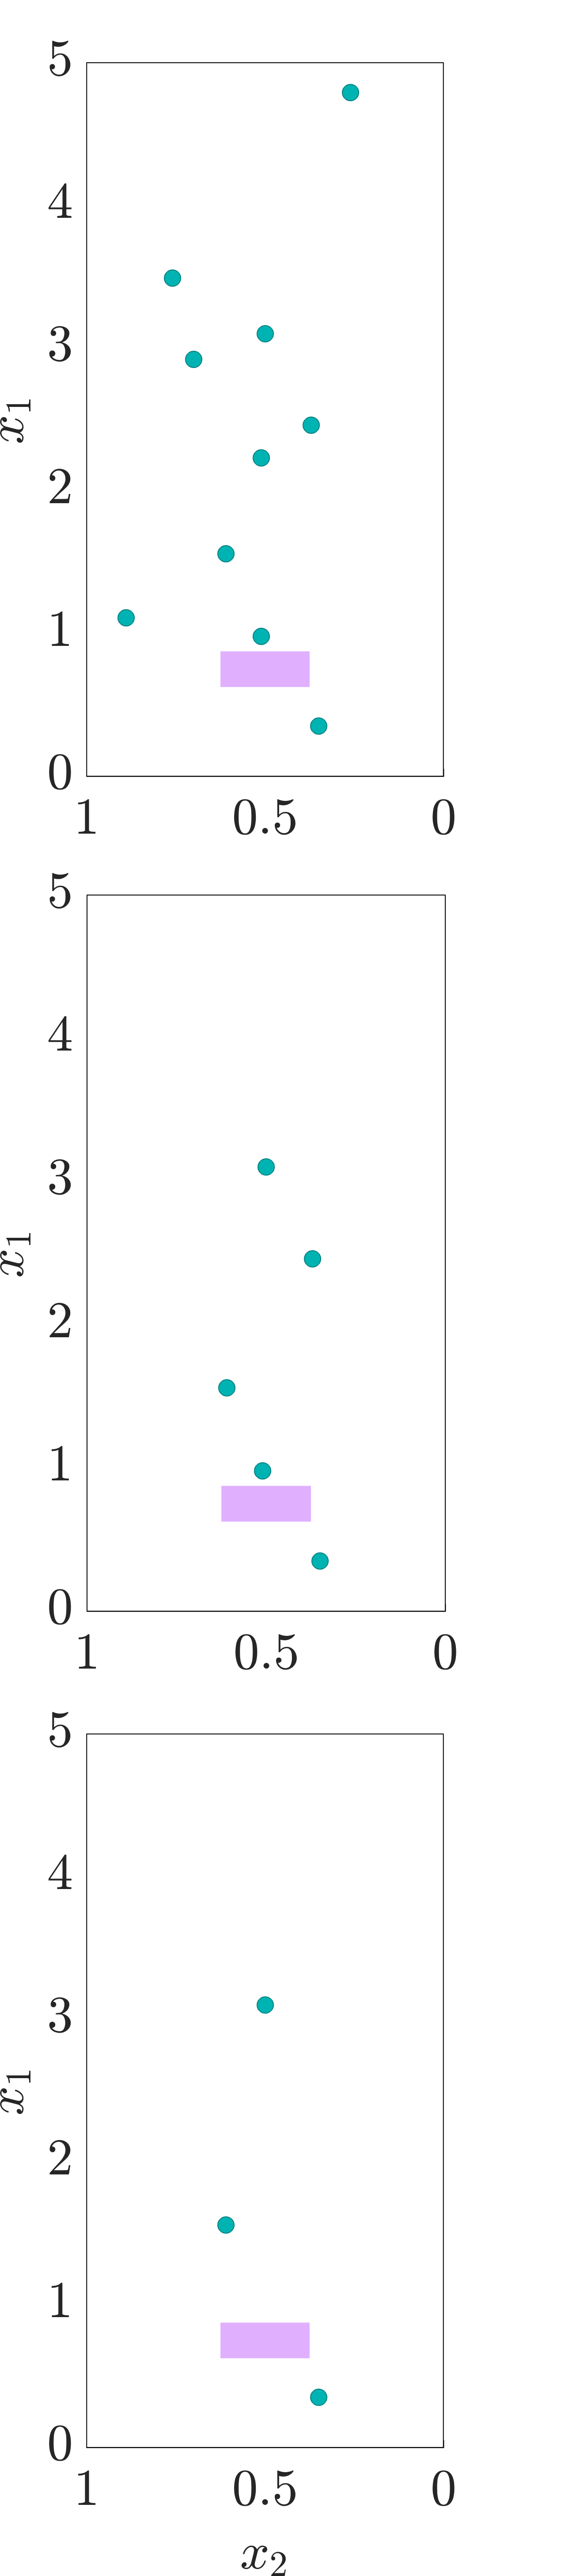
\includegraphics[width=0.23\textwidth]{vs_data/vs_data_setup.png}
  \label{subfig:obsSetup2}
} 
\subfloat[MF$_0$ ($0\%$ HF)][MF$_0$ \\($0\%$ HF)]{
  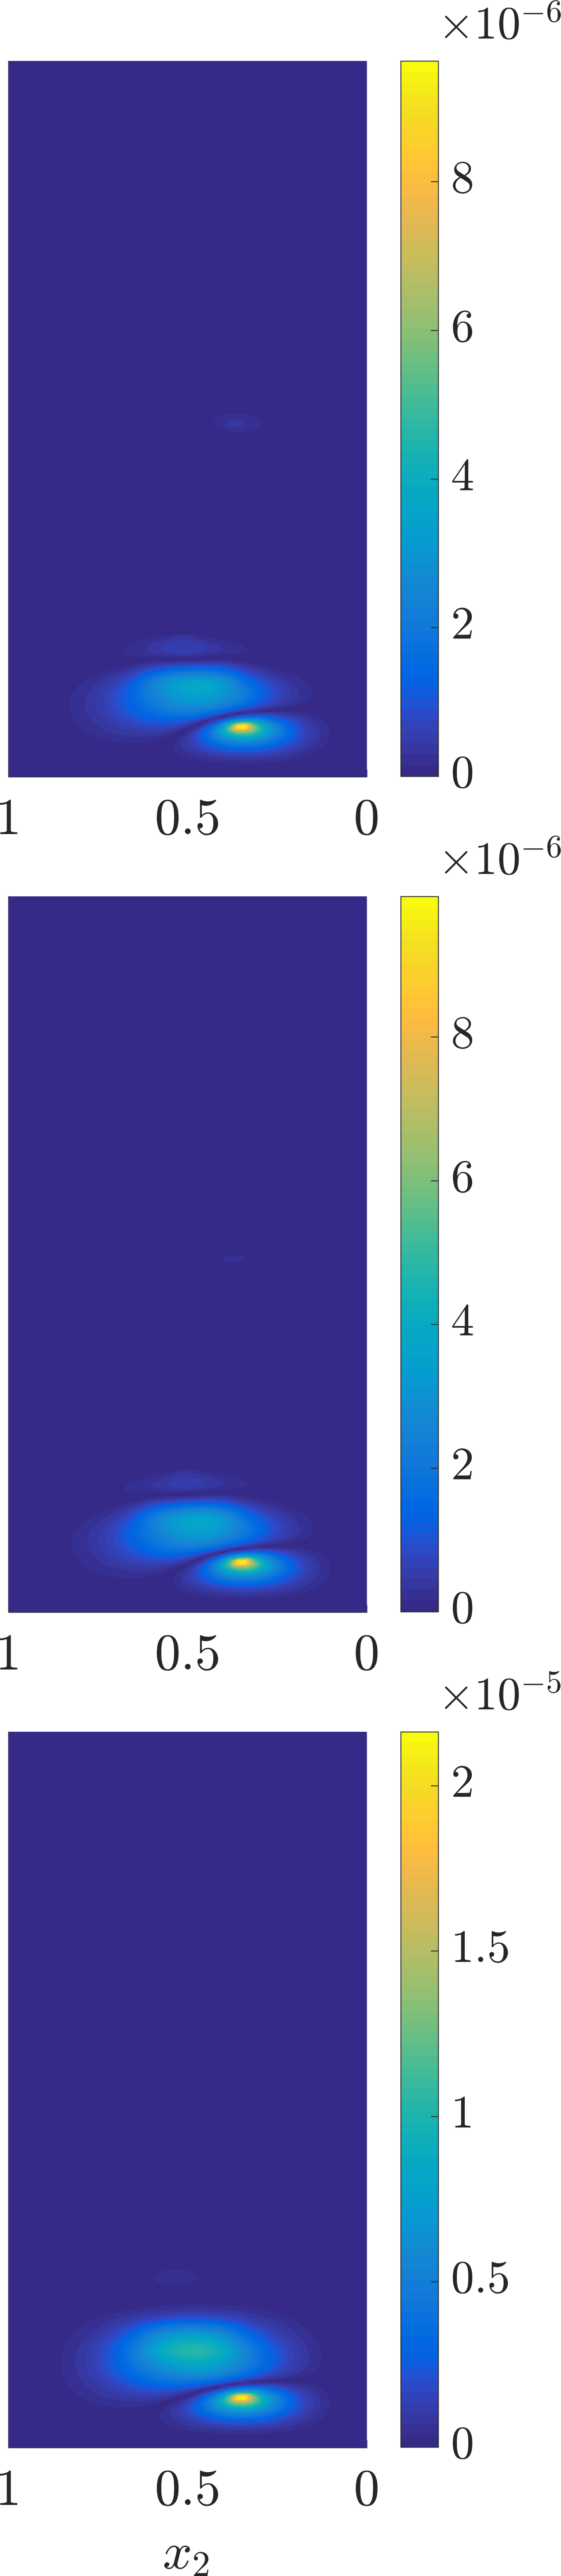
\includegraphics[width=0.23\textwidth]{vs_data/vs_data_err0.png}
  \label{subfig:obsLF2}
}
\subfloat[MF$_1$ ($\sim5\%$ HF)][MF$_1$ \\($\sim5\%$ HF)]{
  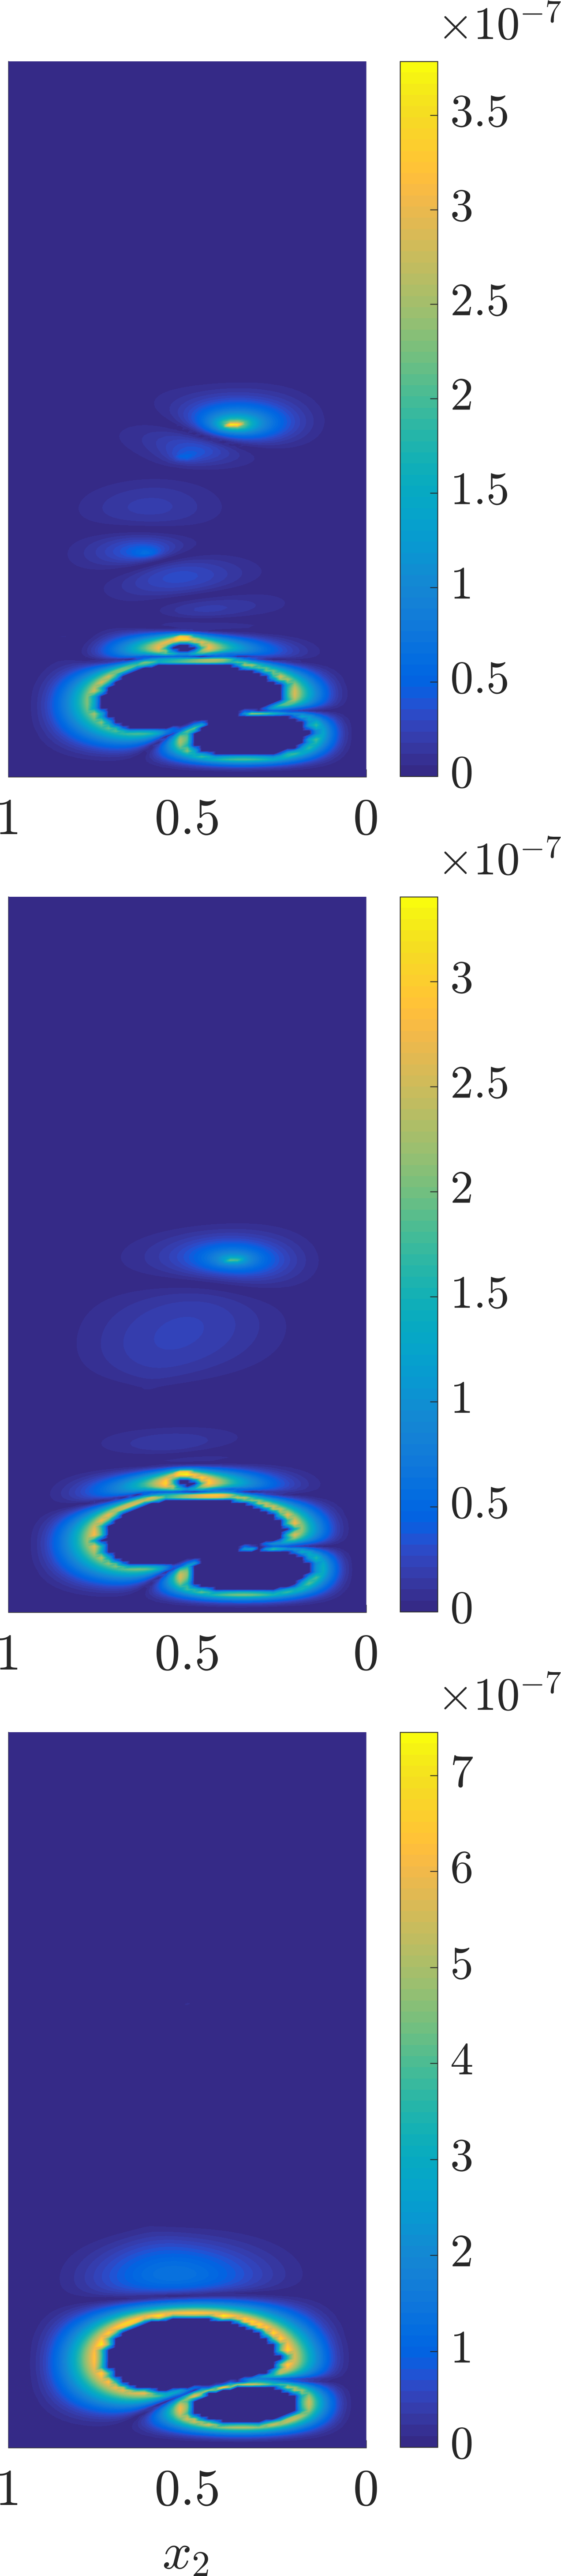
\includegraphics[width=0.23\textwidth]{vs_data/vs_data_err1.png}
}
\subfloat[MF$_2$ ($\sim10\%$ HF)][MF$_2$ \\($\sim10\%$ HF)]{
  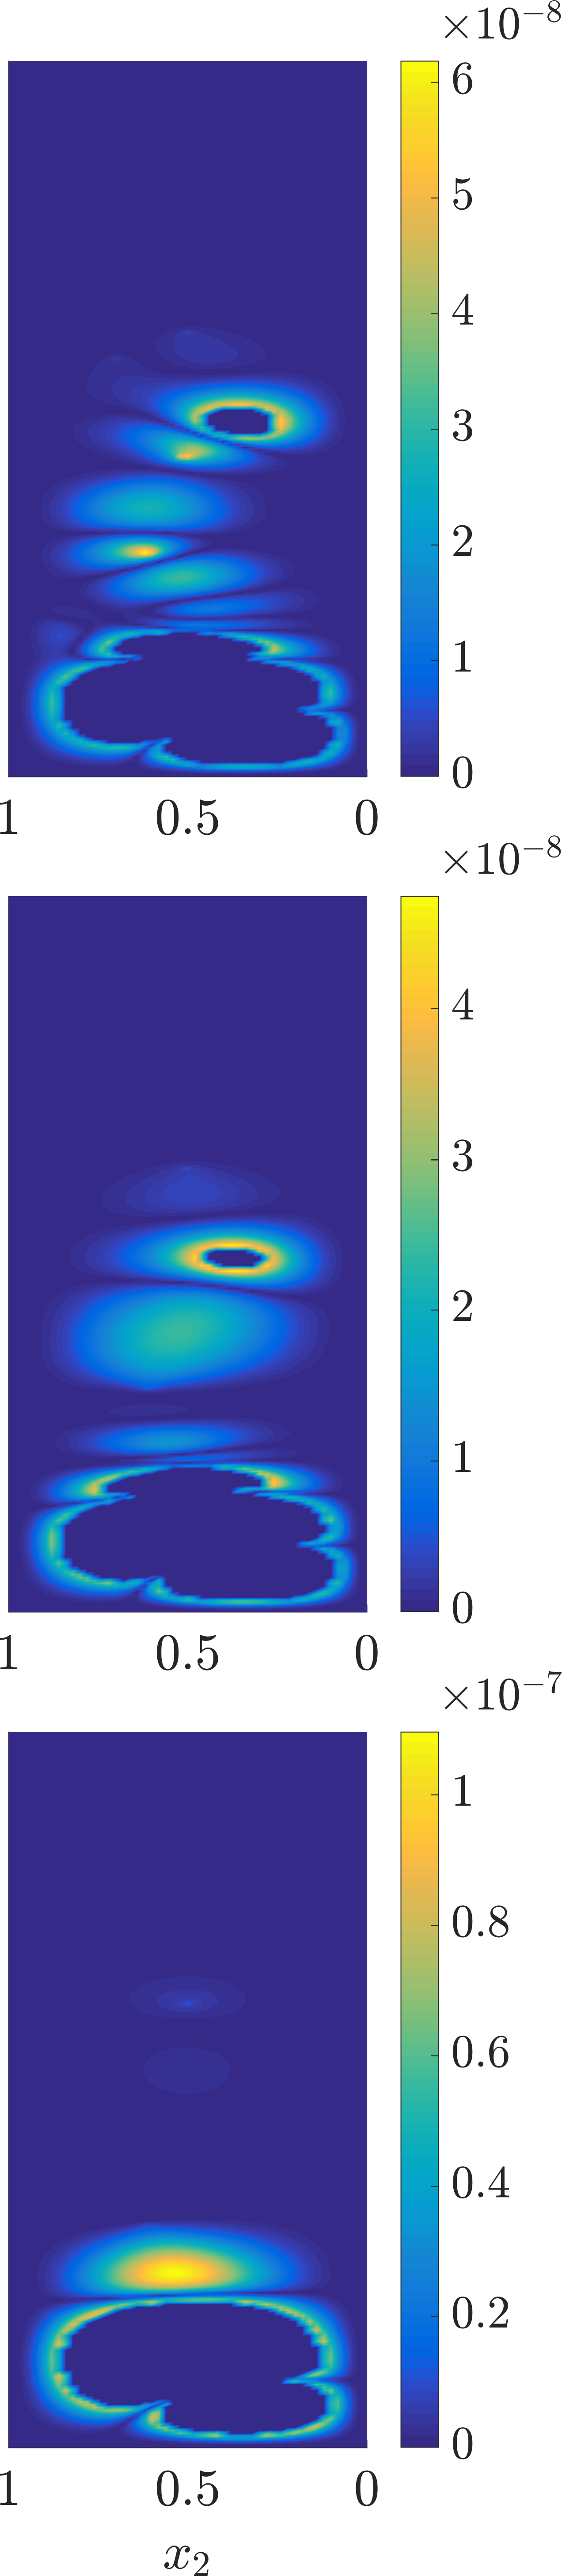
\includegraphics[width=0.23\textwidth]{vs_data/vs_data_err2.png}
  \label{subfig:obsMFlast2}
}
  \caption{With each row corresponding to the configuration of observations (teal points) and QoI region (purple box) shown in column \protect\subref{subfig:obsSetup2}, compare the error estimate decompositions (columns \protect\subref{subfig:obsLF2}-\protect\subref{subfig:obsMFlast2}) given different observations and the same QoI region.}
  \label{fig:dataStudy}
\end{figure}

%------------------------------------------------------------------------------------------------------------------------%
\subsection{Constant vs Field Parameters} \label{sec:constvfield}
%------------------------------------------------------------------------------------------------------------------------%
\red{THIS SUBSECTION IS OLD AND CURRENTLY A PLACEHOLDER TO GAUGE LENGTH}. It is not necessary for the low- and high-fidelity models to differ in the physics included. A low-fidelity model may be more computationally tractable due to a reduced number of degrees of freedom rather than reduced nonlinearity. In this section, we consider two models which differ in the space to which the parameter belongs, with the low-fidelity model having fewer degrees of freedom.
%------------------------------------------------------------%
\subsubsection{Problem Setup}
%------------------------------------------------------------%
We consider the same high-fidelity model as in \cref{sec:cdvcdr}:
\begin{equation}
k_d\nabla^2 u - \vec{V}\cdot\nabla u + k_ru^2= f(q),\quad q\in U,
\end{equation}
with the same diffusion coefficient $k_d = 0.1$  and reaction coefficient $k_r = -42$. The low-fidelity model
\begin{equation}
k_d\nabla^2 u - \vec{V}\cdot\nabla u + k_ru^2= f(q),\quad q\in\R
\end{equation}
differs from the high-fidelity model only in that the parameter $q$ is a constant instead of a field. Then the intermediate mixed-fidelity models have parameter fields which are non-constant in only portions of the domain. For ease of implementation, we require that the resulting parameter field remain continuous at the interface between the low-fidelity and high-fidelity subdomains, although this constraint is not necessary for the theory to hold. The domain, mesh, boundary conditions, and velocity field, as well as the observations, unknown parameters to be inferred, and QoI, remain the same as described in \cref{sec:cdvcdr}. As the inverse problem is ill-posed, except for perhaps in the case where the low-fidelity model is used throughout the domain, regularization is added; the Tikhonov regularization term is $\frac{\beta}{2}\int_\Omega \|\nabla f(q)\|_2^2+f(q)^2\:\textrm{d}A$, where $\beta=10^{-3}$ is a regularization coefficient.

Although using such a pair of models has similarities to the problem of adaptive mesh refinement, we note that in this example only the parameter field changes in its level of refinement, not the state. Should the two models differ in the resolution of the state variables instead of the parameters, it is more efficient to use the approach discussed in \cite{BecVex05}.
%------------------------------------------------------------%
\subsubsection{Adaptive Model Refinement Results}
%------------------------------------------------------------%
As with the previous examples in \cref{sec:cdvcdr}, the decomposition of the error estimate is used to select additional regions of the domain in which to use the high-fidelity model. The number of degrees of freedom in the inverse problem increases with the proportion of the domain in which the high-fidelity model is used and the unknown parameter allowed to be a field. With each iteration, an additional $10\%$ of the elements are marked for refinement. This is repeated until the estimated absolute relative error in the QoI, is less than $1\%$.

\Cref{fig:svfRef} shows the local error contributions, as well as the subdomains where the low- and high-fidelity models are used, for the first two and last mixed-fidelity model thus generated. Each linear Langrange basis function's contribution is plotted at its nonzero node. 
%
\begin{figure}[htbp]
\centering
\subfloat[MF$_0$ ($0\%$ HF)]{
	
\includegraphics[width=0.46\textwidth]{svf/cd_cdr_LF_divvy.png}
  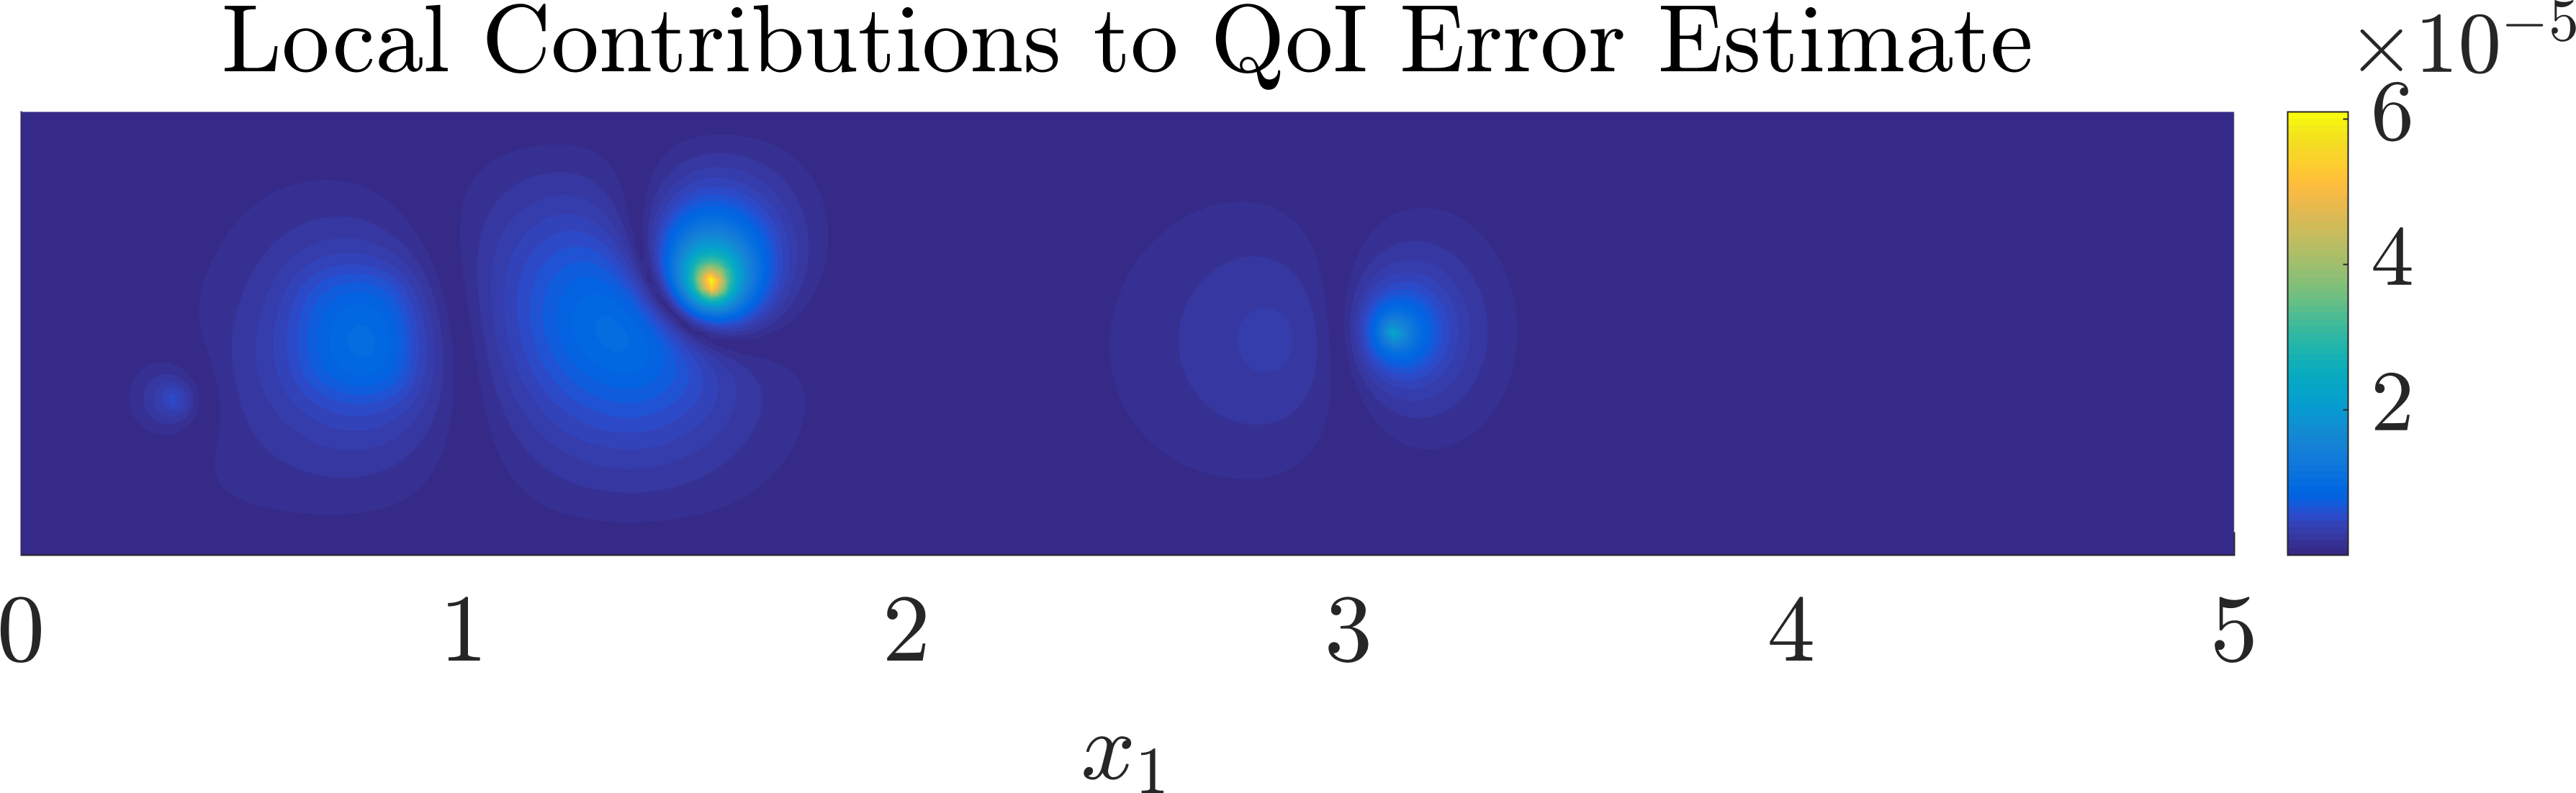
\includegraphics[width=0.49\textwidth]{svf/err_breakdown_LF.png}
} \\
\subfloat[MF$_1$ ($10\%$ HF)]{
	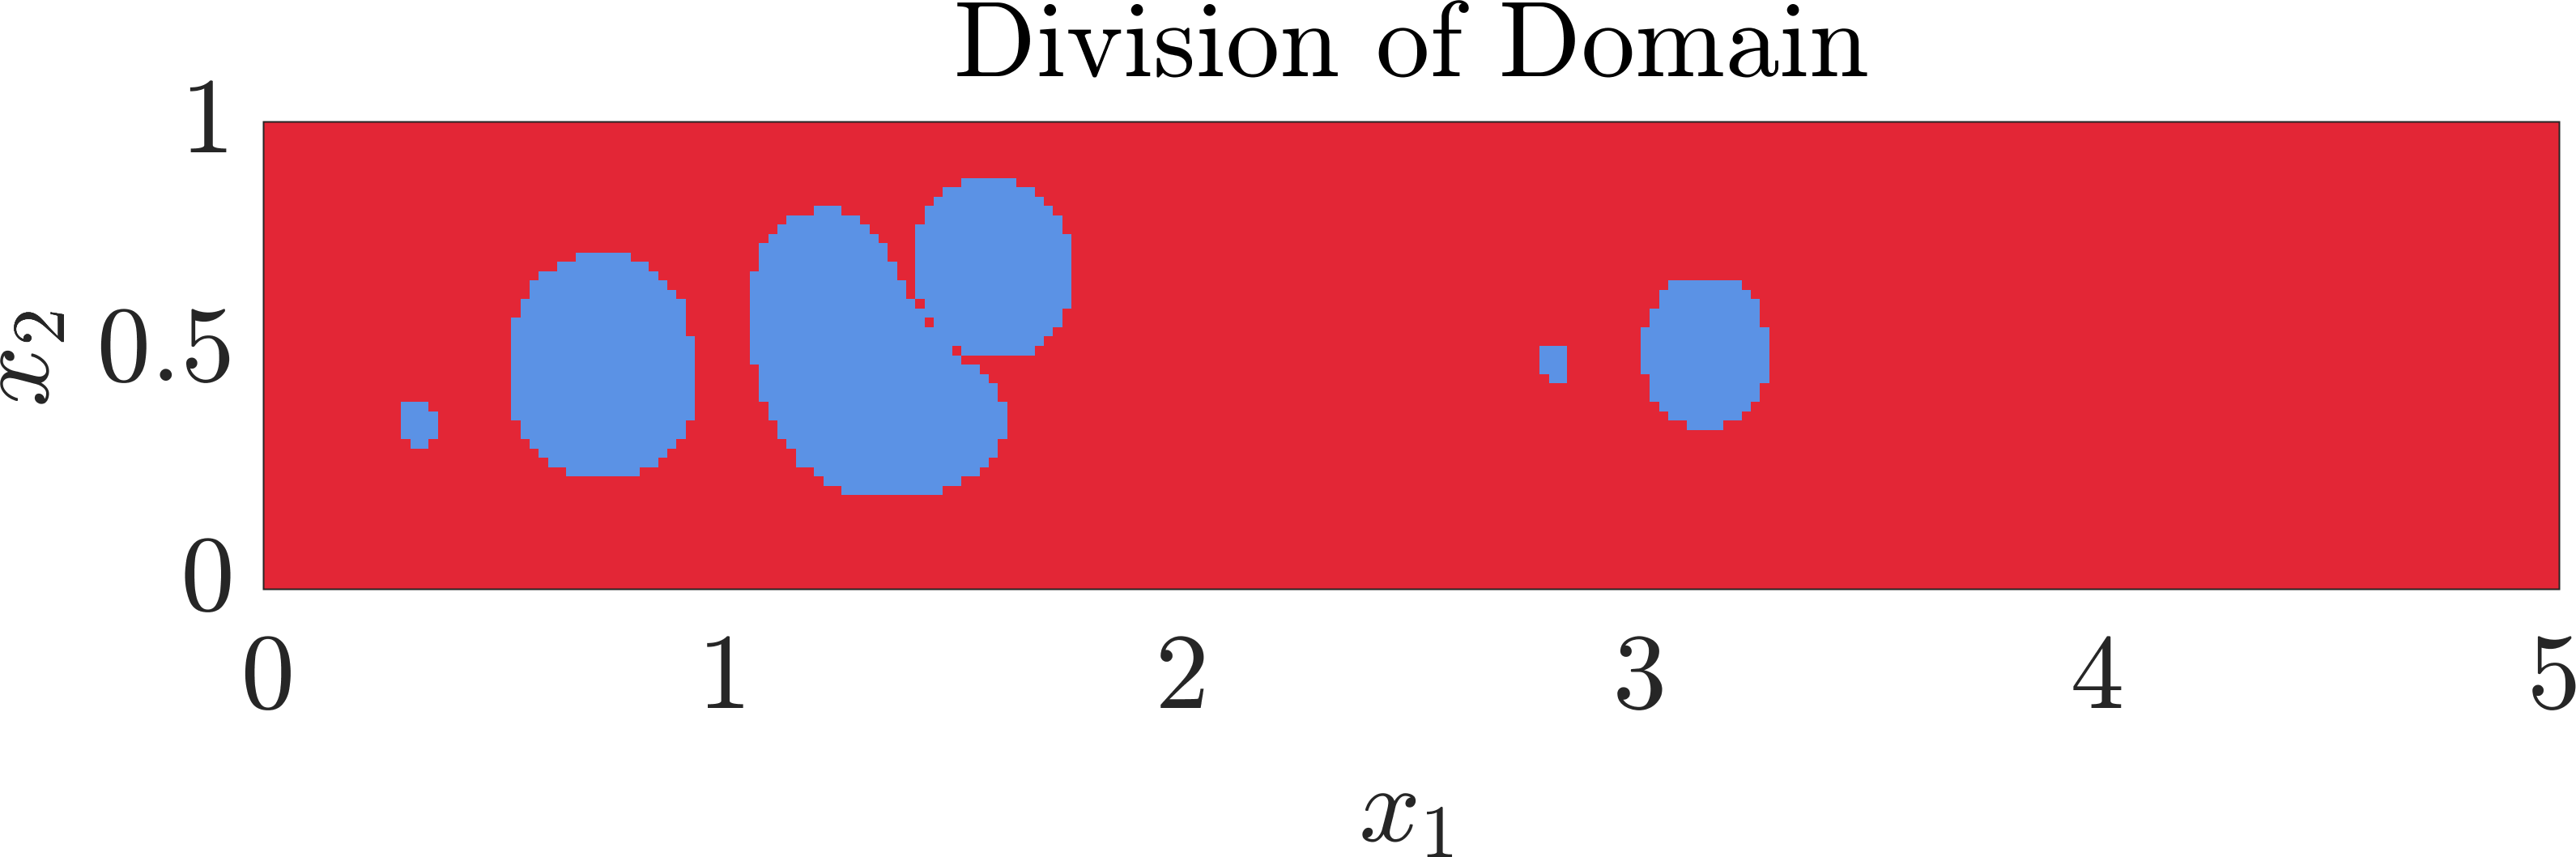
\includegraphics[width=0.46\textwidth]{svf/cd_cdr_MF01_divvy.png}
  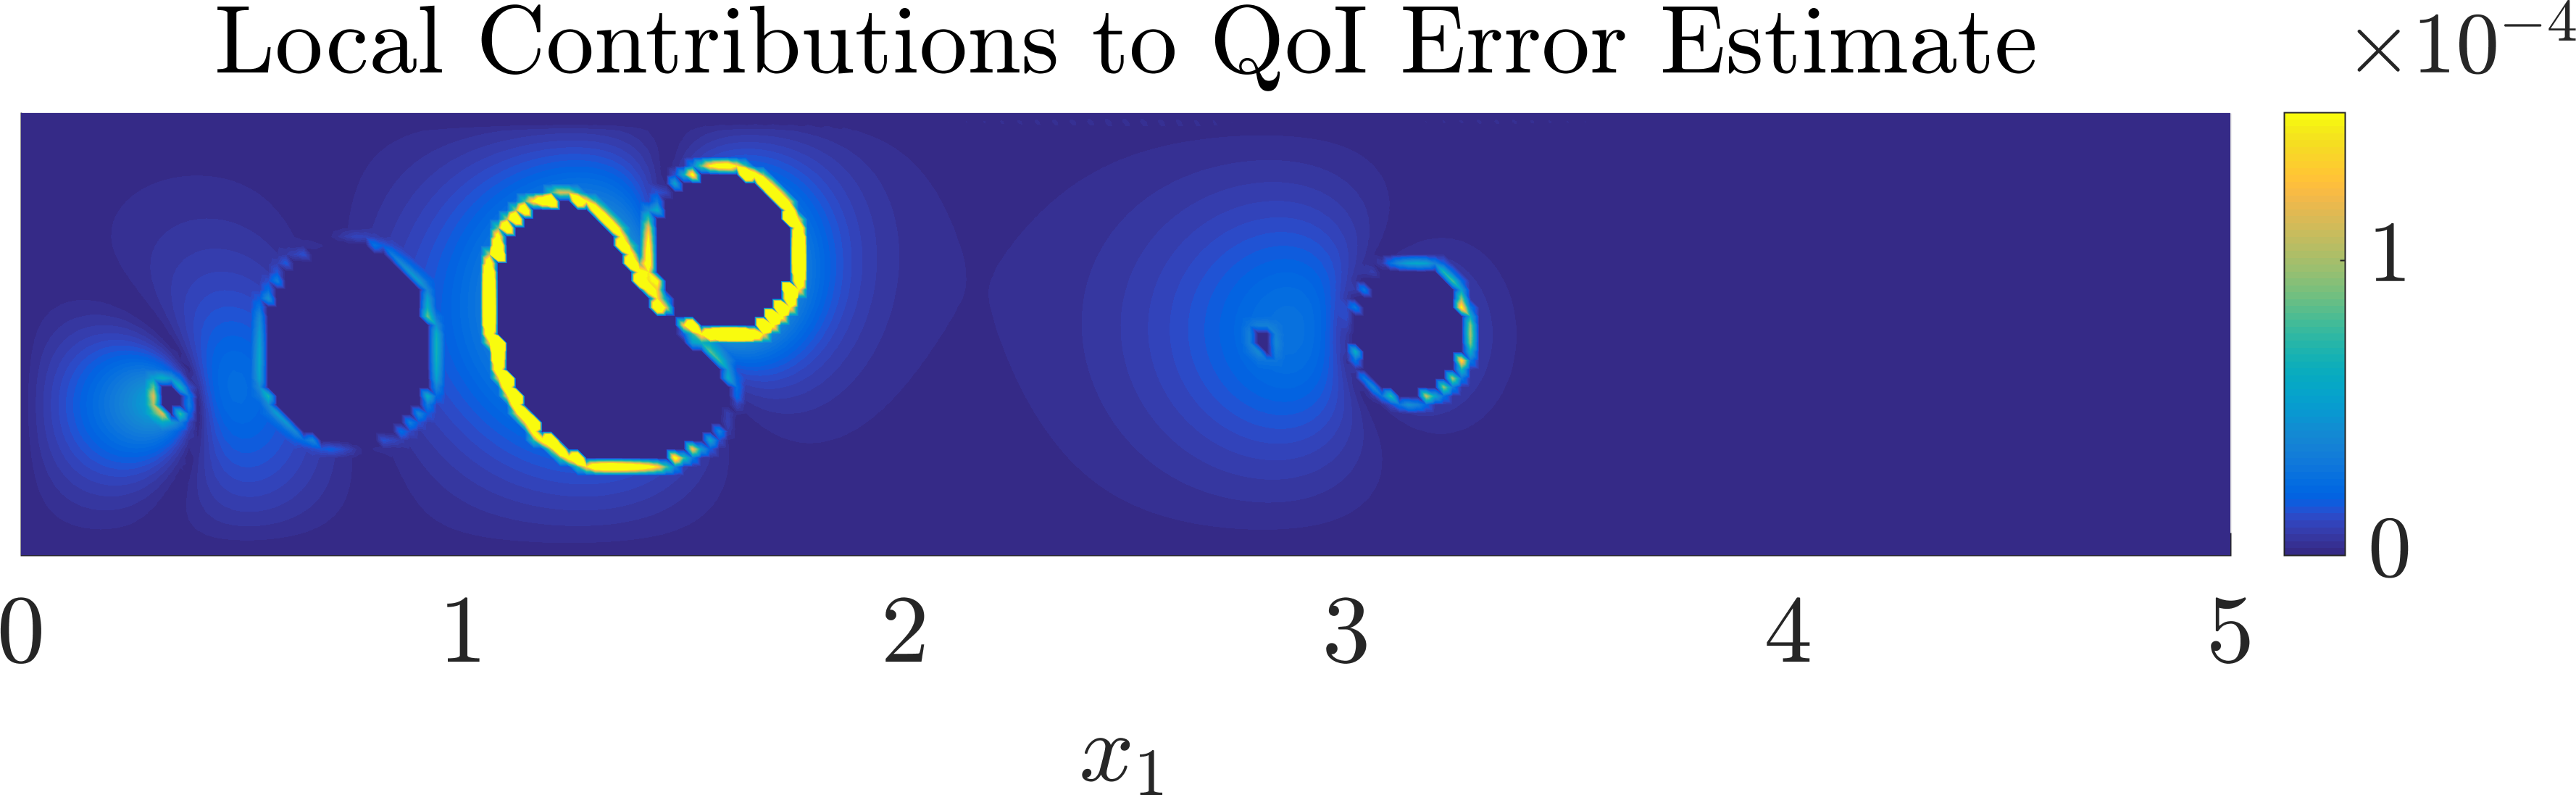
\includegraphics[width=0.49\textwidth]{svf/err_breakdown_MF01.png}
} \\
\subfloat[MF$_2$ ($20\%$ HF)]{
  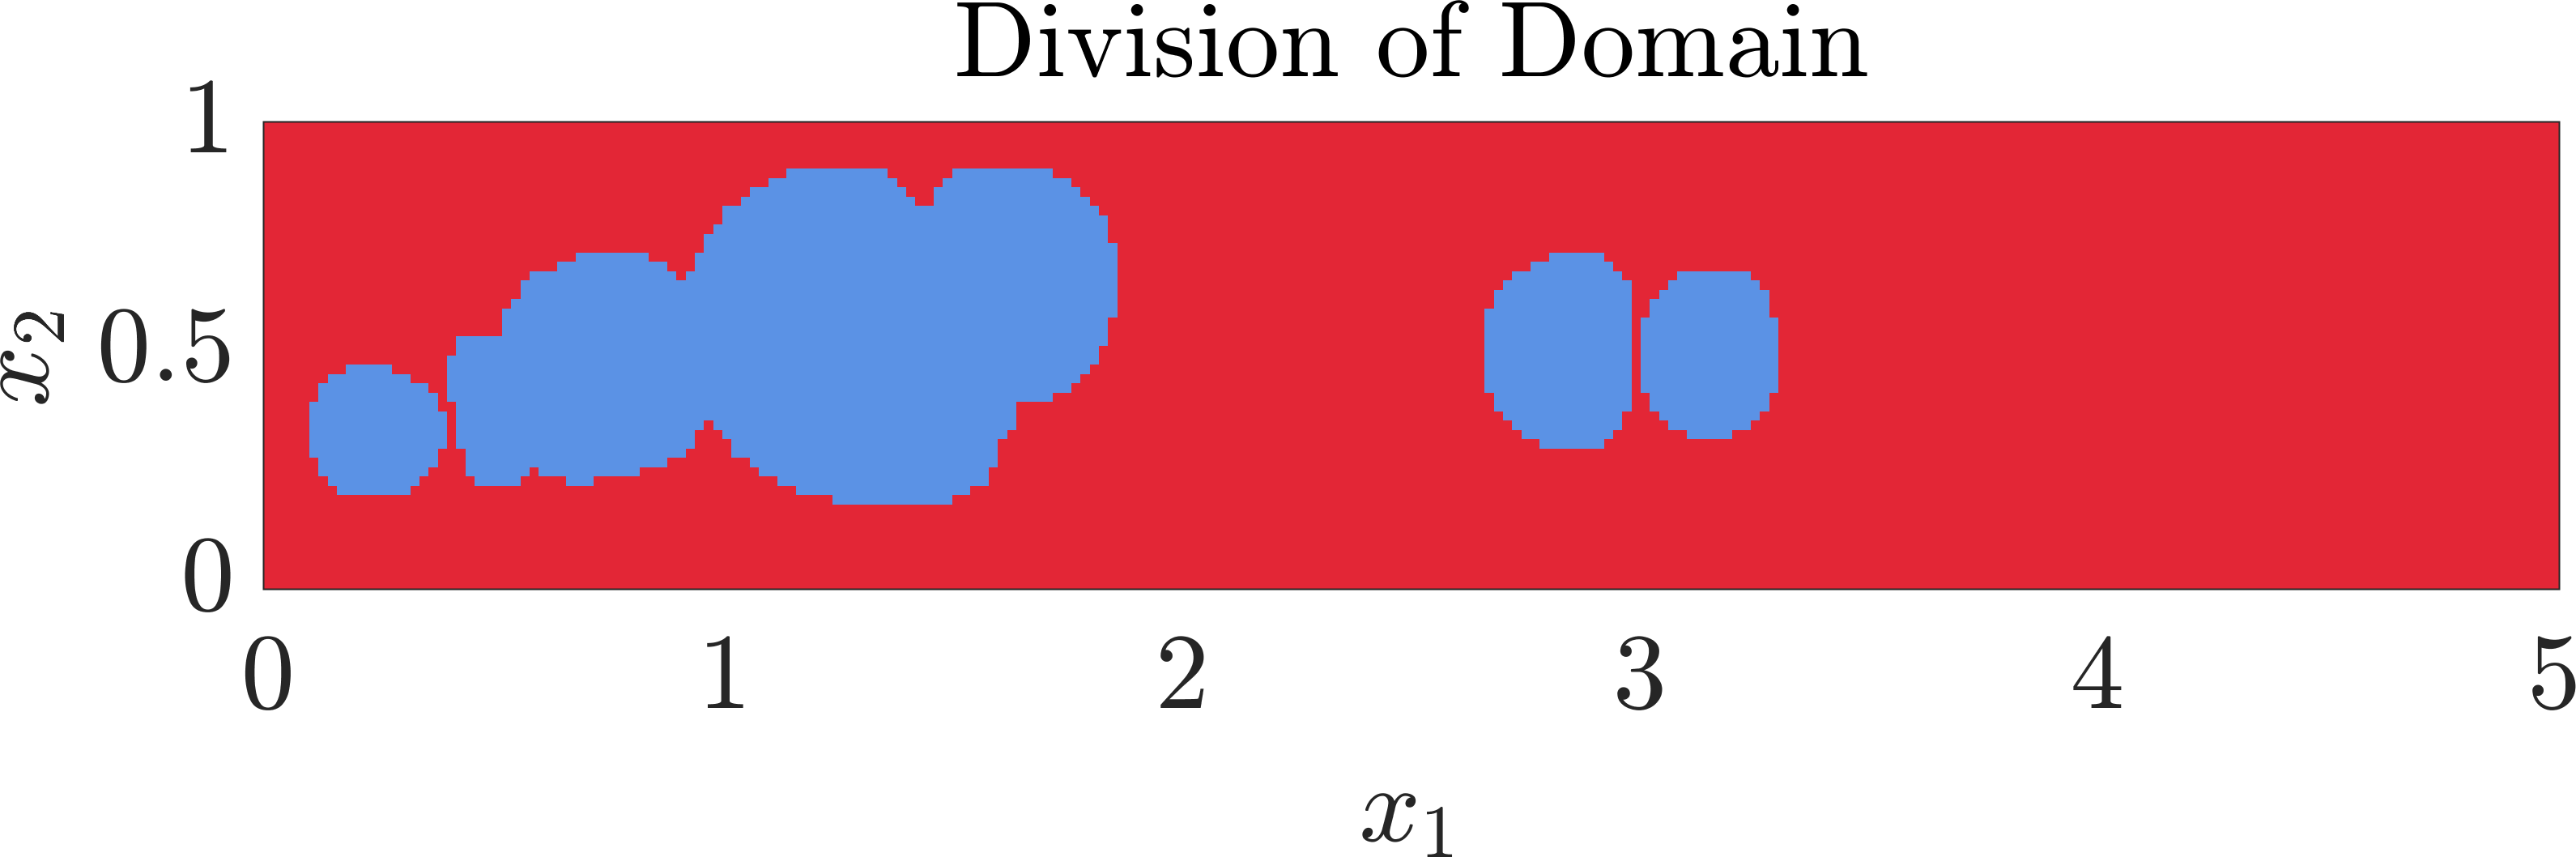
\includegraphics[width=0.46\textwidth]{svf/cd_cdr_MF02_divvy.png}
  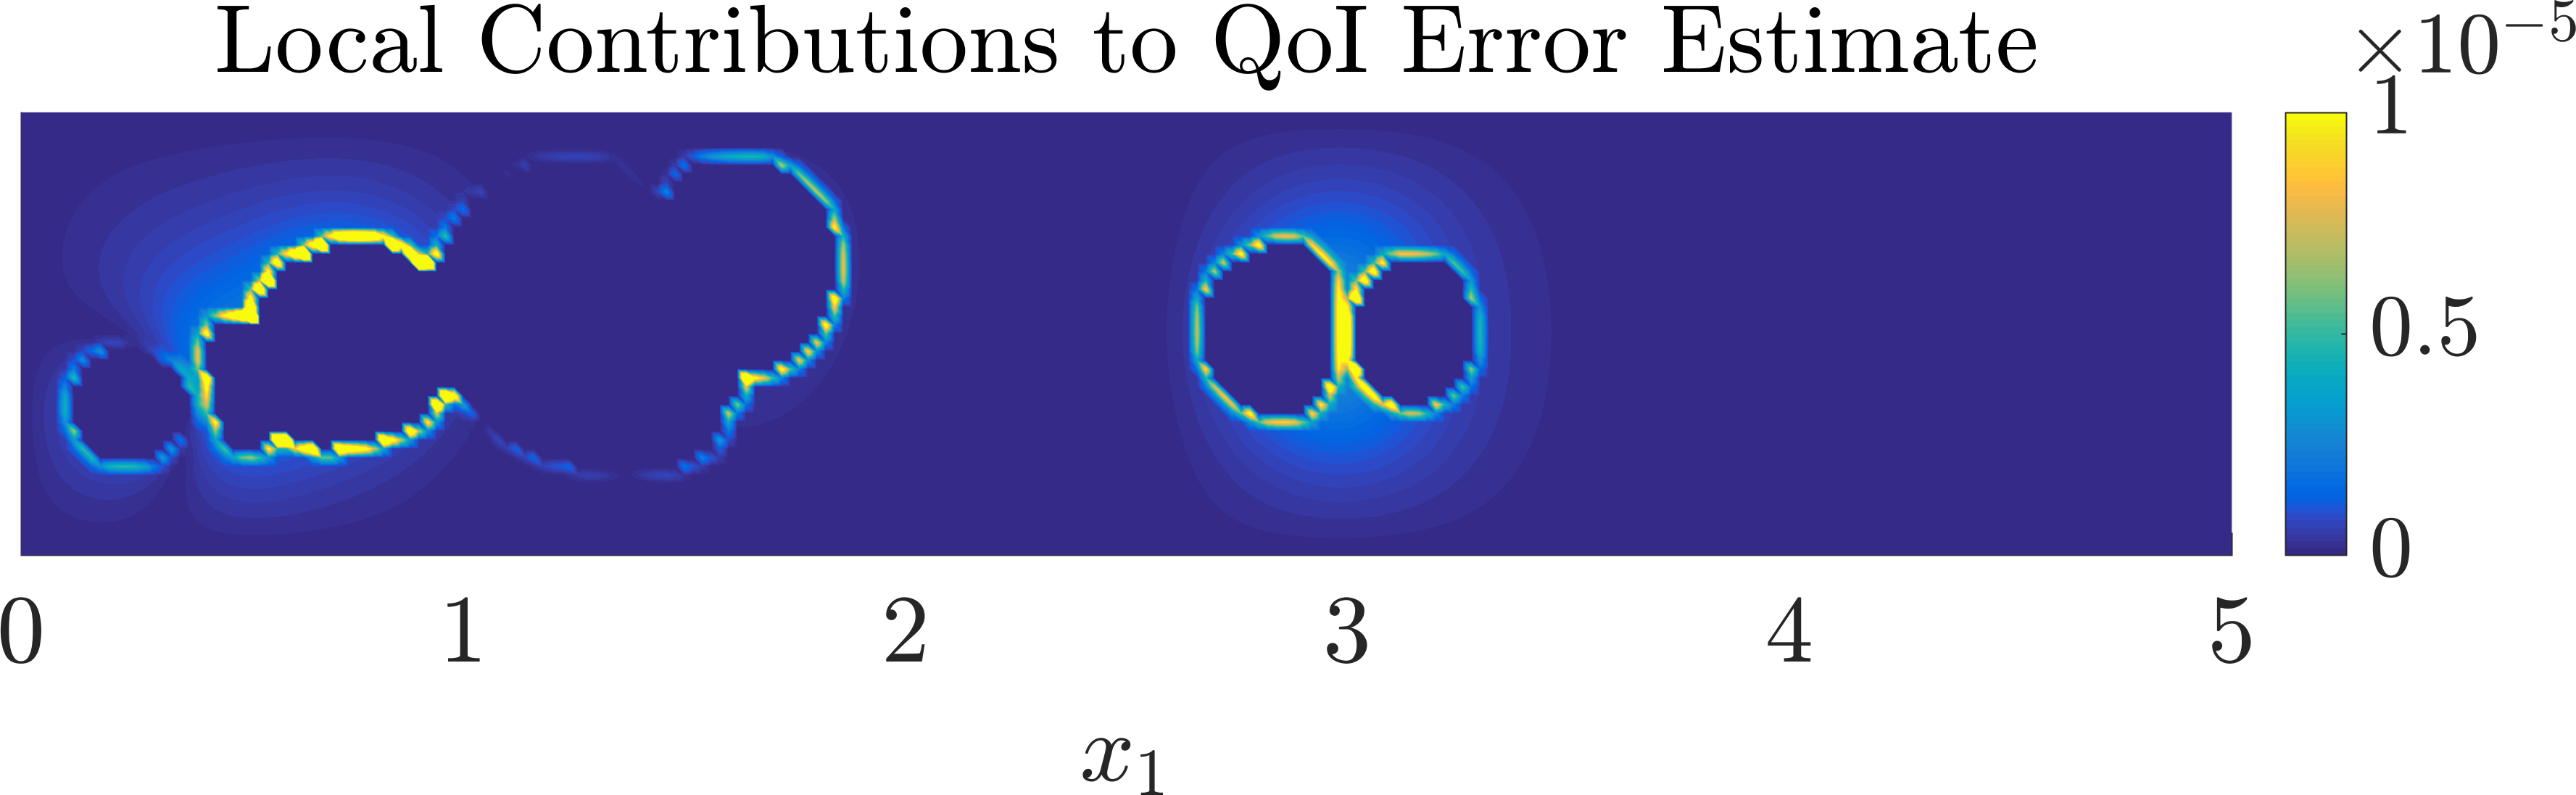
\includegraphics[width=0.49\textwidth]{svf/err_breakdown_MF02.png}
} \\
%\begin{subfigure}[b]{\textwidth}
%	\centering
%	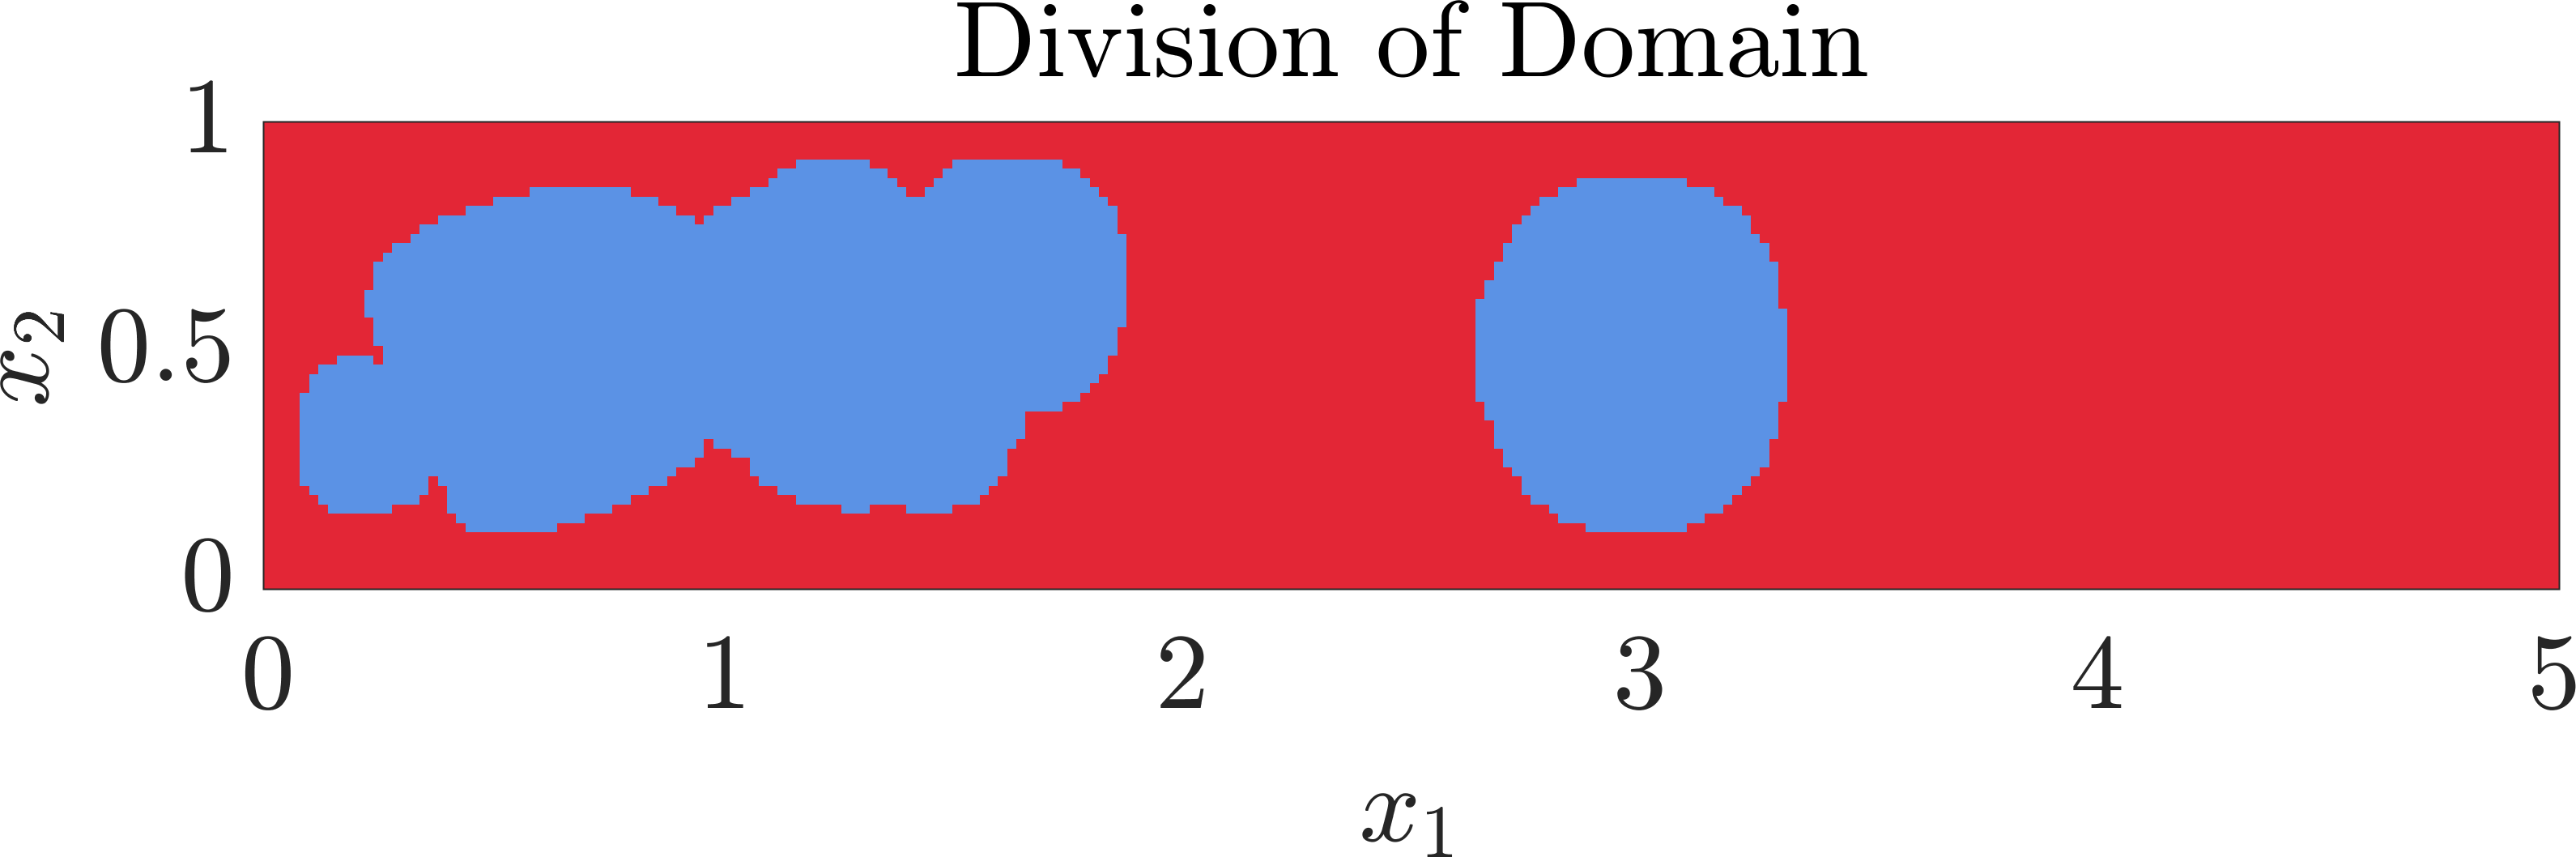
\includegraphics[width=0.48\textwidth]{svf/cd_cdr_MF03_divvy.png}
%  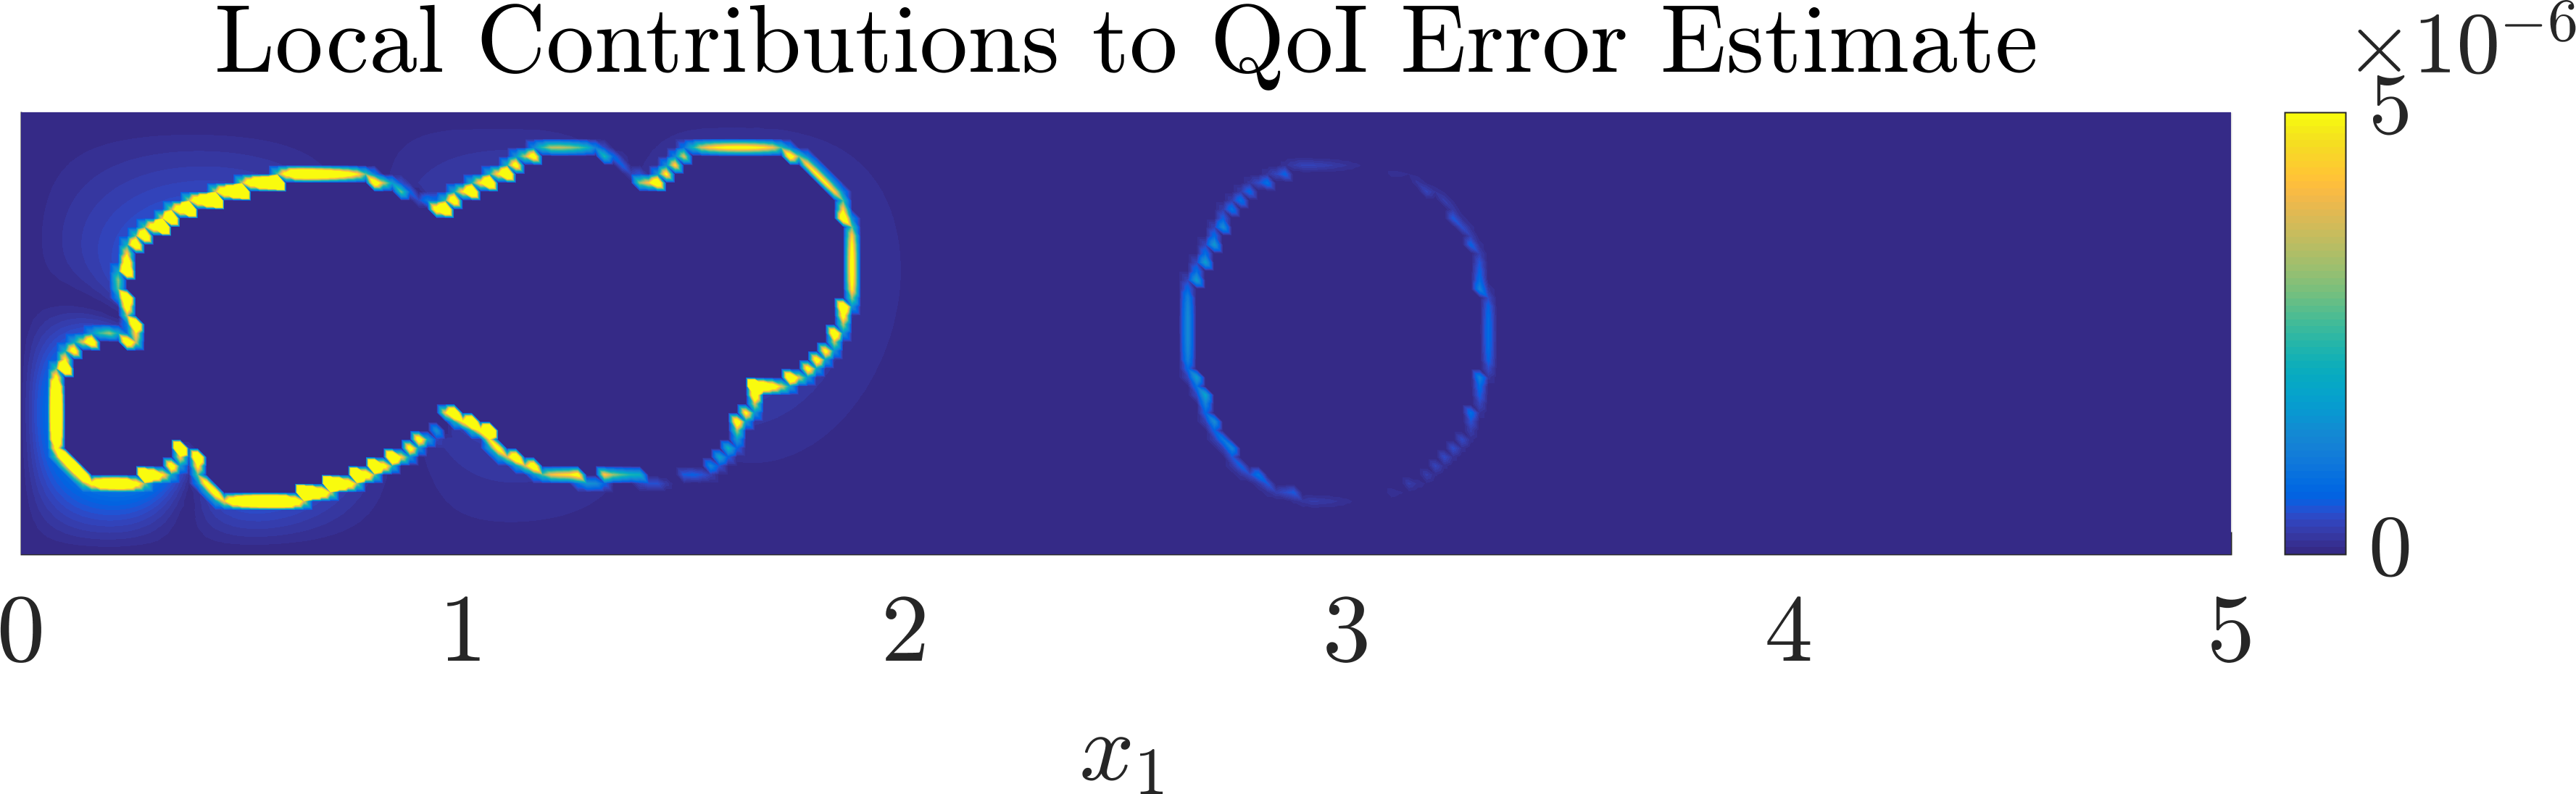
\includegraphics[width=0.51\textwidth]{svf/err_breakdown_MF03.png}
%  \vspace{-0.7\baselineskip}
%  \caption{MF$_3$ ($30\%$ HF)}
%  \vspace{0.8\baselineskip}
%\end{subfigure}
%\begin{subfigure}[b]{\textwidth}
%	\centering
%	
\includegraphics[width=0.48\textwidth]{svf/cd_cdr_MF04_divvy.png}
%  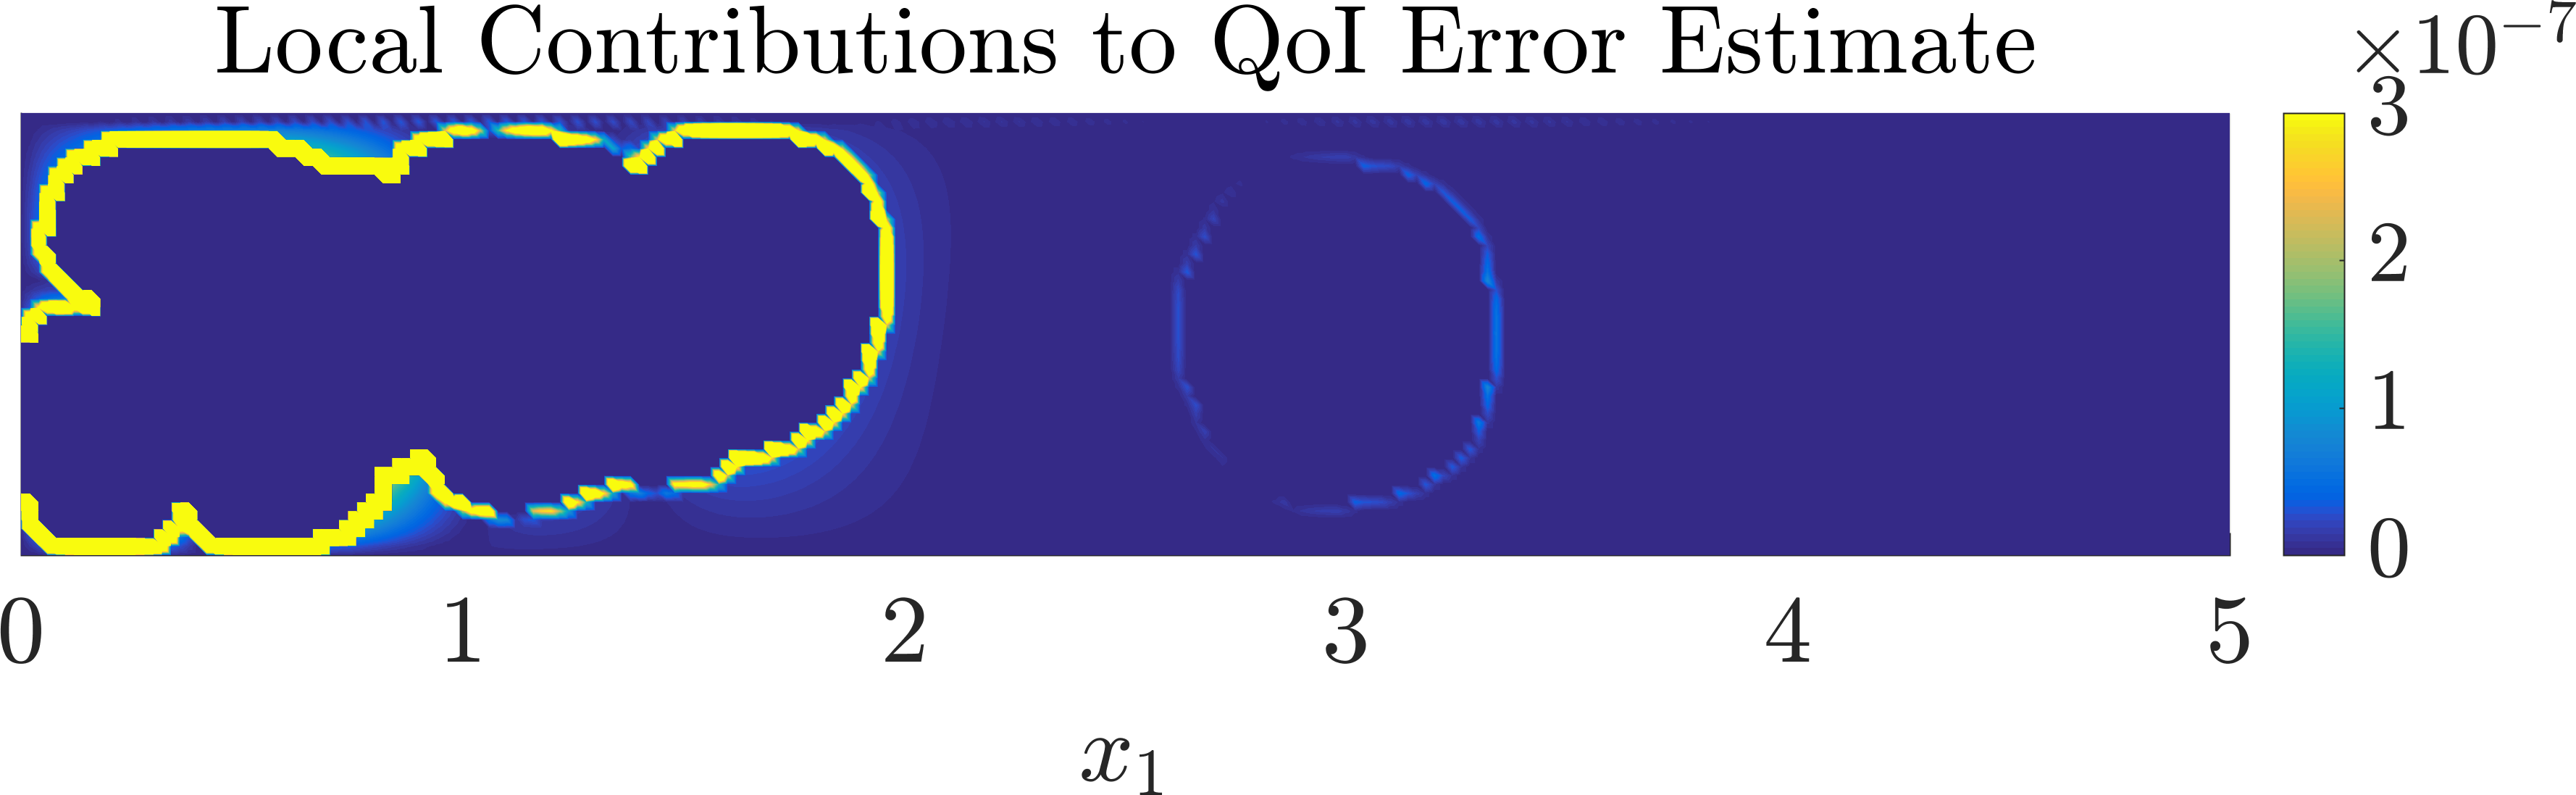
\includegraphics[width=0.51\textwidth]{svf/err_breakdown_MF04.png}
%  \vspace{-0.7\baselineskip}
%  \caption{MF$_4$ ($40\%$ HF)}
%  \vspace{0.8\baselineskip}
%\end{subfigure}
%\begin{subfigure}[b]{\textwidth}
%	\centering
%	
\includegraphics[width=0.48\textwidth]{svf/cd_cdr_MF05_divvy.png}
%  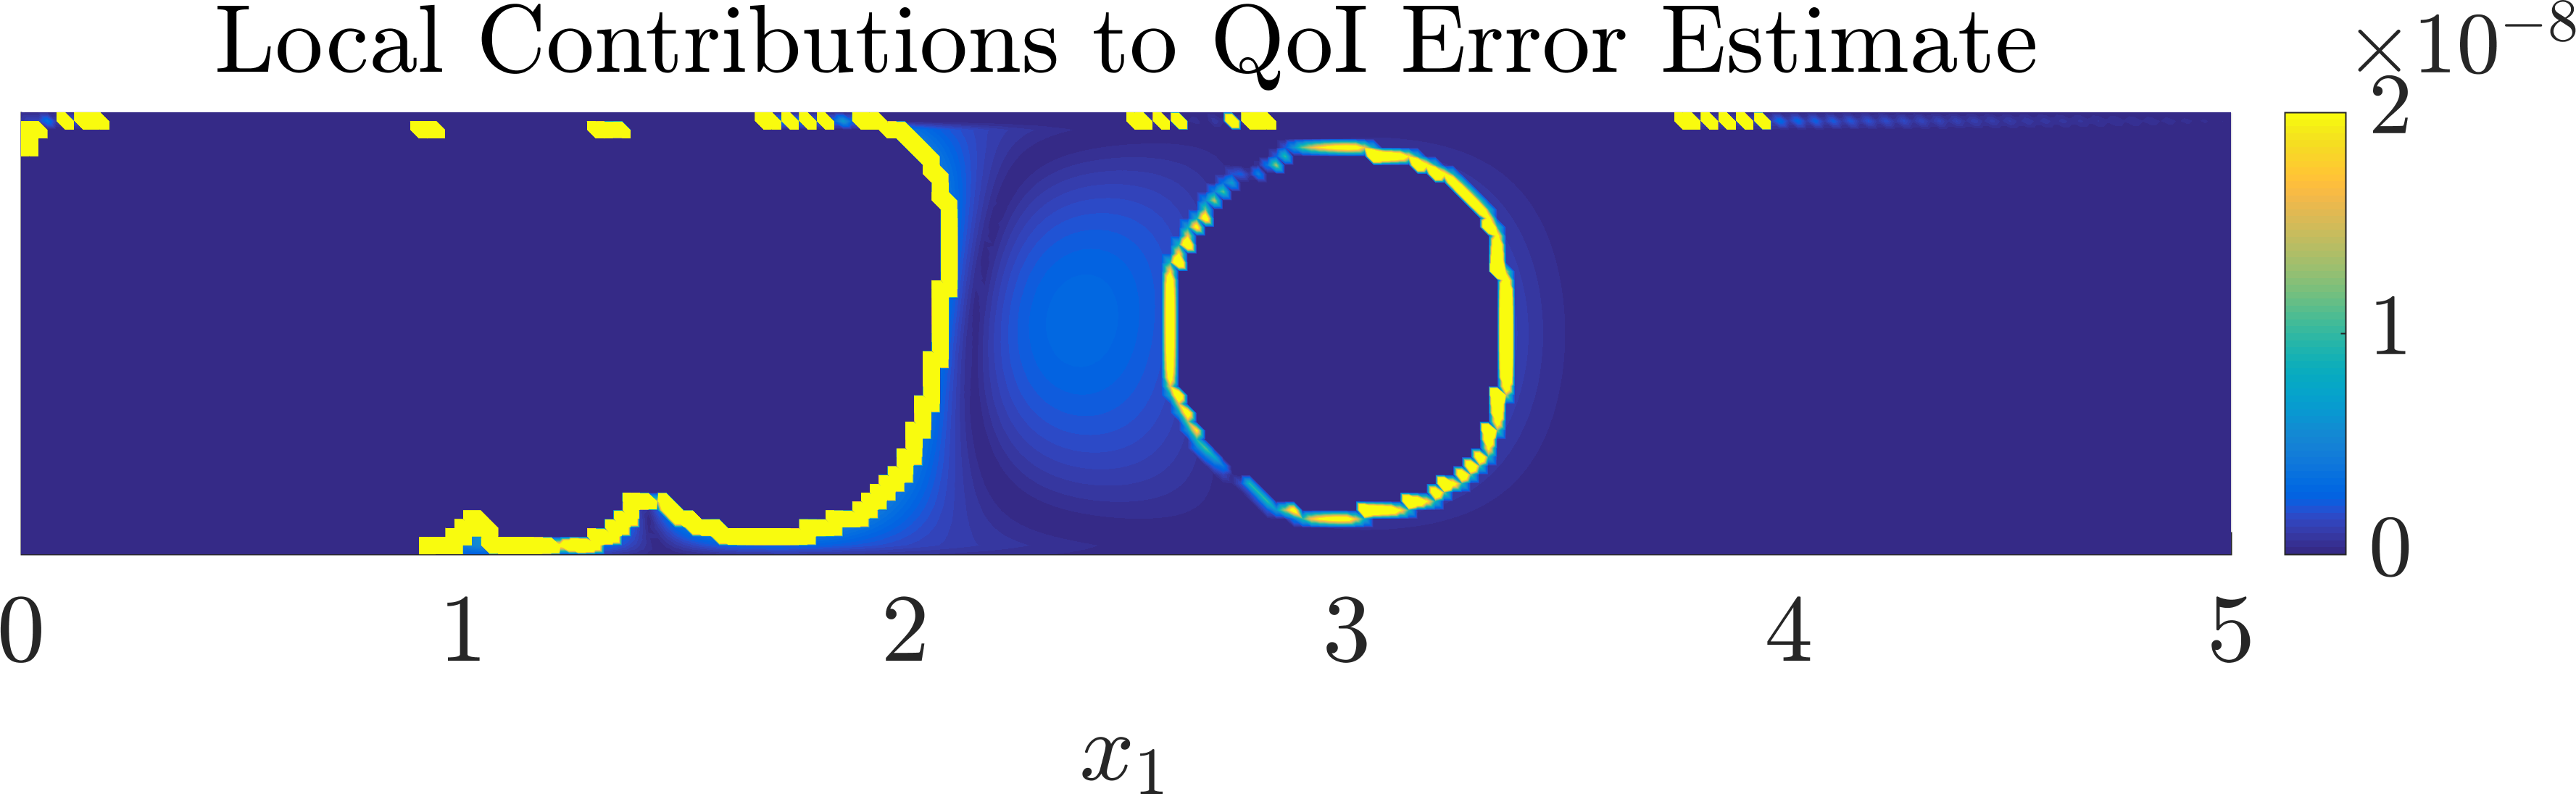
\includegraphics[width=0.51\textwidth]{svf/err_breakdown_MF05.png}
%  \vspace{-0.7\baselineskip}
%  \caption{MF$_5$ ($50\%$ HF)}
%  \vspace{0.8\baselineskip}
%\end{subfigure}
\subfloat[MF$_6$ ($60\%$ HF)]{
	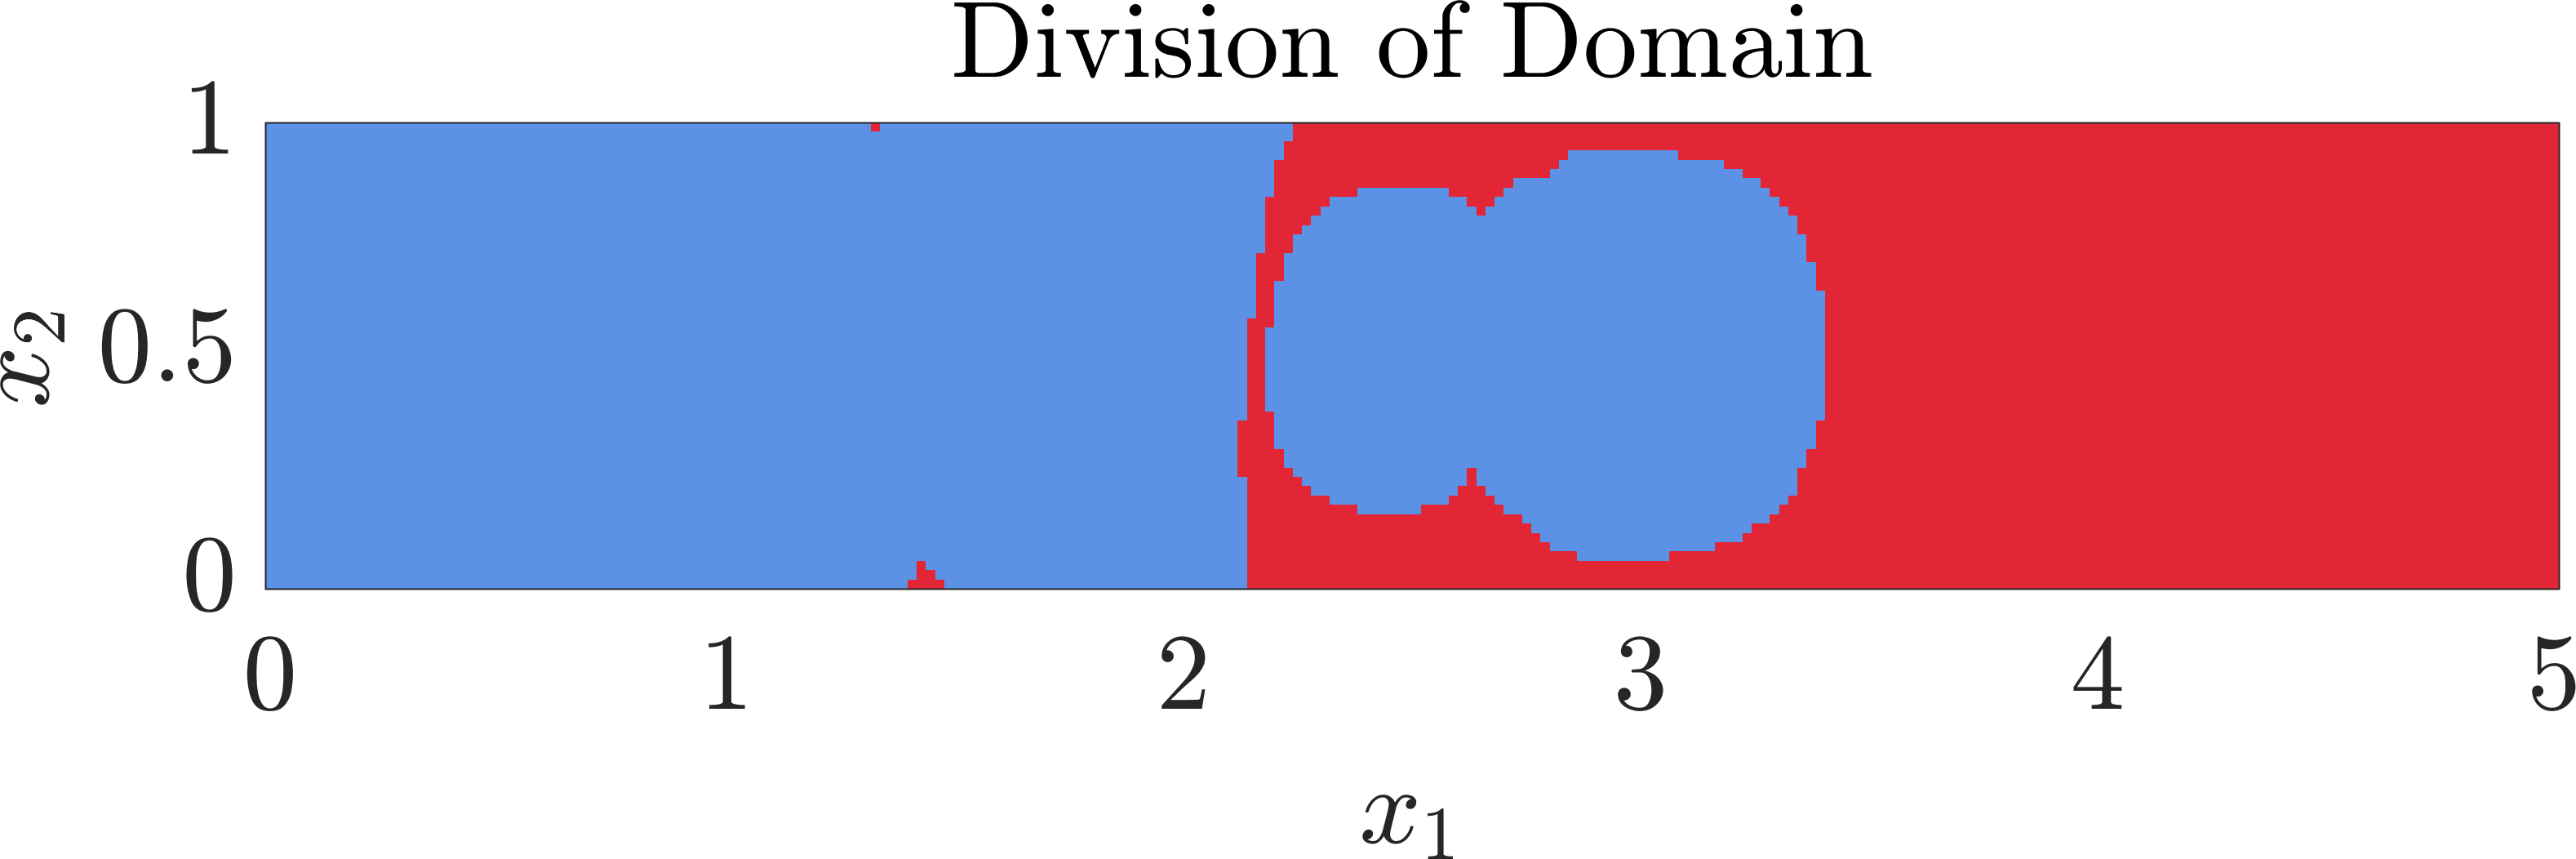
\includegraphics[width=0.46\textwidth]{svf/cd_cdr_MF06_divvy.png}
  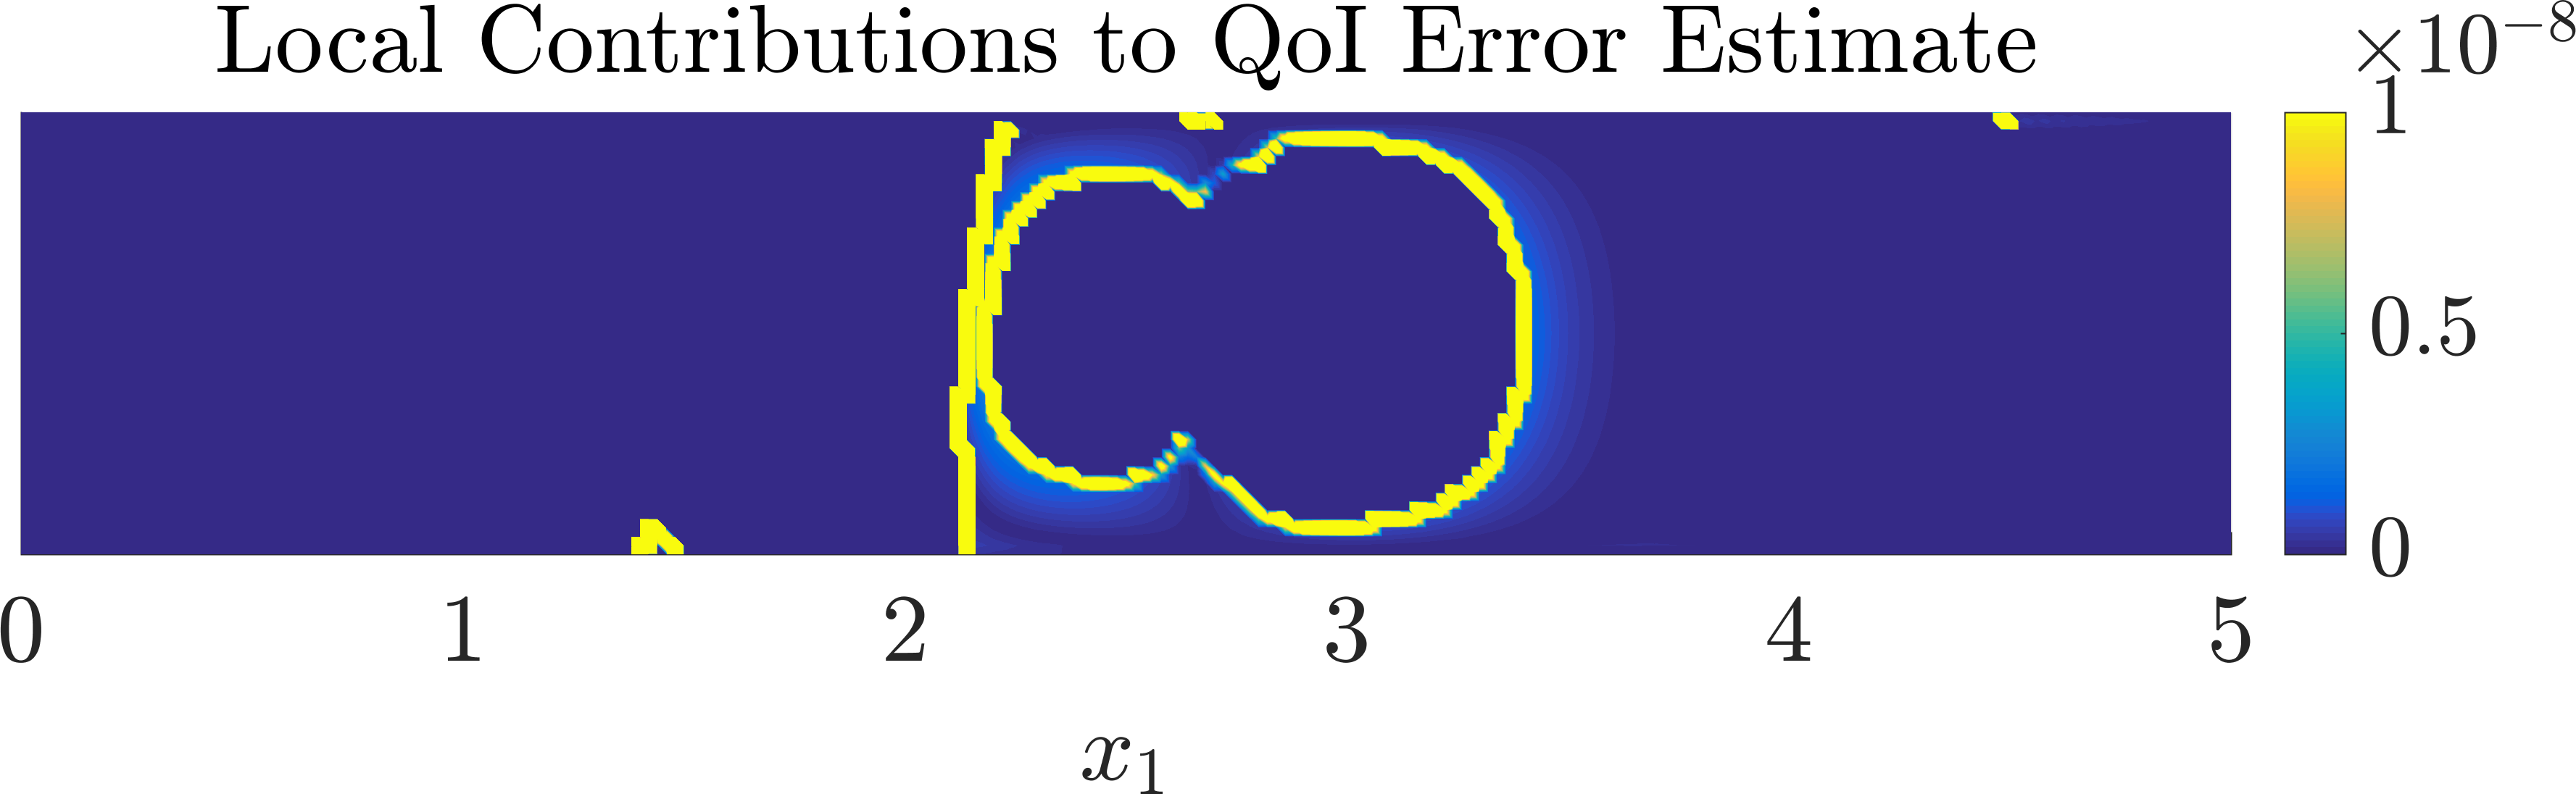
\includegraphics[width=0.49\textwidth]{svf/err_breakdown_MF06.png}
}
\caption{Local error contributions (right) and domain division (left; low-fidelity constant-parameter model used in red portion, high-fidelity field-parameter model used in blue portion) for mixed-fidelity models. The (weighted) residual, and thus the local error contribution, tends to spike sharply at the interface between the low- and high-fidelity regions; the color range is truncated to make the error distribution visible elsewhere in the domain.}
\label{fig:svfRef}
\end{figure}
%
Comparing to \cref{fig:baseRef}, we see that in this case the local error contribution is not as greatly concentrated around the QoI region and the nearest data point; here, all three data points and the QoI region have associated regions of sufficiently similar high local error that all are refined in the first iteration. This reflects the global nature of the differences between the low- and high-fidelity models; the parameter field in all the low-fidelity regions is constant and equal. 

The corresponding true and estimated absolute errors in the QoI are shown in \cref{fig:svfErr}.
%
\begin{figure}[htbp]
\centering
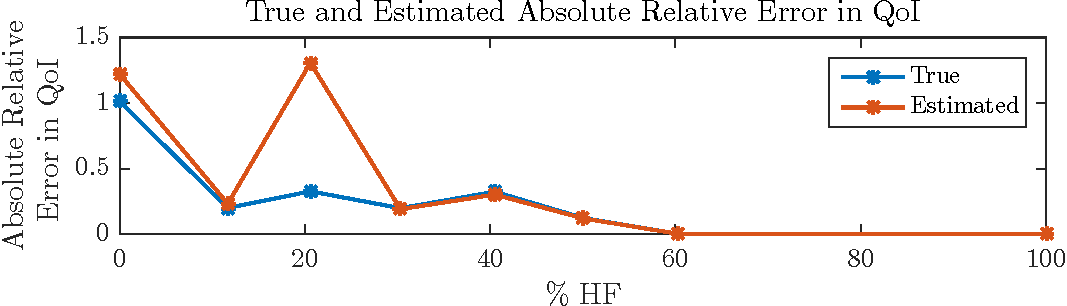
\includegraphics[width=0.8\textwidth]{svf/err_est.pdf}
\caption{True and estimated absolute relative error in QoI, plotted as a function of the percentage area of the domain in which the high-fidelity field-parameter model is used.}
\label{fig:svfErr}
\end{figure}
%
In this case, we see that we must use the high-fidelity model in most of the domain in order to get an accurate QoI. The adaptive algorithm requires us to use the field representation of the high-fidelity model in much of the left half of the domain; this reflects the topology of the inferred parameter field in the high-fidelity inverse problem, which is only relatively constant towards the right portion of the domain. We also see that in this case, compared to the example in \cref{sec:cdvcdrBaseRef}, increasing the proportion of the domain in which the high-fidelity model is used does not monotonically decrease the error in the QoI. 

%------------------------------------------------------------------------------------------------------------------------%
\subsection{Combining Meshes and Physics in 3D} \label{sec:diffvcdr3D}
%------------------------------------------------------------------------------------------------------------------------%

In the previous examples, although the low- and high-fidelity models are sufficiently different to illustrate the behavior of \cref{alg:refSeries}, they are both simple enough and similar enough that using \cref{alg:refSeries} saves little, if any, time. In this section, we consider a more realistic pair of models which differ in both the physics included and the mesh resolution, and demonstrate computational savings. In \cref{sec:setup3D_diffmesh} we describe the setup of the models and their inverse problems, and in \cref{sec:ref3D_diffmesh} we describe the results of applying \cref{alg:refSeries} to this pair of models.

%------------------------------------------------------------%
\subsubsection{Problem Setup} \label{sec:setup3D_diffmesh}
%------------------------------------------------------------%

The two models share a box domain $\Omega(x_1,x_2,x_3)$ which is $2300$m, $1650$m, and $100$m long in the $x_1$, $x_2$, and $x_3$ directions, respectively. We will refer to the positive and negative directions in $x_1$ as ``east" and ``west", respectively. The high-fidelity model is a single-species convection-diffusion-reaction equation with a nonlinear reaction term, described by
%
\begin{subequations}
\label{eq:cdvcdrHF3D}
\begin{align}
\nabla\cdot(n\vec{V}u - nD\nabla u) + k_ru^2 = f(q) \quad &\text{in } \Omega, \label{eq:HFeq3D}\\
u = 0 \quad &\text{on } \partial \Omega_{west}, \\
\frac{\partial u}{\partial n} = 0 \quad &\text{on }\partial\Omega_{east}, \\
\hat{n}\cdot(n\vec{V}u - nD\nabla u) = 0 \quad &\text{on }\partial\Omega\backslash(\partial\Omega_{east}\cup\partial\Omega_{west}),
\end{align} 
\end{subequations}
%
where the state $u$ is the mass-fraction (in parts-per-billion) of some contaminant species and $f(q)$ is a source/sink field. The velocity field is a constant $\vec{V}=(2.1,0,0)$ m/day. Given this velocity field and letting the molecular diffusion be negligble, we follow \cite{Vestedetal93} to express the (diagonal) dispersion tensor $D$ as $D_{11}=\alpha_{LH}V_1$, $D_{22}=\alpha_{TH}V_1$, and $D_{33}=\alpha_{TV}V_1$, where $\alpha_{LH}=100$m, $\alpha_{TH}=40$m, and $\alpha_{TV}=4$m are the longitudinal horizontal, transverse horizontal, and transverse vertical dispersivities, respectively; the dispersivity values were drawn from within the range of observed values in various porous media \cite{Davis86}. We have porosity $n=0.1$. The reaction coefficient is $k_r=4.2\cdot10^{-4}$ 1/day, chosen from within the wide range of reaction-rate coefficients for second-order reactions. Although the reaction term $k_ru^2$ does not correspond to any particular reaction of any particular species, we note that, in addition to second-order elementary reactions, a quadratic reaction term can appear in models of dissolution/precipitation processes in porous media \cite{Aha97} and biochemical degredation of petroleum hydrocarbons in soils \cite{Jack94}.

The low-fidelity model,
%
\begin{equation}
\nabla\cdot(- nk_d\nabla u) = f(q) \quad \text{in } \Omega, \label{eq:LFeq3D}
\end{equation}
%
differs in the removal of the reaction and convection terms and the anisotropy of the dispersion tensor; the dispersion tensor $D$ is replaced with a scalar $k_d=D_{11}$. The boundary conditions remain unchanged. As in the previous examples in \cref{sec:cdvcdr}, the mixed-fidelity models are formed by dividing the domain into complementary subdomains $\Omega_{HF}$ and $\Omega_{LF}$, where \cref{eq:HFeq3D,eq:LFeq3D} are solved, respectively. The QoI we wish to calculate is again an integral of the state over a region $\Omega_I$. 

The unknown parameters we wish to infer correspond to the source term $f(q)=q$; we impose $f(q)=q=0$ on the boundary $\partial\Omega$. Observations at 18 points in the domain are artificially generated by running the high-fidelity model on a finer mesh. The locations of the observations as well as the QoI region $\Omega_I$ are shown in \cref{fig:setup3D}. We use a regularization term $\frac{\beta}{2}\int_\Omega \|\nabla f(q)\|_2^2\:\textrm{d}V$.
%
\begin{figure}[htbp]
\centering
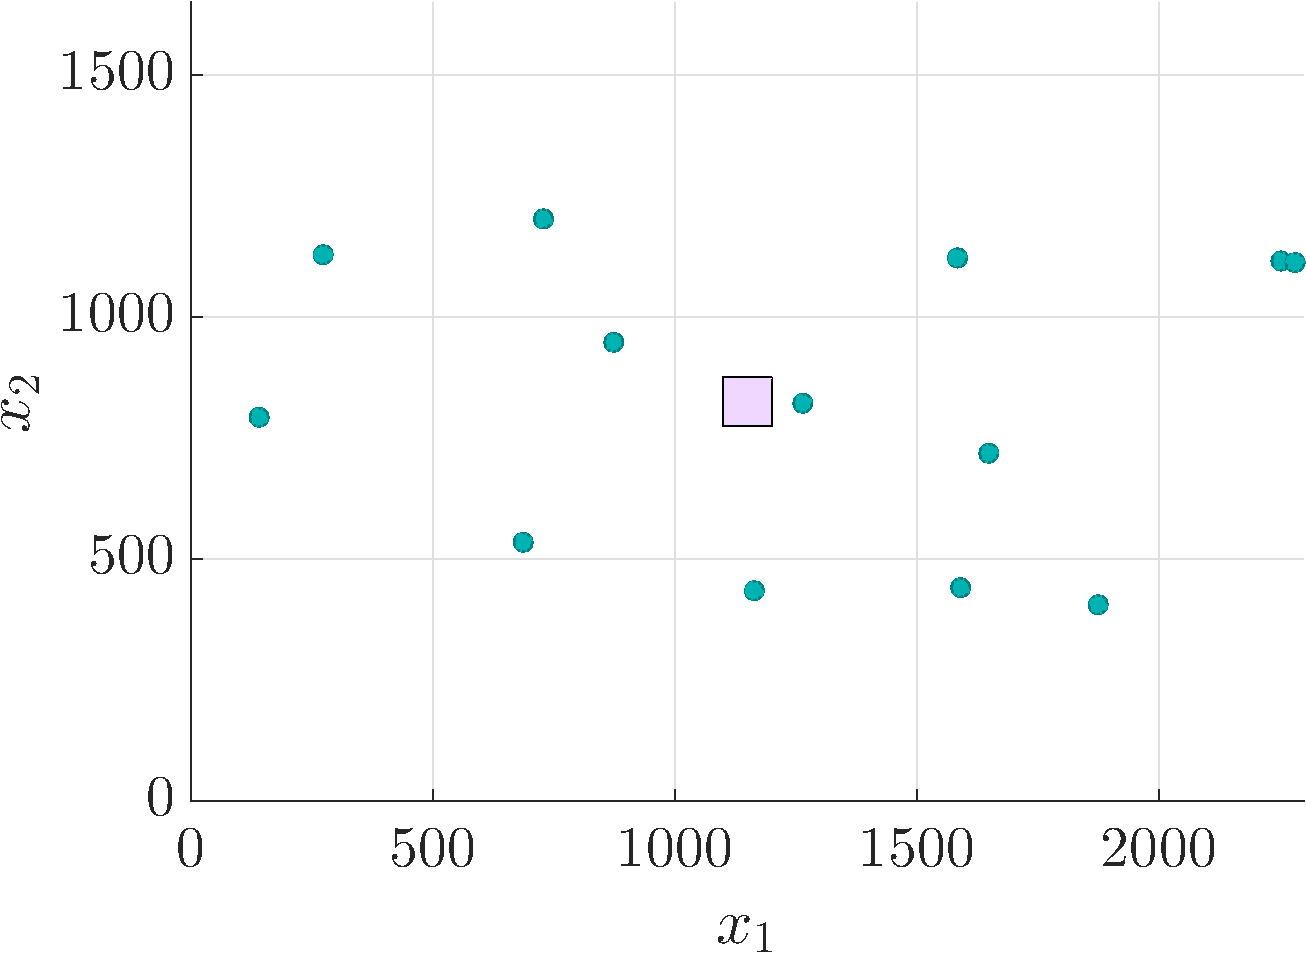
\includegraphics[width=0.4\textwidth]{series3D/setup_aerial_nolegend.pdf} \hfill
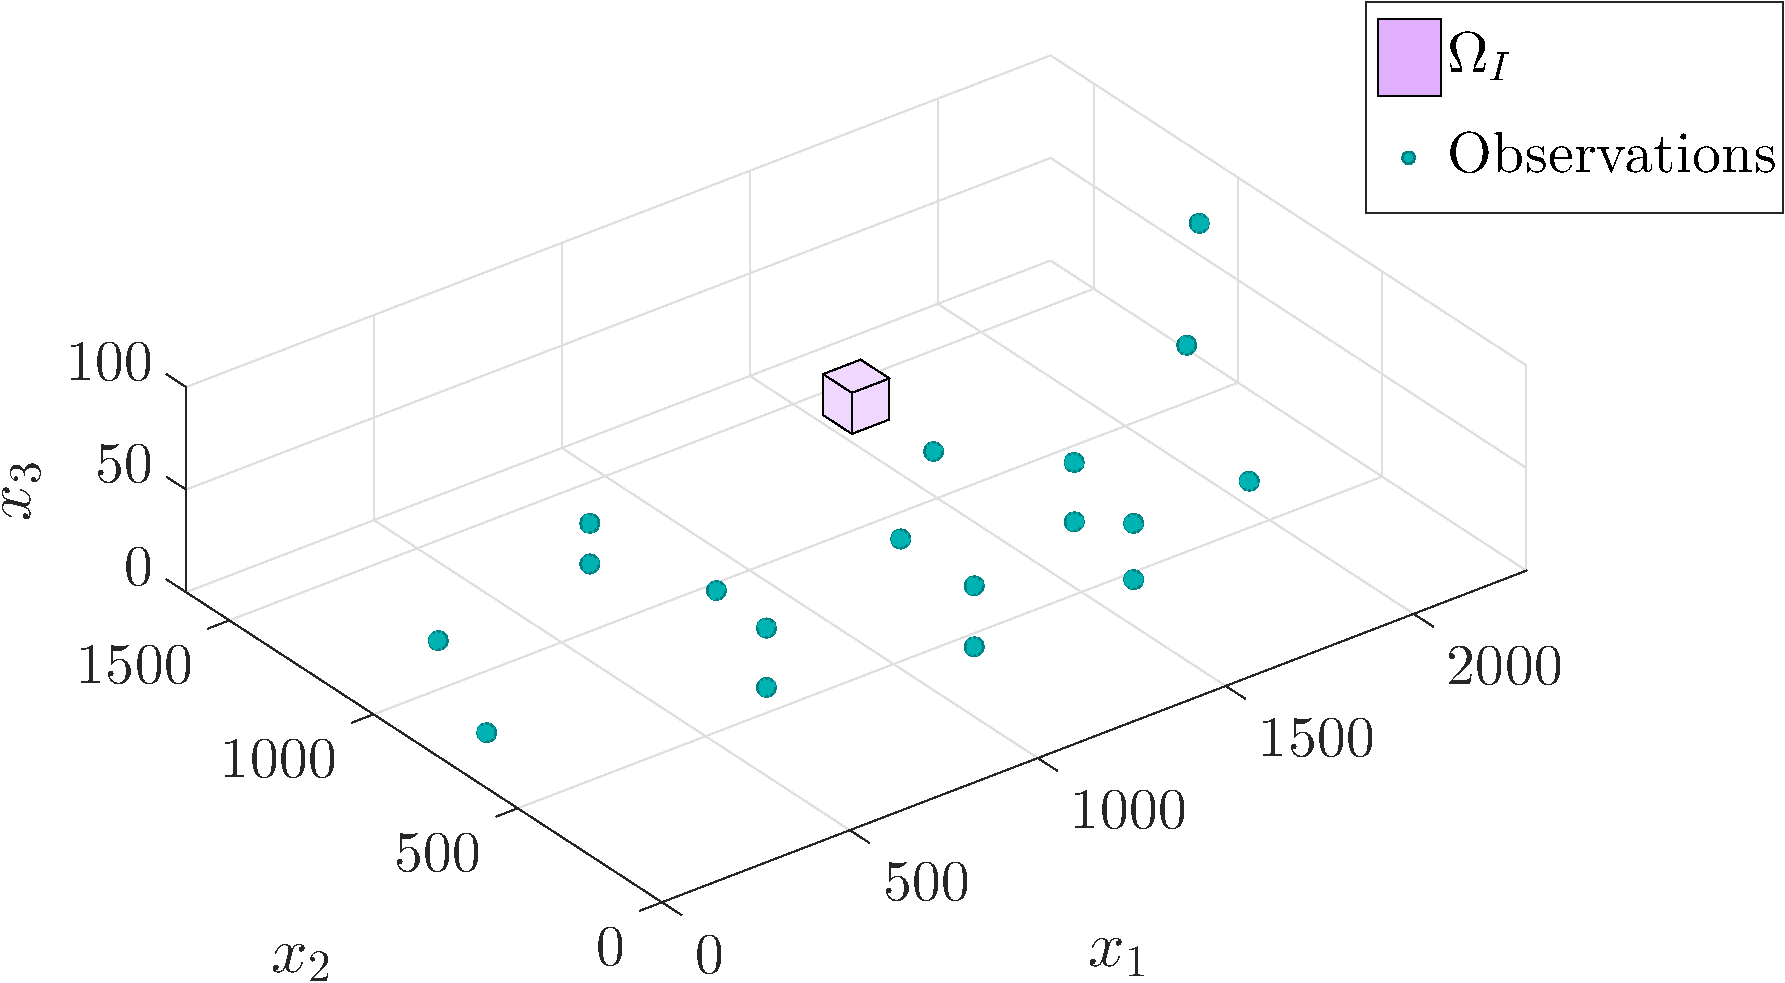
\includegraphics[width=0.55\textwidth]{series3D/setup_3view.pdf} \\ 
\vspace{\baselineskip}
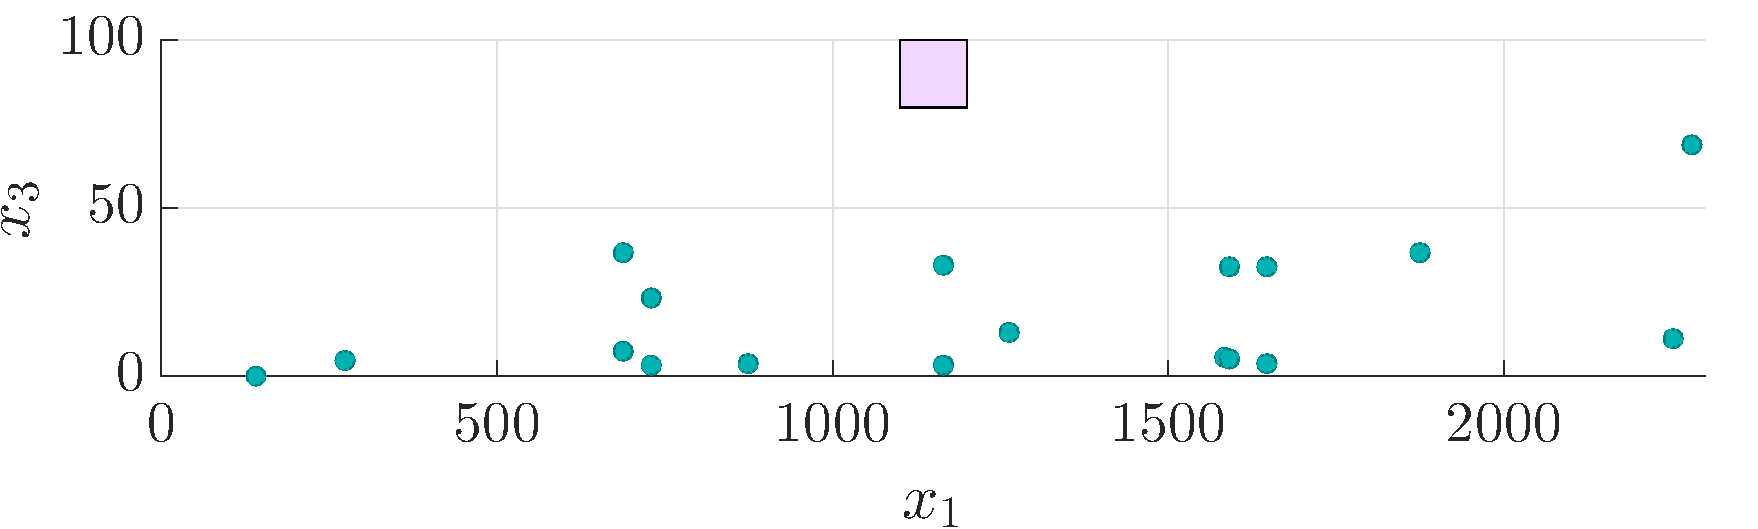
\includegraphics[width=0.6\textwidth]{series3D/setup_side_view.pdf}
\caption{Three views of the locations of the observations and the QoI region.}
\label{fig:setup3D}
\end{figure}
%

We continue to use the FEM with a continuous Galerkin formulation and Lagrange elements. The lack of a convection term allows the low-fidelity model to be solved on a coarser mesh. For the high-fidelity model, the domain is descretized by 32, 64, and 32 elements along the $x_1$, $x_2$, and $x_3$ directions, respectively; for the low-fidelity model, the domain is descretized by 16, 32, and 16 elements along the $x_1$, $x_2$, and $x_3$ directions, respectively. The cell P\'{e}clet number is less than one and so no stabilization is used.

%------------------------------------------------------------%
\subsubsection{Adaptive Model Refinement Results} \label{sec:ref3D_diffmesh}
%------------------------------------------------------------%

We now present the results of solving the inference problem using \cref{alg:refSeries}, with a relative error tolerance of $0.1\%$. At each iteration, we choose the $2\%$ of the basis functions with the largest error for model refinement; since each linear Lagrange basis function has eight elements in its support, the number of additional elements marked for refinement in each iteration is usually greater. All simulations are run on a single processor; we use the default nonlinear solver in \texttt{libMesh} (Newton's method with Brent line-search), and linear solves are performed using PETSC's GMRES solver, preconditioned by incomplete factorization. 

\Cref{tab:ref3D_diffmesh} shows the error at the end of each adaptive iteration. Each iteration of the adaptive algorithm uses the solution of the previous iteration as its initial guess. The number of degrees of freedom of each of the primary (and, if applicable, auxiliary) variables at each iteration is also given; the supplementary adjoint is solved on the high-fidelity mesh and thus each of its variables has the same number of degrees of freedom as each of the primary variables in the high-fidelity inverse problem. The high-fidelity inverse problem does not converge when the low-fidelity solution is used as an initial guess. Instead, we solve the inverse problem for an intermediate model 
%
\begin{equation}
\nabla\cdot(n\vec{V}u - nD\nabla u) + k_ru^2 = f(q)
\end{equation}
%
and use the solution as an initial guess for the high-fidelity problem; equivalently, we use two steps of natural continuation on the reaction parameter: $k_r=0$, then $k_r=4.2\cdot10^{-4}$. 
%
\begin{table}[htbp]
\caption{Runtime and relative errors of adaptive algorithm iterations given relative error tolerance of $0.1\%$; relative errors are given with respect to the true high-fidelity QoI.}
\label{tab:ref3D_diffmesh}
\centering
\begin{tabular}{|c|c|c|c|c|c|c|c|c|}
\hline
\multirow{2}{*}{Case} & \multirow{2}{*}{$\%$HF} & \multirow{2}{*}{DOFs} & \multirow{2}{*}{QoI} & Error & Error & $\%$ Relative \\ 
& & & & (Estimated) & (Actual) & Error (Actual)  \\ \hline
LF   & 0    & 9537  & 168710 & -16463 & -85663 & -103    \\
MF01 & 5.2  & 13417 & 167366 & -7207  & -84319 & -102    \\
MF02 & 11.4 & 17895 & 89777  & -6208  & -6730  & -8.10   \\
MF03 & 16.3 & 21001 & 85880  & -2473  & -2833  & -3.41   \\
MF04 & 22.0 & 24528 & 83902  & -711   & -855   & -1.03   \\
MF05 & 27.7 & 27984 & 83119  & 32     & -72    & -0.087  \\
HF   & 100  & 70785 & 83047  & --     & --     & --    \\ \hline
\end{tabular}
\end{table}
%

We notice that, compared to the results in \cref{fig:baseErr}, the error estimates for the low-fidelity and first mixed-fidelity models are very far from the true errors. This can be attributed to the linearization about $\Psi_{LF}$ and $\Psi_{MF_{1}}$ instead of $\Psi_{HF}$ in solving the supplementary adjoints; the large differences in the QoI for the LF and MF01 models compared to the high-fidelity QoI indicate that $\Psi_{LF}$ and $\Psi_{MF_{1}}$ are very different from $\Psi_{HF}$. Compared to the pair of models in \cref{sec:cdvcdrSetup}, the low- and high-fidelity models are more disimilar, even though the nonlinear term in the high-fidelity models remain the same. This behavior suggests that one should use more than just the error estimate to decide when to stop the adaptive algorithm; a possible additional criterion could be to require that the predicted high-fidelity QoI $I(q_{MF},u_{MF})+\epsilon_i$ for two consecutive iterations agree to within some tolerance.

The domain divisions for the five adaptive iterations are shown in \cref{fig:divvy3D_diffmesh}. Similarly to the behavior seen in \cref{sec:cdvcdrBaseRef}, the QoI region and the areas around some of the measurement points are first targeted for refinement, with those measurement points furthest downstream of the QoI being the last to be refined around. We also see that the domain is refined completely in the $x_3$ direction first around the QoI region, possibly reflecting the large difference in the high-fidelity dispersion tensor $D$ and the low-fidelity dispersion coefficient in the $x_3$ direction.
%
\begin{figure}[htbp]
\centering
\subfloat[MF$_1$ ($5.2\%$ HF)]{
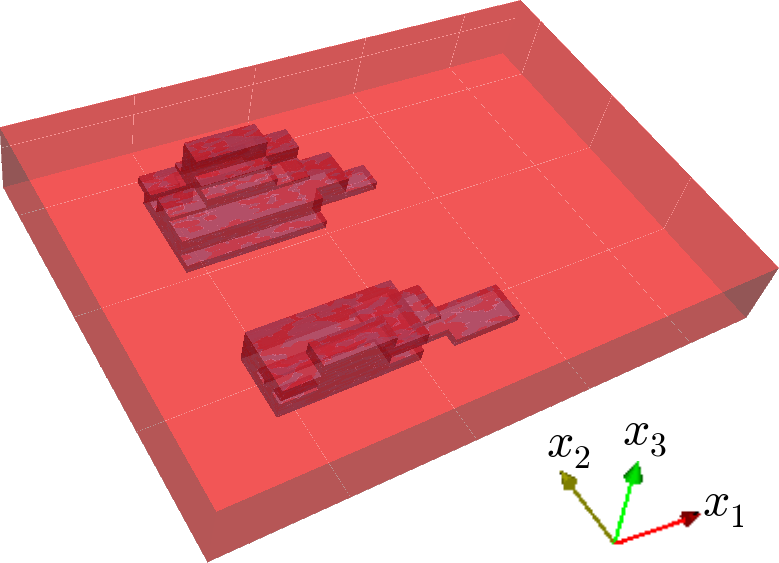
\includegraphics[width=0.31\textwidth]{series3D/run_diff_mesh/divvy1_whitebg_puff.png} 
}
\subfloat[MF$_2$ ($11.4\%$ HF)]{
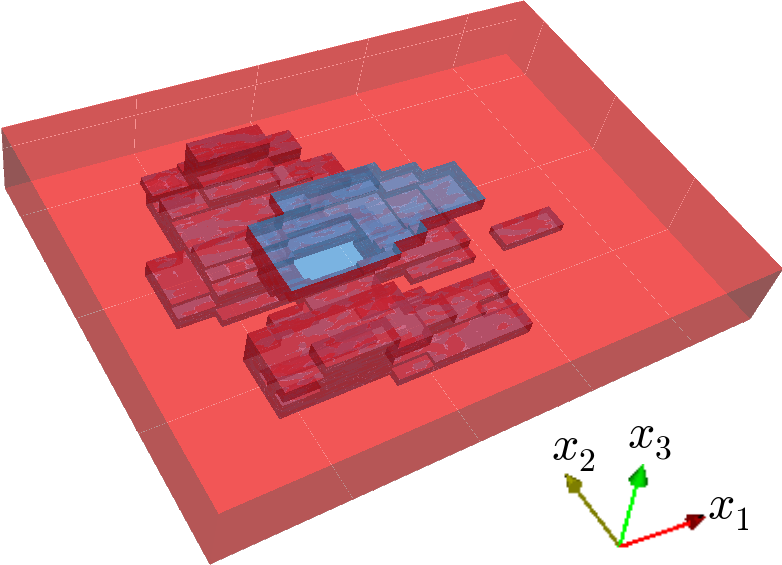
\includegraphics[width=0.31\textwidth]{series3D/run_diff_mesh/divvy2_whitebg_puff.png} 
}
\subfloat[MF$_3$ ($16.3\%$ HF)]{
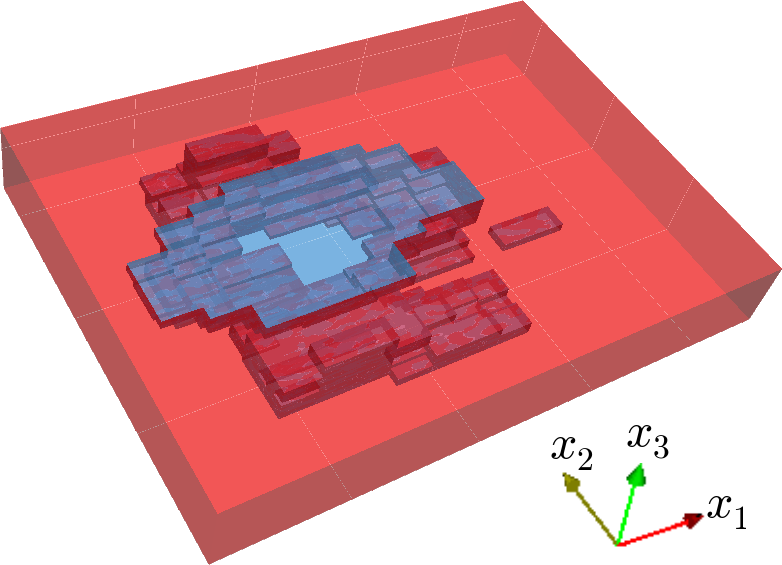
\includegraphics[width=0.31\textwidth]{series3D/run_diff_mesh/divvy3_whitebg_puff.png} 
} \\
\subfloat[MF$_4$ ($22.0\%$ HF)]{
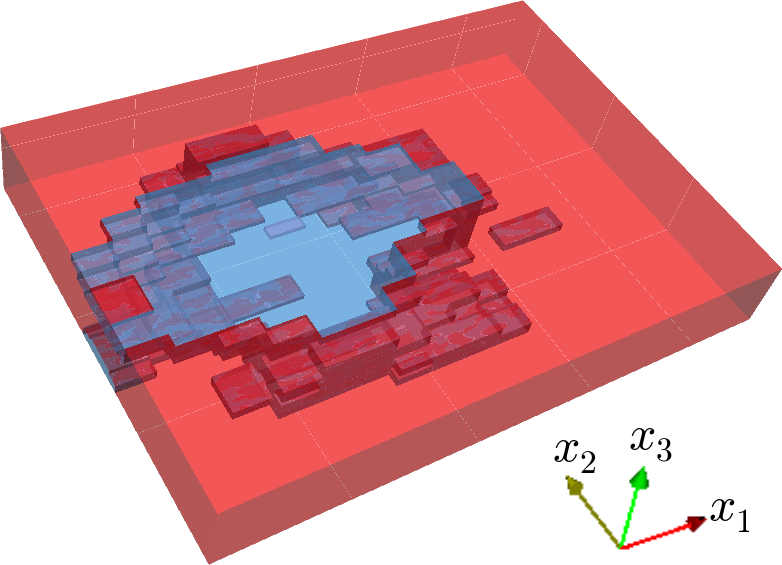
\includegraphics[width=0.31\textwidth]{series3D/run_diff_mesh/divvy4_whitebg_puff.png} 
}
\subfloat[MF$_5$ ($27.7\%$ HF)]{
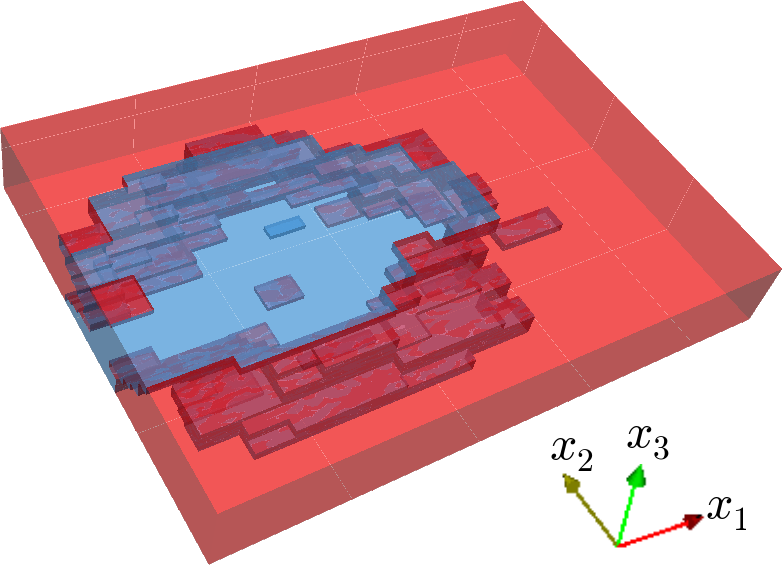
\includegraphics[width=0.31\textwidth]{series3D/run_diff_mesh/divvy5_whitebg_puff.png} 
}
\caption{Domain division for mixed-fidelity models: low-fidelity convection-diffusion model used in red portion, high-fidelity convection-diffusion-reaction model used in blue portion (intermediate colors due to transparency indicate a mix of the two models along the line of sight); $x_3$ direction scaled for clarity.}
\label{fig:divvy3D_diffmesh}
\end{figure} 
%
In this case, although the mixed-fidelity models have fewer degrees of freedom than the high-fidelity model, it is faster to solve the high-fidelity inverse problem than to adaptively seek a mixed-fidelity model with a small QoI error, starting from the low-fidelity model. This can be attributed to multiple factors: the high-fidelity problem is mildly nonlinear and has a close initial guess that is a solution to a linear system (when $k_r=0$), and the supplementary adjoint is solved on the high-fidelity mesh. Generally, one would expect solving the high-fidelity inverse problem to require more time relative to using the adaptive algorithm as the nonlinearity of the high-fidelity model increases. 

To illustrate the first offline-online application described in \cref{sec:onoff}, we generate ten sets of noisy observations to represent the actual data gained during the online phase; the noisy observations are generated by taking the observations used in the adaptive algorithm and adding Gaussian white noise with standard deviation of $\sigma=0.02$ (equivalent to, on average, $5\%$ of the observed values). We then solve the inverse problem using each of the mixed-fidelity models depicted in \cref{tab:ref3D_diffmesh,fig:divvy3D_diffmesh} as well as the high-fidelity model. The low-fidelity inverse problem is first solved and used as an initial guess for the higher-fidelity problems; we note that although there is a linear model that is more similar to the high-fidelity model than the low-fidelity model (i.e., convection-diffusion with anisotropic diffusivity and $k_r=0$ on the high-fidelity mesh) and thus would serve as a better initial guess, its existence is specific to our particular choice of models. The auxiliary and supplementary adjoint variables simply have a zero initial guess. 

\Cref{tab:ref3D_newdata_QoI_diffmesh} shows the average QoI values and error estimates and solution times for the (non)linear solves. \Cref{tab:ref3D_newdata_times_diffmesh} shows the times needed to solve the inverse problems and to solve for the additional variables needed to obtain an error estimate. For six of the ten datasets, the high-fidelity inverse problem does not converge given the low-fidelity solution as an initial guess; these are solved using the $k_r=0$ solution as an initial guess so that true QoI errors can be calculated. The average time high-fidelity inverse problem solution time shown in \cref{tab:ref3D_newdata_times_diffmesh} includes only those that converged with the low-fidelity initial guess.  
%
\begin{table}
\caption{Average QoI values and errors from solving inverse problem with mixed- and high-fidelity models and noisy data; relative errors are with respect to true high-fidelity QoI.}
\label{tab:ref3D_newdata_QoI_diffmesh}
\centering
\begin{tabular}{|c|c|c|c|c|c|}
\hline
\multirow{2}{*}{Case} & \multirow{2}{*}{$\%$HF} & \multirow{2}{*}{QoI} & Error & Error & $\%$ Relative  \\ 
& & & (Estimated) & (Actual) & Error (Actual) \\ \hline
LF   & 0    & 166774 & --    & -84326 & -102.3 \\
MF01 & 5.2  & 164597 & 4347  & -82149 & -99.65  \\
MF02 & 11.4 & 88867  & -5921 & -6418  & -7.79  \\
MF03 & 16.3 & 85237  & -2414 & -2789  & -3.38  \\
MF04 & 22.0 & 83411  & -724  & -963   & -1.17  \\
MF05 & 27.7 & 82664  & -18   & -216   & -0.26 \\
HF   & 100  & 82500  & --    & --     & --  \\ \hline
\end{tabular}
\end{table}

%
\begin{table}
\caption{Average times to solve inverse problem and obtain error estimate with mixed- and high-fidelity models and noisy datasets.}
\label{tab:ref3D_newdata_times_diffmesh}
\centering
\begin{tabular}{ccc|c|c|c}
\cline{4-5} 
 & & & \multicolumn{2}{|c|}{Error Estimation} & \\
\cline{1-6}
\multicolumn{1}{|c|}{\multirow{3}{*}{Case}} & \multicolumn{1}{|c|}{\multirow{3}{*}{DOFs}} & Inverse & Auxiliary & Supplementary & \multicolumn{1}{|c|}{Total} \\
\multicolumn{1}{|c|}{} & \multicolumn{1}{|c|}{} & Problem & Variables & Adjoint & \multicolumn{1}{|c|}{Solution}\\
\multicolumn{1}{|c|}{} & \multicolumn{1}{|c|}{} & Time (s) &  Time (s) & Time (s) & \multicolumn{1}{|c|}{Time (s)}\\
\cline{1-6}
\multicolumn{1}{|c|}{LF}    & \multicolumn{1}{|c|}{9537}   & 16   & --  & -- & \multicolumn{1}{|c|}{--} \\ \hline
\multicolumn{1}{|c|}{MF01}  & \multicolumn{1}{|c|}{13147}  & 185  & 107 & 235 & \multicolumn{1}{|c|}{526} \\ \hline
\multicolumn{1}{|c|}{MF02}  & \multicolumn{1}{|c|}{17895}  & 328  & 169 & 206 & \multicolumn{1}{|c|}{703} \\ \hline
\multicolumn{1}{|c|}{MF03}  & \multicolumn{1}{|c|}{21001}  & 435  & 202 & 185 & \multicolumn{1}{|c|}{821} \\ \hline
\multicolumn{1}{|c|}{MF04}  & \multicolumn{1}{|c|}{24528}  & 406  & 201 & 188 & \multicolumn{1}{|c|}{795} \\ \hline
\multicolumn{1}{|c|}{MF05}  & \multicolumn{1}{|c|}{27984}  & 498  & 263 & 198 & \multicolumn{1}{|c|}{959} \\ \hline
\multicolumn{1}{|c|}{HF}    & \multicolumn{1}{|c|}{70785}  & 1185 & --  & --  & \multicolumn{1}{|c|}{1185} \\ \hline
\end{tabular}
\end{table}
%
We see that the mixed-fidelity models, when applied to noisy datasets different from that with which they were generated, continue to perform well in achieving a small error in the QoI while limiting the use of the high-fidelity model to less than a third of the domain. Given the same initial guess, the mixed-fidelity inverse problems takes less time on average than the high-fidelity inverse problem to solve, and they converge consistently. 

In testing this online-offline setting with a larger range of datasets, we would like to note some additional observations. Suppose one has two datasets $d_1$ and $d_2$, the latter of which one wishes to perform inference. For a fixed proportion of domain refinement, a mixed-fidelity model that was adaptively generated $d_2$ gives a smaller QoI error than a mixed-fidelity model that was generated based on $d_1$. The performance gap tends to widen as the two datasets become more different. Suppose one generated $d_1$ using the high-fidelity model $d_2$ using a model which differed from the high-fidelity model in its domain, boundary conditions, and reaction coefficient; then a mixed-fidelity model adaptively formed based on $d_1$ might not give a low QoI error when used to infer from $d_2$. However, when the adaptivity algorithm is directly applied to this $d_2$, it is still able to find a mixed-fidelity model with a low QoI error. This behavior suggest that, if resources allow, it is best to perform the adaptivity online with the true observations. If one is confident that one's high-fidelity model is a good approximation of reality, then the online-offline approach can potentially give a faster yet accurate QoI estimate.

\section{Conclusion}\label{sect:conc}

We have presented an error estimator that can be used to adaptively create a mixed-fidelity model with which to solve a goal-oriented inverse problem, so as to minimize the error in the QoI calculated from the inferred parameters. We applied this method to pairs of low- and high-fidelity models of convection-diffusion-reaction phenomena and were able to obtain QoI estimates with a small relative error without having to solve the inverse problem with the high-fidelity model. In these cases, the localization of the error estimate also indicated regions of the domain that were important to the interaction of the observations and the QoI.

%------------------------------------------------------------%
\section{Future Work} 
%------------------------------------------------------------%

A direction for extension of this work is to the case of the statistical inverse problem. Thus far in this work, we have considered the deterministic inverse problem, as described in \Cref{sec:setup}; we seek to infer the parameter values that optimally fit the observations and the prior beliefs embedded in the regularization. However, we can rarely, if ever, be certain that the inferred values are correct, whether this be due to epistemic uncertainty from a lack of knowledge or aleatoric uncertainty from inherent variability in the physical system, or both \cite{Ober04}. One may attempt to capture the uncertainty in the inferred parameters by representing them as random variables with a probability distribution; inferring the distribution of the parameters given some observations is the statistical inverse problem. 

The statistical inverse problem is often solved in a Bayesian framework. Bayes' rule is used to combine a prior distribution, which captures prior beliefs about the parameters, and a likelihood distribution, which captures the likelihood of observations given an instance of the parameter values and a model of noise in the observations, to give a posterior distribution on the parameters. Since there is generally no analytical expression for this posterior distribution, it is usually characterized by samples from the distribution. Sampling methods like the widely-used Markov chain Monte Carlo (MCMC) method require many evaluations of the forward model, and since the number of samples needed grows exponentially with the dimension of the parameter space, this problem becomes intractable for large parameter spaces. In engineering contexts, it is still usually the case, however, that we are ultimately interested in a low-dimensional QoI, and it is the uncertainty in this low-dimensional quantity that we wish to capture; this low-dimensional distribution is referred to as the predictive posterior.

One way we could potentially apply this work to the statistical inverse problem is by reducing the parameter space that needs to be sampled. Such a direction is suggested by the results presented in \Cref{sec:diffvcdr3D}, where the mixed-fidelity model had significantly fewer degrees of freedom in its parameter field than the high-fidelity model, and thus a smaller parameter space. In the case of a linear model and observation operator with a Gaussian prior and additive Gaussian noise, there are parallels between the objective function of the deterministic inverse problem with Tikhonov regularization and the mode of the posterior distribution. In \cite{Martetal12}, a method is described for creating proposal distributions, drawing from these parallels; both the linear Gaussian and nonlinear cases are addressed. Similarly, these parallels could potentially be drawn upon to extend this work to the creation of an alternative statistical inverse problem that, by utilizing a mixed-fidelity model with fewer degrees of freedom in its parameter field, requires exploration of a small parameter space with minimal compromise in the predictive posterior.

Another potential approach would be to extend our method to the creation of mixed-fidelity models that are used as surrogates; these surrogate models can be evaluated in place of the high-fidelity model, thus decoupling the number of expensive forward evaluations of the high-fidelity model needed from the number of posterior parameter distribution samples that is desired \cite{Con14}. The samples obtained using such a surrogate might sacrifice accuracy in representing the posterior parameter distribution for accuracy in representing the predictive posterior distribution. 

%other directions for extensions that I can't seem to fit in:
%mixing models in time as well? (different mixes of models at different time steps?)
%superadj on intermediate mesh; preliminary results suggest that error estimates remain reasonable and generation of mixed-fidelity models can continue despite the additional approximations to the supplementary adjoint 

%\item \Cref{alg:refSeries} is also ammenable to an offline-online decomposition, analagous to that proposed in \cite{LiebWill13}. In the case where both the low-fidelity and high-fidelity inverse problems are linear in the data, and the QoI is linear in the state and parameters, one may first compute and store the supplementary adjoint $\Lambda_0$ for the low-fidelity model. As new data is received, one can compute the $\Psi_{LF}$ for this new data; evaluating \cref{eq:finErrExp} with the stored $\Lambda_0$ and the new $\Psi_{LF}$ gives an exact estimate of the error in the QoI, and thus effectively the high-fidelity QoI (NOT TRUE the primary and aux vars appear in the rhs...). When these linearities do not all hold, one cannot obtain an exact error estimate. The offline phase would consist of adaptively creating a mixed-fidelity model with an appropriate error tolerance given some expected observations $d^*$, and storing its suppementary adjoint $\Lambda_{MF}^*$. As new data is received, one can compute the $\Psi_{MF}$ for the mixed-fidelity model and the new data; evaluating \cref{eq:finErrExp} with the stored $\Lambda_{MF}^*$ and the new $\Psi_{MF}$ gives an estimate of the error in the QoI, and thus an effective estimate of the high-fidelity QoI. 


\section*{Acknowledgements}

This work was supported by the U.S. Department of Energy Office of Science, Office of Advanced Scientific
Computing Research, Applied Mathematics program under Award Number DE-FC02-13ER26129/DE-SC0009297 as part of the
DiaMonD Multifaceted Mathematics Integrated Capability Center.


\bibliographystyle{siamplain}
\bibliography{masterBib}
\end{document}
